% arara: pdflatex: {synctex: yes, action: nonstopmode}
% arara: pdflatex 
% arara: bibtex 
% arara: pdflatex
% arara: pdflatex
% arara: nomencl
% arara: pdflatex: {synctex: yes, action: nonstopmode}

%\documentclass[a4crop]{ntnuthesis} 
\documentclass{ntnuthesis}  
\usepackage{amsmath} %equations and spacings
\usepackage[utf8]{inputenc}
\usepackage{lipsum} % acces to random text
%graphics
\usepackage{graphicx}
%\usepackage[demo]{graphicx}
%caption styles
\usepackage[small,bf]{caption}
%\usepackage{caption}
\usepackage[labelformat=simple]{subcaption}
\renewcommand\thesubfigure{(\alph{subfigure})} % see subcaption doc
%<<byman 
\usepackage{colortbl}
\usepackage{xcolor}
\usepackage{color}
\usepackage{sidecap}
%byman>>

%<<byman
%% We want UK-english hyphenation patterns.byman
\usepackage[british]{babel}
%byman>>

%Remove Paragraph indenting
\setlength{\parindent}{0.0in} 
\setlength{\parskip}{0.1in}

%<<byman
%% Use scalable, PostScript Type 1 versions of the Computer Modern fonts.
\usepackage{type1cm}
%% Replace the standard Computer Modern Typewriter font LaTeX uses
%% for monospace text with the PostScript font Adobe Courier.
\usepackage{courier}
\usepackage[T1]{fontenc}
\usepackage{ae,aecompl}
\usepackage{times}
%% Redefine the font used for the section headings to
%% Helvetica-Narrow Bold.
\usepackage{sectsty}
\allsectionsfont{\usefont{OT1}{phv}{bc}{n}\selectfont}
% for colour shades in tables 
\usepackage{colortbl} 
 %to control the title formating and spaces around the titles
 \usepackage{pdfpages}
\usepackage[compact]{titlesec}
%%byman>>


%spaces under sections
\usepackage[compact]{titlesec}
\titlespacing{\section}{0pt}{*0}{*0}
\titlespacing{\subsection}{0pt}{*0}{*0}
\titlespacing{\subsubsection}{0pt}{*0}{*0}
%fonts
 %\usepackage[T1]{fontenc} %gives light font
 %\usepackage[light,math]{iwona}

%Abbreviations or Acronyms
%\usepackage[intoc]{nomencl}
\usepackage{nomencl}
\renewcommand{\nomname}{List of Abbreviations}
\makenomenclature

%Bibliography
%\usepackage{url}
\usepackage[]{natbib}%\usepackage[sectionbib]{natbib}
\usepackage{chapterbib}
%\bibpunct[:]{(}{)}{;}{a}{}{,} %citation structure
\bibpunct{(}{)}{,}{a}{}{;} 
%\bibpunct{[}{]}{,}{a}{}{;}
%\bibpunct{(}{)}{;}{a}{}{,} % to follow the A&A style
%\usepackage{chapterbib}
\usepackage{hyperref}
%\hypersetup{colorlinks=true,citecolor=blue}
\hypersetup{colorlinks=true,citecolor=blue,linkcolor=blue,urlcolor=blue}

%To change box color around the links and citations, you have these other options :
%\hypersetup{citebordercolor=Violet,filebordercolor=Red,linkbordercolor=Blue}

\newcommand{\cmt}[1]{}%inline comment
  
%tabularx
\usepackage{tabularx}
\usepackage{tabulary}
\usepackage{longtable} %table on several pages
\usepackage{booktabs}

%enumerate(control spacing)
\newenvironment{packed_enum}{
\begin{enumerate}
	\vspace*{-1}
  	\setlength{\itemsep}{1pt}
  	\setlength{\parskip}{0pt}
  	\setlength{\parsep}{0pt}
}{\end{enumerate}}

%<<byman
\usepackage{multirow}
\usepackage{dcolumn}
\newcolumntype{d}{D{.}{.}{-2}}
\newcommand{\tabincell}[1]{\begin{tabular}{c}#1\end{tabular}}
\newcommand{\tabincellt}[1]{\begin{tabular}{l}#1\end{tabular}}
\newcommand{\merge}[1]{\multicolumn{1}{c}{#1}}

\usepackage{array}
\newcommand{\PreserveBackslash}[1]{\let\temp=\\#1\let\\=\temp}
\newcolumntype{C}[1]{>{\PreserveBackslash\centering}p{#1}}
\newcolumntype{R}[1]{>{\PreserveBackslash\raggedleft}p{#1}}
\newcolumntype{L}[1]{>{\PreserveBackslash\raggedright}p{#1}}

% Used to create tables with rows/cols spanning over se
%% Use fancy chapter headers, with Jos Dingjan's modifications,
%% plus my own tweaks. This style is not part of teTeX,
%% so we are using a local (and renamed) copy.
%\usepackage[Lenny]{fncychapleo}
\usepackage{fncychap}

%% Nicely format and linebreak URLs in the bibliography (and elsewhere).
%%\usepackage{url}
%% Define a new 'leo' style for the package that will use a smaller font.
\makeatletter
\def\url@leostyle{%
  \@ifundefined{selectfont}{\def\UrlFont{\sf}}{\def\UrlFont{\small\ttfamily}}}
\makeatother
%% Now actually use the newly defined style.
\urlstyle{leo}
%byman>>

%graphics
\usepackage{epstopdf} %support for eps.
\DeclareGraphicsExtensions{.eps,.ps,.pdf,.png,.jpg}
\usepackage{float} % figure placing [H]

%landscape Option
\usepackage{lscape} %Left down
%usepackage{pdflscape} %Left up)

\usepackage[draft]{todonotes}   % notes showed (JJUNJU)
% Select what to do with command \comment:  
% \newcommand{\comment}[1]{}  %comment not showed
\newcommand{\comment}[1]
{\par {\bfseries \color{red} #1 \par}} %comment showed

%Section Numbering and TOC depth
\setcounter{secnumdepth}{2}
\setcounter{tocdepth}{3}

%chapter biblio
\usepackage{chapterbib}


\usepackage{tikz-timing}
\usepackage{todonotes}
\usepackage{cleveref}

%Drawing flow charts
\usepackage{tikz}
\usetikzlibrary{shapes,arrows,arrows.meta,quotes}
\tikzstyle{decision} = [diamond, draw, fill=blue!20, 
    text width=4.5em, text badly centered, node distance=3cm, inner sep=0pt]
\tikzstyle{process} = [rectangle, draw, fill=blue!20, 
    text width=5em, text centered, rounded corners, minimum height=4em]
\tikzstyle{line} = [draw, -latex']
\tikzstyle{output} = [trapezium,draw, trapezium left angle=70,trapezium right angle=-70,fill=pink, text width=3em, minimum height=2em,text centered]
\tikzstyle{data} = [trapezium,draw, trapezium left angle=70,trapezium right angle=-70,fill=white!20, text width=3em, minimum height=2em,text centered]
\tikzstyle{space} = [rectangle, fill=white,opacity=0,text width=5em, text centered, rounded corners, minimum height=4em]
\tikzstyle{results} = [ellipse,draw,fill=white, text width=4em, minimum height=3em,text centered]

%To generate list of symbols
\newcommand{\addsymbol}[3]{%
  \symboldisplay{#1}{#2}\\%
  \setelem{#3}{#1}
}
\newcommand{\symboldisplay}[2]{%
  $#1$ \parbox{5in}{\dotfill #2}%
  %$#1$ \parbox{5in}{ #2}%
}
%\def\setelem#1{\expandafter\def\csname myarray(#1)\endcsname}
\def\setelem#1{\expandafter\gdef\csname myarray(#1)\endcsname}
\def\dispsymbol#1{\csname myarray(#1)\endcsname} 

%Titles
\title{Analysis of design parameters in a musical dual resonant solid state tesla coil}
%\subtitle{Subtitle of the thesis here}
\author{Øystein Smith}

\def \thesisAuthor{Øystein Smith}

%\degreetype{PhD}
\faculty{Faculty of Information Technology and Electrical Engineering}
\department{Department of Electronic Systems}
\copyrightnotice{All rights reserved}
\isbnprinted{}
\isbnelectronic{}
\serialnumber{}
\setyear{2017}
\setmonth{June}

\begin{document}

\frontmatter
\maketitle

%<<byman
%% Configuration of the header strings for the frontmatter pages.
\fancyhead[RO]{{\footnotesize\rightmark}\hspace{1em}\thepage}
\setcounter{tocdepth}{2}
\fancyhead[LE]{\thepage\hspace{1em}\footnotesize{\leftmark}}
\fancyhead[RE,LO]{}
\fancyhead[RO]{{\footnotesize\rightmark}\hspace{1em}\thepage}
%byman>>

%TOC
\tableofcontents
%\addcontentsline{toc}{chapter}{Contents}
\cleardoublepage

\listoftables	
\addcontentsline{toc}{chapter}{List of Tables}
\cleardoublepage

\listoffigures	
\addcontentsline{toc}{chapter}{List of Figures}
\cleardoublepage

%Abbreviations
\newpage
%\thispagestyle{empty}
\printnomenclature
\cleardoublepage

%Symbols
\newpage
\chapter*{List of Symbols\hfill} 
\addcontentsline{toc}{chapter}{List of Symbols}
\begin{flushleft}
	%\addsymbol{Driver}{Electronics for supplying signal and power to a coil rig forming a tesla coil}{}
%\addsymbol{Coil rig}{Coil inductors and capacitors forming a resonant circuit in the arrangement of a resonant transformer}{}
%\addsymbol{Primary resonant circuit}{The Coil inductor and capacitor on the primary side of the resonant transformer in a coil rig}{}
%\addsymbol{Secondary resonant circuit}{The Coil inductor and capacitor on the secondary side of the resonant transformer in a coil rig}{}

\textbf{Driver:} Electronics for supplying signal and power to a coil rig forming a tesla coil.

\textbf{Coil rig:} Coil inductors and capacitors forming a resonant circuit in the arrangement of a resonant transformer.

\textbf{Primary resonant circuit:} The Coil inductor and capacitor on the primary side of the resonant transformer in a coil rig.

\textbf{Secondary resonant circuit:} The Coil inductor and capacitor on the secondary side of the resonant transformer in a coil rig.

\end{flushleft}

\mainmatter

\cleardoublepage
%\input{F01-copyright}
%\input{F02-dedication}
%\input{F03-abstract}
%\input{F04-preface}
%\input{F05-acknowledgements}
%
%Chapters
%Introduksjon
\chapter{Introduction}
\label{intro}
Universities, science centers and other institutions has the need for equipment that demonstrates physical phenomena in interesting and audience friendly ways. An example of this is a Double Resonant Solid State Tesla Coil (DRSSTC). This is a contraption that by the use of high voltage generates a sequence of electrical discharges. When these discharges happen in air a sound wave is generated. By modulating the frequencies of these discharges one can generate sound with different tones. A DRSSTC can in this way be made into a musical instrument.
There is no big commercial or academic community for tesla coils, but tesla coils are mostly designed and used as a hobby. There are a few people sharing their designs on the internet that most of the tesla coil designs are based on. Few or none of these substantiate design choices or assumptions with physics and math. This thesis will attempt to substantiate the design choices done in the driver for a musical dual resonant solid state tesla coil.

\Cref{fig:teslabano} shows a DRSSTC in use with an electric discharge from the top to a grounded copper object.

\begin{figure}[ht]
    \centering
    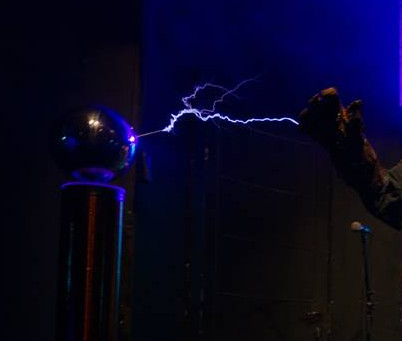
\includegraphics[width=0.6\textwidth]{img/teslabano.jpg}
    \caption{A tesla coil in use}
    Photo: Sindre Vaskinn Hunn
    \label{fig:teslabano}
\end{figure}

\section{Tesla Coil}
\label{tesla}
%http://www.tfcbooks.com/tesla/contents.htm
The Tesla Coil is a form of resonant transformer invented by Nikolai Tesla and used for experiments with artificial illumination \citep{5570149}. A resonant transformer consists of two inductively coupled coils, each loaded with a capacitance such that they get the same resonance frequencies. The resonant transformer has since gotten a lot of applications, among others; RFID \citep{b1960radio}, NFC \citep{5958681}, and Wireless charging \citep{5754800}. The resonant transformer in the form of the Tesla Coil has also become a popular entertainment device.
%Death ray
%Entertainment

\section{Earlier work}
%Who has done work on this before? steve4hv, pupman, scantesla, loneoceans.
Some of the people who have done work on DRSSTC in the hobbby community are; Steve Ward \Citep{stevehv}, Jimmy Hynes \Citep{chunkyboy86}, Terry Fritz \Citep{terrel}, Steve Conner \Citep{conner}, Dan McCauley \Citep{easternvoltage}, and the tesla coil mailing list \Citep{pupman}. Among these there are few disagreements on how a tesla coil should be designed, there are few variations on the resonant circuit, but slightly more variation on the low voltage controlling side. Some use a preset oscillator to drive the resonant circuit, while others use feedback from either the primary or secondary resonant circuits.

There has been developed an drsstc tesla coil driver by Steve Ward witch other people have designed variations on \Citep{ud27}.
Simulation software for the resonant circuitry of tesla coils called Scantesla have been written \Citep{scantesla}.
Guidelines for the design of the resonant circuits can be found at most of the above mentioned sites.

A modular back plane based tesla coil driver implementation have been designed and implemented by the author together with other members of Omega Verksted\footnote{Omega Verksted is a association of electronics and hobby interested students at the Norwegian University of Science and Technology (NTNU) founded in 1971.} \citep{prosjektoppgave} \citep{githubtesla}. This is based on earlier designs by members of Omega Verksted, the last major implementation at Omega Verksted was done in 2009 mostly by Dewald de Bruyn.

%Onetesla sells commercially

%Tables for coil aspect ratios.

\section{Overview}
This thesis will begin by discussing an implementation of a DRSSTC, substantiating the functionality of sub circuits with mathematics. Then discuss the mathematical description of the resonant transformer, varying component sizes, plotting and simulating the transfer functions. Then present some measurements done on a physical implemented DRSSTC.
%Beskrivelse av Tesla Coil / DRSSTC
%\section{Tesla Coil}
\label{tesla}
%http://www.tfcbooks.com/tesla/contents.htm
The Tesla Coil is a form of resonant transformer invented by Nikolai Tesla and used for experiments with artificial illumination \citep{5570149}. A resonant transformer consists of two inductively coupled coils, each loaded with a capacitance such that they get the same resonance frequencies. The resonant transformer has since gotten a lot of applications, among others; RFID, NFC, and Wireless charging. The resonant transformer in the form of the Tesla Coil has also become a popular entertainment device.
%Death ray
%Entertainment
%Tidligere arbeid
%\section{Earlier work}
%Who has done work on this before? steve4hv, pupman, scantesla, loneoceans.
There is no big commercial or academic community for tesla coils, but tesla coils are mostly designed and used as a hobby. There are a few people sharing their designs on the internet that most of the tesla coil designs are based on. Some of these are; Steve Ward \Citep{stevehv}, Jimmy Hynes \Citep{chunkyboy86}, Terry Fritz \Citep{terrel}, Steve Conner \Citep{conner}, Dan McCauley \Citep{easternvoltage}, and the tesla coil mailing list \Citep{pupman}.

Among these there is few disagreements on how a tesla coil should be designed, there are few variations on the resonant circuit, but slightly more variation on the low voltage controlling side. Some use a preset oscillator to drive the resonant circuit, while others use feedback from either the primary or secondary resonant circuits.

There has been developed an drsstc tesla coil driver by Steve Ward witch other people have designed variations on \Citep{ud27}.

Simulation software for the resonant circuitry of tesla coils called Scantesla have been written \Citep{scantesla}.

Guidelines for the design of the resonant circuits can be found at most of the above mentioned sites.

A modular back plane based tesla coil driver implementation have been designed and implemented by the author together with other members of Omega Verksted\footnote{Omega Verksted is a association of electronics and hobby interested students at the Norwegian University of Science and Technology (NTNU) founded in 1971.}. This is based on earlier designs by members of Omega Verksted, the last major implementation at Omega Verksted was done in 2009 mostly by Dewald de Bruyn.

Few or none of these substantiate design choices or assumptions with physics and math, this thesis will attempt to substantiate the design choices done in the driver for a musical dual resonant solid state tesla coil.

%Onetesla sells commercially

%Tables for coil aspect ratios.
%Teori? nei
%\chapter{Theory}
What do you need to know to read this report.
%\section{Audio}

%Klang
%Overtoner
%Subjektivt

%Beskrivelse av arkitektur (Blokkoppbygning)
\chapter{DRSSTC}
\label{DRSSTC}

\begin{figure}
    \centering
    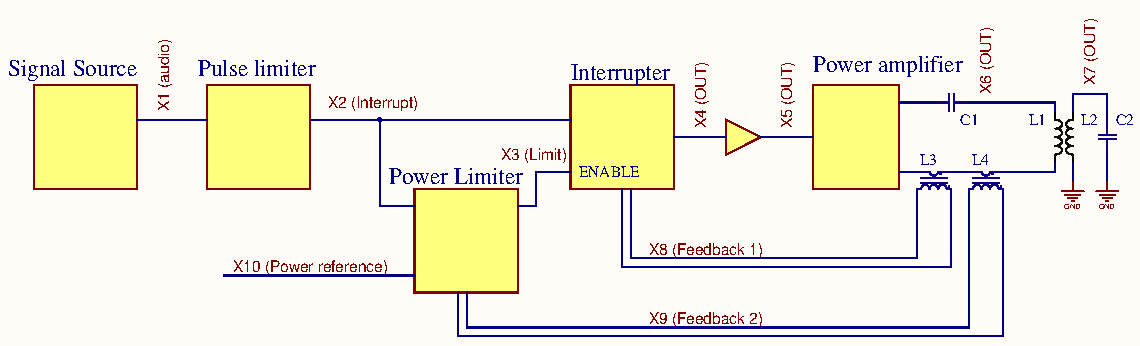
\includegraphics[width=\textwidth]{Skjema/FunksjonsBlokkskjema.pdf}
    \caption{Block diagram}
    \label{fig:func_block}
\end{figure}

\begin{figure}
    \centering
    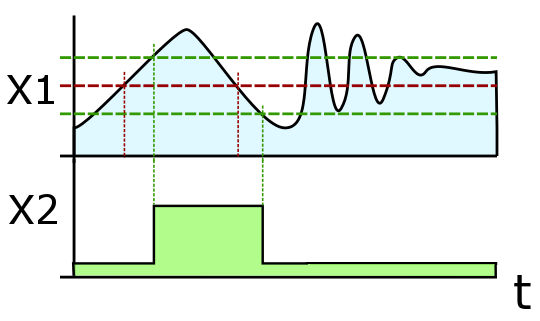
\includegraphics[width=\textwidth]{img/Smitt_hysteresis_graph_x1_x2.png}
    \caption{Tranformation of $X1$ to two level \citep{wikimedia}}       
    \label{fig:schmidt}
\end{figure}


In a DRSSTC dual resonant means that we have two resonant circuits inductively coupled, and tuned to the same resonance frequency. Solid state means that we drive these resonant circuits actively with transistors. The origins of the DRSSTC is not well documented but it is commonly accepted that it was conceived on "The tesla coil mailing list" \citep{pupman}.

The signal pathway consists of a signal source, pulse limiter, power limiter, interrupter, amplifier, and power amplifier see \cref{fig:func_block}.
The signal source provides the signal to be output on the coil, often the signal source is a musical recording.
The input signal should be monophonic, arpeggio\footnote{The sounding of the notes of a chord in rapid succession instead of simultaneously.} may be used. The input signal may be two level.

First the input signal $X1$ goes into the pulse shaper, which transforms the signal to two, level limits on-time of each pulse, and enforces a minimum time between pulses. In \cref{fig:schmidt} an example $X1$ is shown and a corresponding $X2$, here we see that the transformation to two level is done with a schmitd trigger, and that the pulses following immediately after the first pulse is suppressed. Then the signal $X2$ is connected to the interrupter which on a positive flank on $X2$ drives the resonant circuit at its resonant frequency until either the input pulse $X2$ goes low or the limit signal from the limiter $X3$ goes low.
The limiter measures the current flowing through $C_1$ and $L_1$. If the current exceeds a preset level $X10$ the limit signal $X3$ is set low until the next rising edge of the input signal $X2$. $X10$ is set by a multi turn potentiometer.

The resonant circuitry consists of $C_1$, $L_1$, $C_2$ and $L_2$, where $L_2$ is magnetically coupled with $L_1$ with a coupling coefficent of approximately $k=0.2$. $C_1$ is a bank of capacitors with high voltage and current rating and low equivalent series resistance (ESR). $L_1$ is an inductor with high cross section area and few turns (in the magnitude of 5 turns). $L_2$ is an inductor with low cross section area and a high number of turns (in the magnitude of 4000 turns). $C_2$ consists of a sphere or toroid for one plate, and the grounded (safety ground) surroundings. Ground is connected through the safety ground in the electrical socket used to power the DRSSTC. $L_3$ and $L_4$ are current sensing transformers used for feedback.

%Figure \cref{fig:scope} shows a measurement of these signals. Channel 2 (Green) shows the feedback signal $X8$ after it is fed through a protection network limiting the voltage (See the schematic for TK514 in appendix B). Channel 4 (Red) shows an internal signal $Y1 = X2$ \&\& $\overline{X3}$ in the interrupter. As long as this signal is high the output signal $X4$ will swing at the resonant frequency. Note that we would expect $X8$ to be zero as long as channel 4 is low, but there is some delay before the resonant circuit stops swinging after the supply of energy stops. Also note the interference on $X3$ and $Y1$ from the output signal $X6$.

%\begin{figure}
%    \centering
%    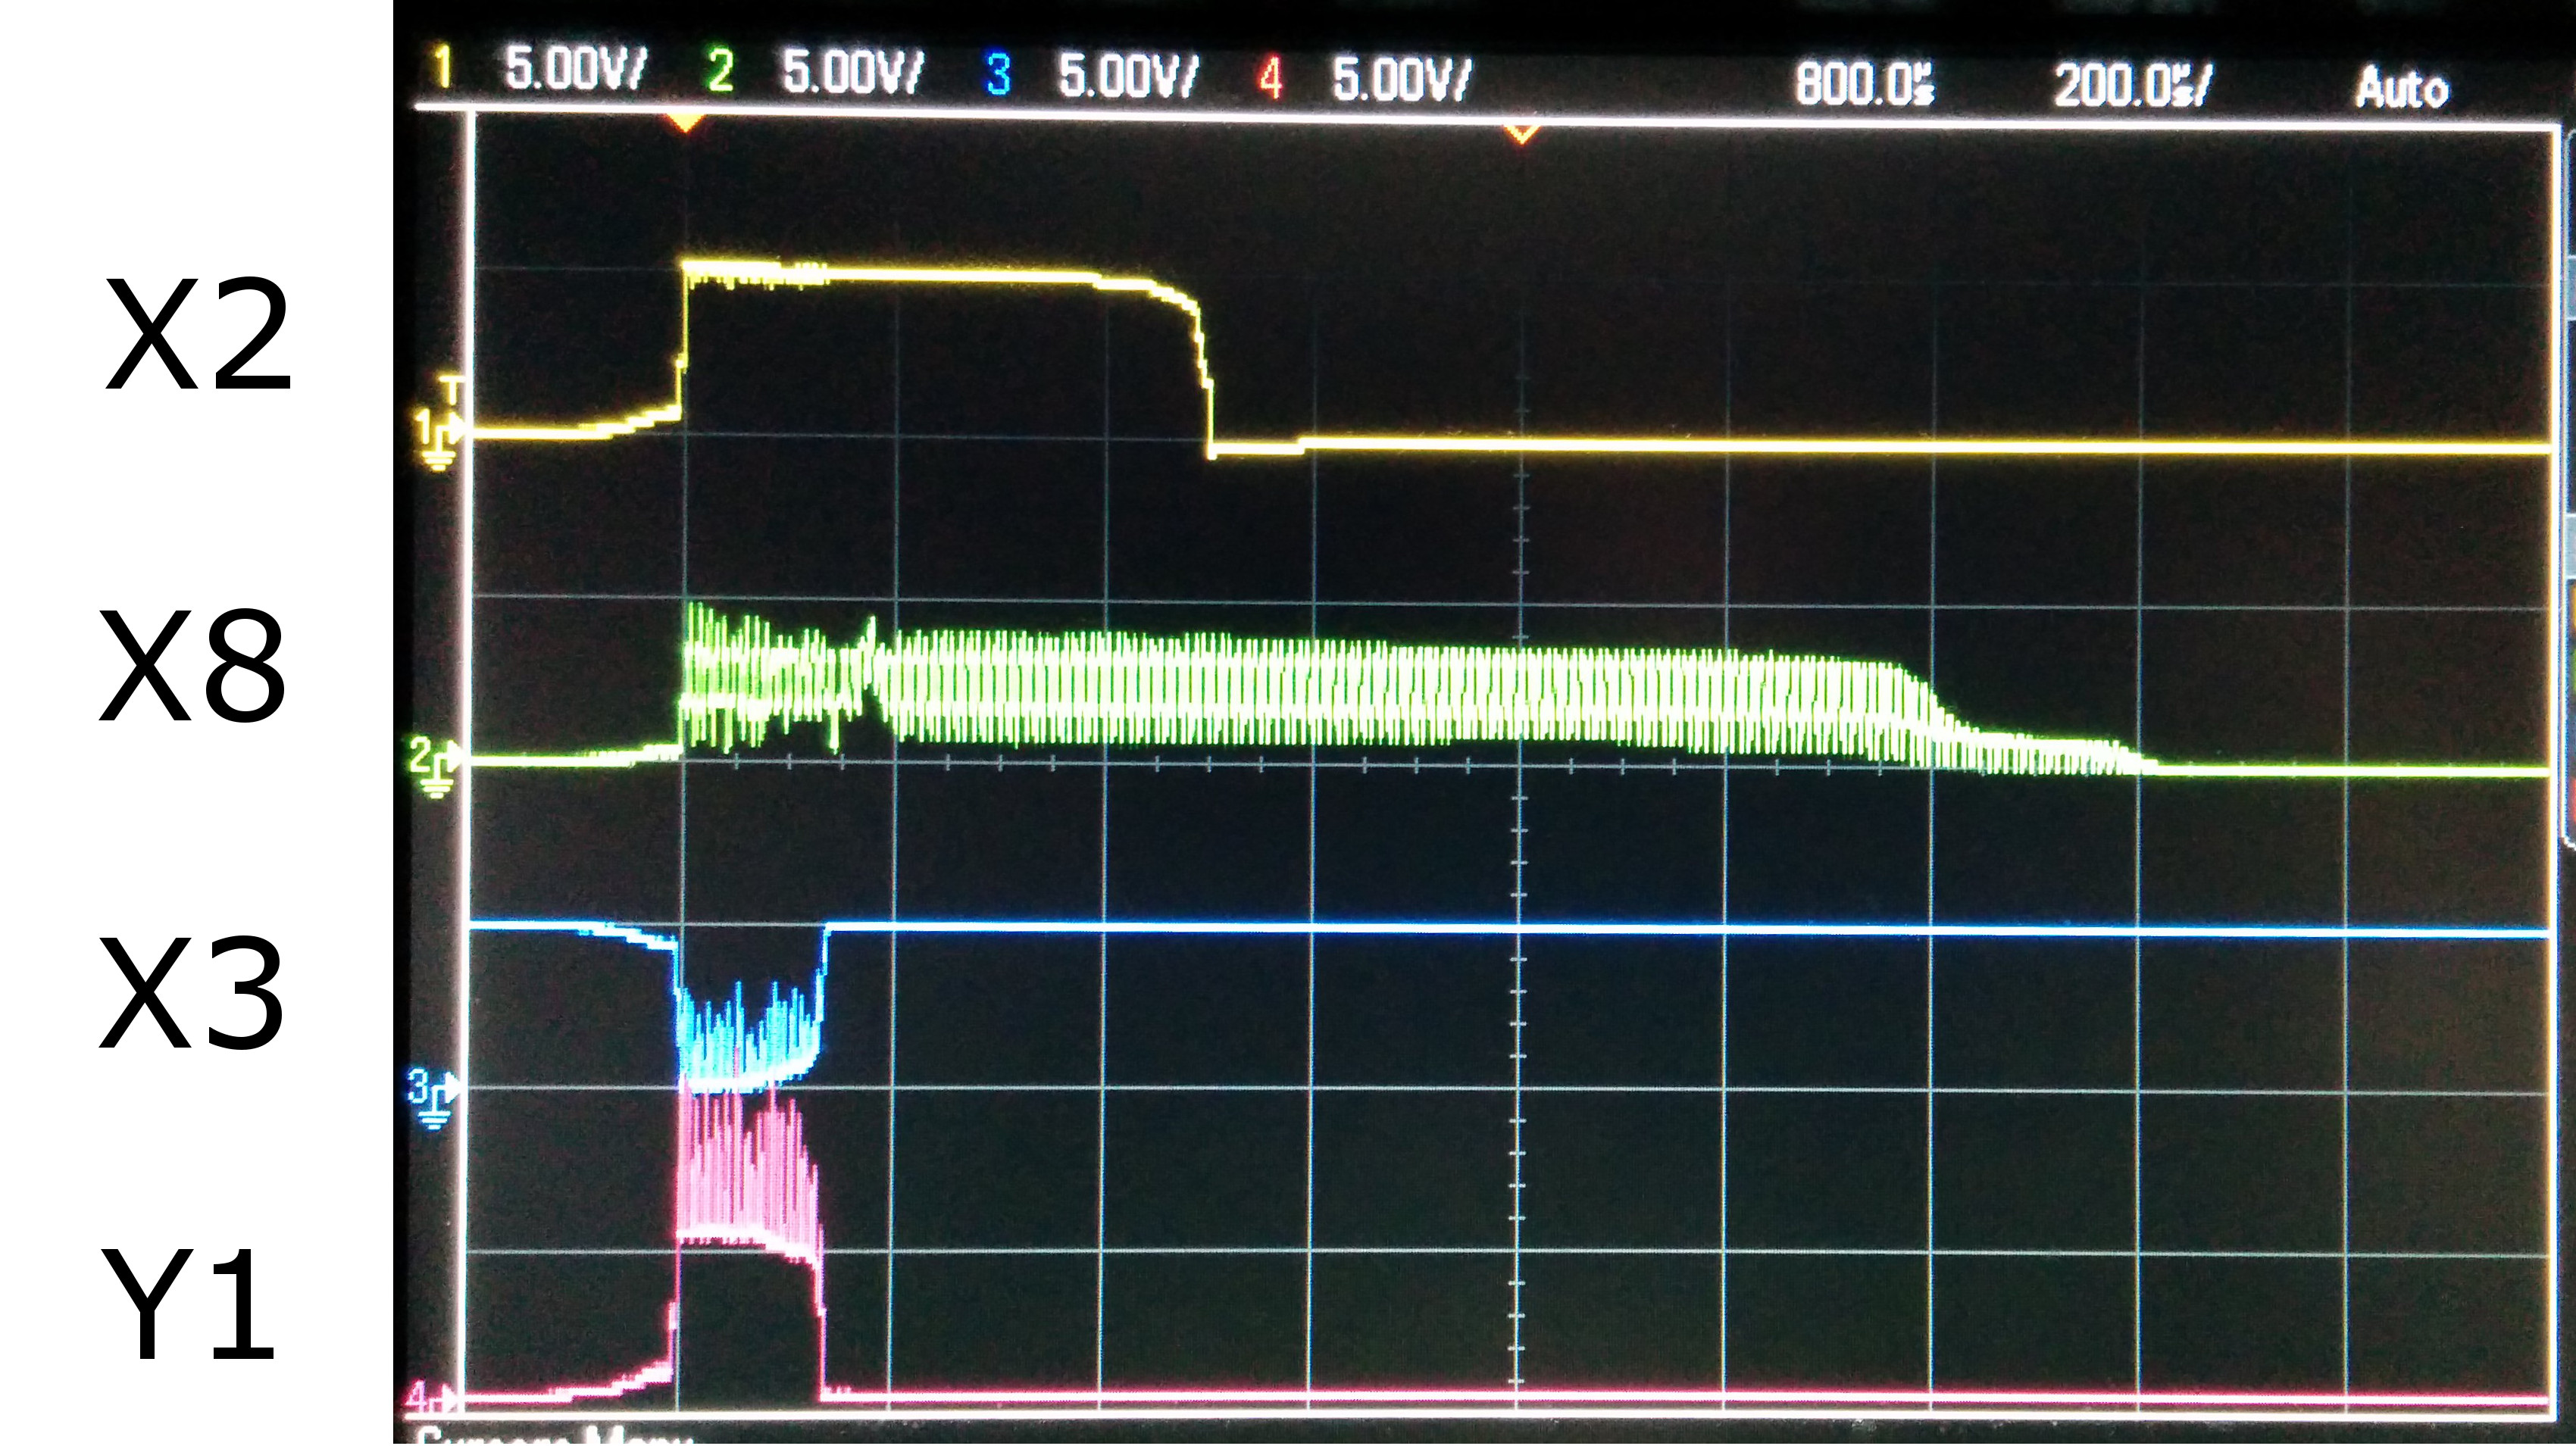
\includegraphics[width=\textwidth]{img/DRSSTC_scope.jpg}
%    \caption{Measurements of signals.}
%    \label{fig:scope}
%    Channel 1 (Yellow): $X2$, 2 (Green): $X8$, 3 (Blue) $X3$, 4 (Red): $X2$ \&\& $\overline{X3}$. Voltage axis: 5V/div. Time axis: $200\mu$s/div.
%\end{figure}

%Inngående beskrivelse av kretsene (inkludert designvalg)
%\begin{figure}[h!]
%    \centering
%    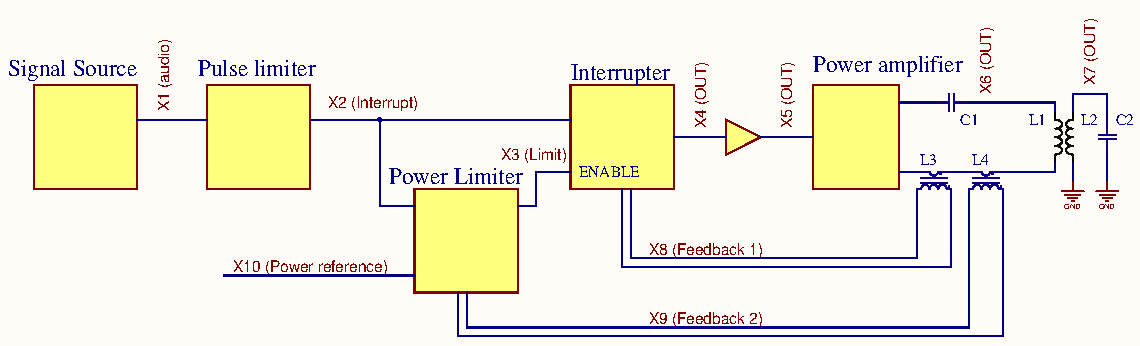
\includegraphics[width=\textwidth]{Skjema/FunksjonsBlokkskjema.pdf}
%    \caption{Block diagram}
%    \label{fig:block}
%\end{figure}

\section{Pulse shaper}
\label{sec:pulseshaper}
The purpose of the pulse shaper is to take the input signal $X1$ and transform it to be suitable for a DRSSTC, in addition to not letting harmful signals through. The pulse shaper in this implementation is built separate from the driver. The first step in the pulse shaper is to transform the input signal $X1$ to two level as shown in \cref{fig:x2detail}.

\begin{figure}[H]
\centering
    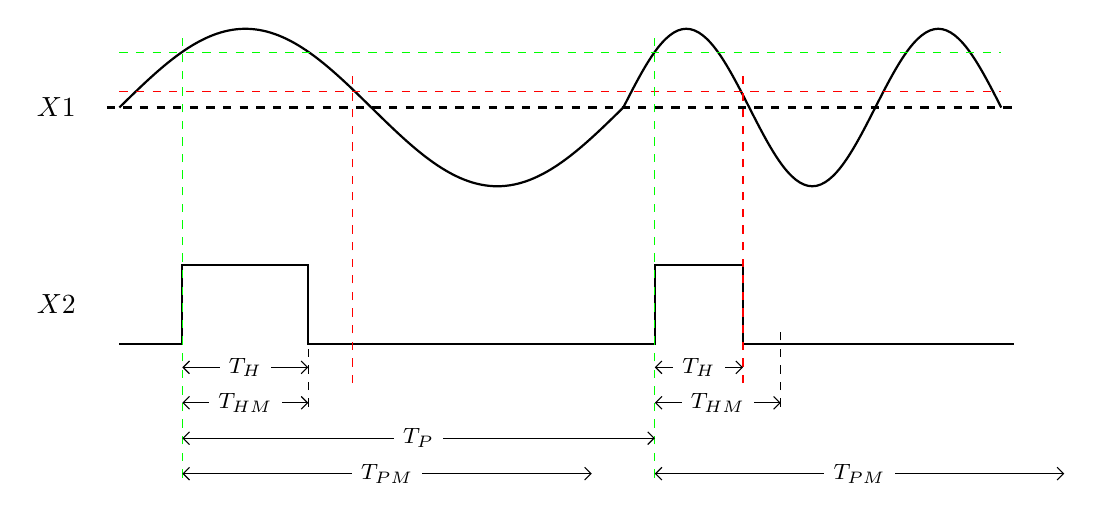
\begin{tikzpicture}[x=16mm,
        every edge/.style = {draw, Straight Barb-Straight Barb},
        every edge quotes/.style = {fill=white,font=\footnotesize}
        ]
    \draw[thick]
    (0.5,3) sin (1.5,4) cos (2.5,3) sin (3.5,2) cos (4.5,3) sin (5,4) cos (5.5,3) sin (6,2) cos (6.5,3) sin (7,4) cos (7.5,3);
    \draw[thick,dashed]  (0.4,3) -- (7.6,3);
    \draw[dashed,green]  (0.5,3.7) -- (7.5,3.7);
    \draw[dashed,red]  (0.5,3.2) -- (7.5,3.2);

    \draw (0,3) node {$X1$}; %label

    \draw[thick] (0.5,0) -- (1,0) -- (1,1) -- (2,1) -- (2,0) -- (4.75,0) -- (4.75,1) -- (5.45,1) -- (5.45,0) -- (7.6,0);
    \draw (0,0.5) node {$X2$}; %label

    \draw[dashed,green] (1.00,-1.7) -- ++ (0,5.6);
    \draw[dashed,red]   (2.35,-0.5) -- ++ (0,4);
    \draw[dashed,green] (4.75,-1.7) -- ++ (0,5.6);
    \draw[dashed,red]   (5.45,-0.5) -- ++ (0,4);
    
    \draw[dashed] (2.00,-0.8) -- ++ (0,1);
    \draw[dashed] (5.75,-0.8) -- ++ (0,1);

    \draw   (1.00,-0.30) edge ["$T_H$"]      (2.00,-0.30)
            (1.00,-0.75) edge ["$T_{HM}$"]   (2.00,-0.75)
            (4.75,-0.30) edge ["$T_H$"]      (5.45,-0.30)
            (4.75,-0.75) edge ["$T_{HM}$"]   (5.75,-0.75)
            (1.00,-1.20) edge ["$T_P$"]      (4.75,-1.20)
            (1.00,-1.65) edge ["$T_{PM}$"]   (4.25,-1.65)
            (4.75,-1.65) edge ["$T_{PM}$"]   (8.00,-1.65);
    \end{tikzpicture}
    \caption{Detail view of signal $X2$}
    \label{fig:x2detail}
\end{figure}{}

Here we see that the transformation to two level is done with a schmidt trigger, we also see that the pulse following immediately after the second pulse is suppressed wich will be explained below.

Then the triggering signal $X2$ is two level and contains two pieces of information from $X1$, the frequency $f_{X2}$ (tone) and the volume (intensity).

Where the frequency $f_{X2}=\frac{1}{T_P}$ is given by the time $T_P$ between the positive flanks of the signal. This is the base harmonic of the acoustic tone heard at the output of the system. The volume is given by the duty cycle of the pulses $D = \frac{T_H}{T_P}$. \Cref{fig:tones} shows different tones (varying $T_P$),

\begin{figure}[H]
    \centering
    \begin{tikztimingtable}
        $X2$ & 2L 1H 7L 1H 7L 1H 7L 1H 7L\\
        $X2$ & 2L 1H 5L 1H 5L 1H 5L 1H 5L 1H 5L 1H 1L\\
    \end{tikztimingtable}
    \caption{Different tones}
    \label{fig:tones}
\end{figure}{}

and \cref{fig:volumes} shows different volumes (varying $T_H$).

\begin{figure}[H]
    \centering
    \begin{tikztimingtable}
        $X2$ & 2L 1H 7L 1H 7L 1H 7L 1H 7L\\
        $X2$ & 2L 3H 5L 3H 5L 3H 5L 3H 5L\\
    \end{tikztimingtable}
    \caption{Different volumes}
    \label{fig:volumes}
\end{figure}{}

We also need to prevent harmful signals, meaning signals that may lead to destructive failure at the output. This is done by limiting the max duty cycle of the pulses as well as limiting the frequencies allowed. The duty cycle of the pulses is limited by choosing a maximum time $T_{HM}$ the pulse is allowed to be high, this time is independent of the frequency. This means the preset max duty cycle is dependent on the frequency of the pulse.
Limiting the frequencies allowed is done by choosing a minimum time $T_{PM}$ after a pulse goes high until $X2$ is allowed to go high again.

How this can be implemented is not discussed any further in this thesis. But this thesis should give the basis for choosing maximum and minimum values for $T_H$ and $T_P$.

\newpage
\section{Interrupter}
\label{sec:interrupter}

The interrupter generates the signal which drives the resonant circuit (coil rig) at its resonant frequency $f_0$. As long as the input signal $X2$ is high the output produces a square wave with fundamental frequency $f_0$. It does this by means of a positive feedback loop. The feedback signal $X8$ is retrieved with a sensing transformer around the output wire from the power amplifier (\cref{sec:pa}), before being clamped, rectified, and schmidt triggered. This results in a cleaned up normalized representation of $X8$, lets call this signal $X8'$. The flanks of $X8'$ represents when the output current passes zero (this is when we want to switch the polarity of the output $X5$). $X8'$ is fed to the output via gates controlled by a latch. $X5\_B$ is inverted in relation to $X5\_A$ (for push-pull operation). This circuit is shown in \cref{fig:interrupter}, U1A is the latch witch is central to the operation of the interrupter. It has Four inputs SD, CP, D, and RD, wich are 'Set Data' (active low), 'Clock Pulse', 'Data', and 'Reset Data' (active low) respectively. And two outputs; Q wich is the normal output, and Q inverted wich is the inverted of Q at all times, Q inverted is unused in this circuit.

\begin{figure}[H]
    \centering
    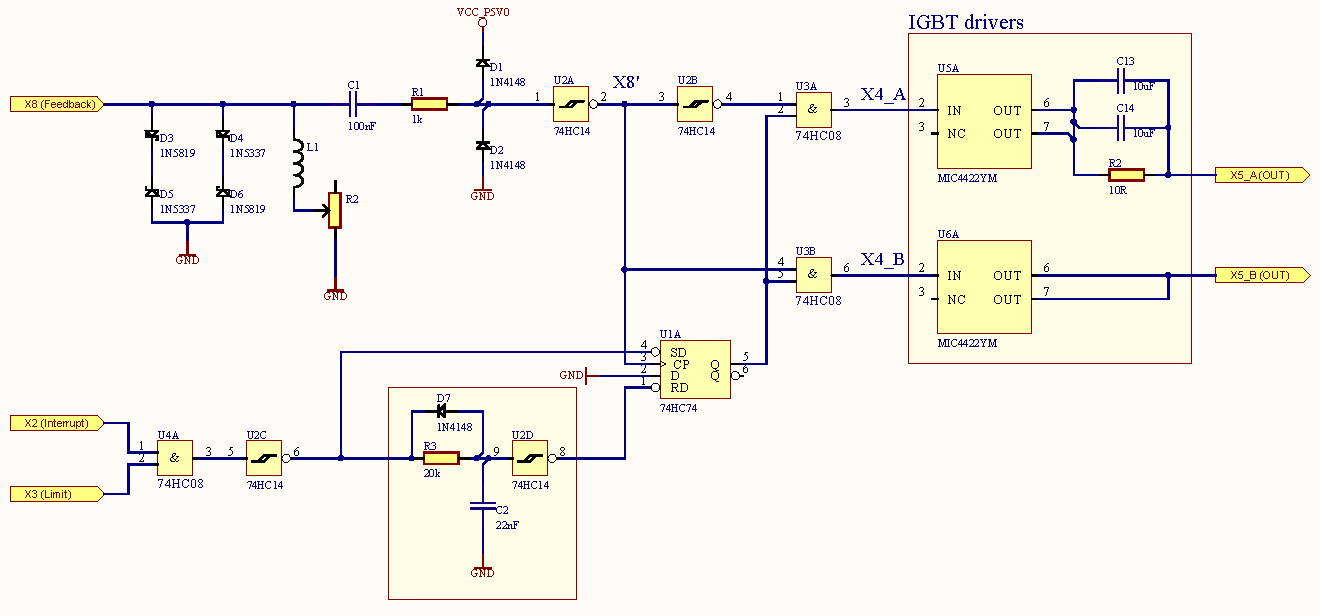
\includegraphics[width=0.9\textheight,angle=-90]{Skjema/TK514_Interrupter.pdf}
    \caption{Interrupter (TK514)}
    \label{fig:interrupter}
\end{figure}

\newpage

Initially no current is flowing in the resonant circuit therefore no voltage is present on $X8$, but because of C1 the the input of U2A is undefined. Let us look at the case of the output of U2A being high and the input $X2$ being low. Then the initial values of the signals are as shown in \cref{fig:int_timing}, SD is high (inactive) CP is high, D is low, RD is low (active), Q is low, $X4\_A$ and $X4\_B$ is low.

\begin{figure}[H]
    \centering
    \begin{tikztimingtable}
        $X2$      & 2L 19H 0.5H 10.5L\\
        $X8'$     & 2H 1H 19.5{1C} N(A1) 4{1C} 6H\\
        SD      & 2H 19L 0.5L 10.5H\\
        CP      & 2H 1H 24{1C} 5H\\
        D       & 32L\\
        RD      & 2L 28H 2L\\
        Q       & 2L 1H 19H N(B1) 10L\\
        $X4\_A$   & 2L 1L 19{1C} 10L\\
        $X4\_B$   & 2L 1H 19{1C} 10L\\
        \extracode
        \tablerules
        \begin{pgfonlayer}{background}
            \draw [help lines] (A1) -- (B1);
        \end{pgfonlayer}
    \end{tikztimingtable}
    \caption{Timing diagram for interrupter}
    \label{fig:int_timing}
\end{figure}{}

When $X2$ goes high the Set Data (SD) input of the latch U1A goes low and is activated, Reset Data RD goes high (inactive), and thus the output Q goes high. This enables the and gates U3A and U3B and allows X8' to pass through, $X4\_B$ goes high and $X4\_A$ remains low, this causes a step response in the resonant circuit. The feedback transformer is oriented such that this current direction gives a negative voltage on $X8$ and thus still low signal on the input of U2A. When the current direction changes the signal on the input of U2A goes from low to high and $X4\_A$ goes high and $X4\_B$ goes low. This reverses the voltage on the resonant circuit in phase with the step response and triggers an additional step response in phase with the already ongoing one. This cycle continues until $X2$ goes low. When $X2$ goes low SD goes low (inactive), but Q is still high until the next negative flank on $X8$ (inverted through U2A). When D (wich is strapped low) is clocked through the latch, Q goes low and both $X4\_A$ and $X4\_B$ goes low. And no further energy is supplied to the resonant circuit and the step response completes.
In the case of the initial value of the output of U2A being low $X4\_A$ would go high first instead of $X4\_B$ and $X8$ would go high right away. Prompting $X4\_A$ and $X4\_B$ to invert immediately and switch the output while the current is not zero. Then the rest of the events happen as explained above. This immediate inverting of $X4$ may be unfortunate and a pull down resistor should be added at the input of U2A. The resulting signal on the output $X7$ is then Pulse Density Modulated (PDM).

\subsubsection{Phase Lead}
\label{sec:phaselead}
The function of $L_1$ and $R_2$ is to introduce a phase lead on the voltage of $X8$ in relation of the current on $X8$. The purpose of this is to compensate for propagation delays in the circuit and for switching delays in the transistors in the power amplifier (\cref{sec:pa}). As the circuit is inductive, the voltage will lead the current. By adjusting the value of $R_2$ the relation between the inductance and resistance is changed and thus the phase angle is changed. Thus the time between when the voltage crosses zero and the current crosses zero can be adjusted. This time should theoretically be equal to the time it takes the feedback signal $X8$ to propagate through the logic and for the transistors (IGBTs) in the power amplifier to turn on or off. So that we will switch when the current in the resonant circuit is zero (Zero current switching). This is to reduce energy lost from the resonant circuit and to minimize power burned in the transistors (when switching). From the datasheets we have the propagation delays $t_{pd}$ for the different devices in the propagation path shown in \cref{tab:tpd}. The there are two propagation paths one path contains one schmidt trigger (74HC14) more than the other, also the propagation delay in the mosfet drivers (MIC4422YM) differs for rising and falling outputs. The average propagation delay $\overline{t_{pd}}$ from $X8$ on the input of U2A to $X5$ on the output of the mosfet drivers is then given by \cref{eq:tpd} and results in $\overline{t_{pd}} =$ 58 ns typical and 137,5 ns maximum.

\begin{table}[H]
    \centering
    \begin{tabular}{c|c|c|c}
                &   Device              & $t_{pd}$ Typ (ns)   & $t_{pd}$ Max (ns) \\
        $t_{inv}$ &   74HC14              & 12            & 25\\
        $t_{and}$ &   74HC08              & 10            & 20\\
        $t_{driv R}$& MIC4422YM Rising    & 20            & 80\\
        $t_{driv F}$& MIC4422YM Falling   & 40            & 80
    \end{tabular}
    \caption{Propagation delays for devices}
    \label{tab:tpd}
\end{table}

\begin{table}[H]
    \centering
    \begin{tabular}{c|c|c}
                            & $T_J = 25 ^{\circ}C$ & $T_J = 150 ^{\circ}C$ \\
        Turn-On Delay Time (ns)  & 46                & 31    \\
        Turn-Off Delay Time (ns) & 120               & 210
    \end{tabular}
    \caption{Turn on and off delays in the IGBT IRG4PC50WPbF}
    \label{tab:tigbt}
\end{table}

\begin{equation} \label{eq:tpd}
    \overline{t_{pd}} = t_{inv} + \frac{t_{inv}}{2} + t_{and} + \frac{t_{driv R}+t_{driv F}}{2}
\end{equation}

In addition the delays from hysteresis in U2A $t_h$ and switching delays in the transistors in the power amplifier $t_{sw}$ should be added to the desired phase lead $t_{d}$. Resulting in the desired phase lead $t_{d}$ being given by \cref{eq:td}.

\begin{equation} \label{eq:td}
    t_d = t_{h} + \overline{t_{pd}} + t_{sw}
\end{equation}

The feedback signal $X8$ should have sufficiently high voltage so that delays from hysteresis $t_h$ in U2A is neglible. Delays in the IGBT is read from the datasheet and presented in \cref{tab:tigbt}. If we add the delay at 25 $^{\circ}C$ to the nominal $t_d$ and the delay at 150$^{\circ}C$ to the maximum $t_d$, we get a $t_d$ of 141 ns nominal and 258 ns maximum.

Since there are no other resistances in the circuit than R2, as R1 is in series with both a capacitor and the input of the logic gate U2A and can be considered close to infinite in relation to R2, the phase angle is given by \cref{eq:theta}.

\begin{equation} \label{eq:theta}
    \theta = {\tan}^{-1}\frac{X_{L_1}}{R_2} = {\tan}^{-1}\frac{\omega L_1}{R_2} = {\tan}^{-1}\frac{2 \pi f_0 L_1}{R_2}
\end{equation}

And thus the desired phase lead is given by \cref{eq:tdl}, and the relation between $L_1$ and $R_2$ is given by \cref{eq:lr}.

\begin{equation} \label{eq:tdl}
    t_{d} = \frac{\theta}{\omega} = \frac{\theta}{2 \pi f_0}
\end{equation}

\begin{equation} \label{eq:lr}
    \frac{L_1}{R_2} = \frac{\tan(\theta)}{\omega} = \frac{\tan(\omega t_{d})}{\omega} = \frac{\tan(2 \pi f_0 t_{d})}{2 \pi f_0}
\end{equation}

Given $f_0$ = 110kHz and desired $t_d$ = 141 ns nominal and 258 ns maximum we get $\frac{L}{R} = 1,4 \cdot 10^{-7}$ s nominal and $\frac{L}{R} = 2,6 \cdot 10^{-7}$ s maximum. The total magnitude $|Z_L|$ of the impedance $Z_{L}$ of $L_1$ and $R_2$ should give a sufficiently high voltage $U_{X8}$ so that the delay due to hysteresis in U2A is negligible, but not too high voltage for the zener diodes D3-D6 to handle. The equation for $|Z_L|$ is shown in \cref{eq:zl}.

\begin{equation} \label{eq:zl}
    |Z_{L}| = \sqrt{{R_2}^2 + (2 \pi f_0 L_1)^2}
\end{equation}

The relation between the peak voltage $|U_{X8}|$ over $R_2$ and $L_1$ is shown in \cref{eq:ux8} assuming $X8$ is sinusiodal.

\begin{equation} \label{eq:ux8}
    |U_{X8}| = |Z_L| |I_{X6}| \frac{n1}{n2}
\end{equation}


\subsubsection{Reset network}
\label{sec:reset_net}
The function of the network connected to the reset (RD) of the latch (U1A) is to reset the latch after a delay in the case that a zero crossing is not detected on $X8$ after $X2$ goes low. Note the inverting schmidth triggers U2C and U2D on both sides of the network. When $X2$ goes high the input of U2D goes low immediately due to the capacitor $C_2$ being discharged through $D_7$, but when $X2$ goes low the capacitor $C_2$ will be charged through $R_3$ and there will be a delay before the latch is reset. The time constant of $R_3$ $C_2$ is $\tau = 440 \cdot 10^{-6} s$, the positive going threshold voltage of the inverting schmitt trigger (74HC14) is $T^+ = 2,5V$ Wich is half of the supply voltage VCC\_P5V0. We know that a capacitor is charged to $0,5 \cdot$ VCC (where VCC is the applied voltage) after $0,7 \tau$, thus the filter $R_3$ $C_2$ together with U2D introduces a delay of $0,7 \tau = 308\mu s$, or if we have a resonance frequency $f_0$ of 110 kHz a delay of about 3,4 periods $T = \frac{1}{f_0}$. If the synchronous shutdown does not work properly this filter should prevent or reduce noise from the interrupter not shutting down properly between each pulse on the input signal X2. This can also reduce the spark length if the spark is prevented from unintentionally continue longer than intended.

\subsubsection{Input clamping and protection}
$D_3$-$D_6$ are protection diodes which clamp the feedback signal to safe voltages. The network $L_1$ and $R_2$ introduces a tunable phase lead on the voltage. $C_1$ and $R_1$ is a filter to remove noise. $D_1$ and $D_2$ clamps the voltage to 0-5V.

\subsubsection{IGBT Drivers}
U5A and U6A are transistor drivers which amplify $X4$ and step up the voltage from 5V to 18V

%%%%%%% Stikkord
%The output of T1 is loaded with a pair of zener diodes with ultrafast diodes to block the slow recovery of the zeners (they are not allowed to be forward biased).  Since the transformer ratio is ~1:1000, by normal transformer action, the current should be 1/1000th of the primary current, and the voltage should be 1000X greater.

%The square wave is also passed through a capacitor to ensure only AC content is passed

%To further protect the logic gate of U1, we have a pair of fast logic diodes to clamp any voltage excursions to the supply rails.

%There are some tricks used to make the JK flip flop (U2) to operate properly in the circuit.  As shown when the interrupter goes HI, CLR\ is LOW.  This puts Q\ in a HI state.  Now, we see that there is a inverter (part of U1) that feeds from the interrupter signal, with its output feeding into an RC circuit and then another inverter.  What this does is delay the HI input to the PRE on the flip flop.  Note that before the PRE is HI, the output from the flip flop is whatever present on CLR\.  If we did not delay the input to PRE, then our interrupter pulse would never be passed along to the gate driver ENABLE (pin 3 on the UCC3732X).  Also note that the flip flop only does its synchronized shut down when PRE is high.  So this leads to choosing what value we want to use for the RC (R9 and C14).  I typically size it so that t=RC=1.5P, where P is the period (in seconds) for 1 RF cycle at the intended operating frequency.  Example, the DRSSTC-1 operates near 60khz, so 1 cycle is 16.67uS, so I would want an RC of about 25uS (whereas I use 22uS).  The important thing is that PRE does not go LOW before the flip flop does its synchronization.  You must allow for at least 1 full cycle of operation after the interrupter has gone LOW for the flip flop to act.  To be on the safe side, you could size the RC to be 3*P.

\newpage
\section{Power Limiter}
\label{sec:limiter}

The limiter prevents overcurrent in the coil rig by disabling the interrupter when the peak current rises above a preset level. The limiter is shown in \cref{fig:limiter}

\begin{figure}[H]
    \centering
    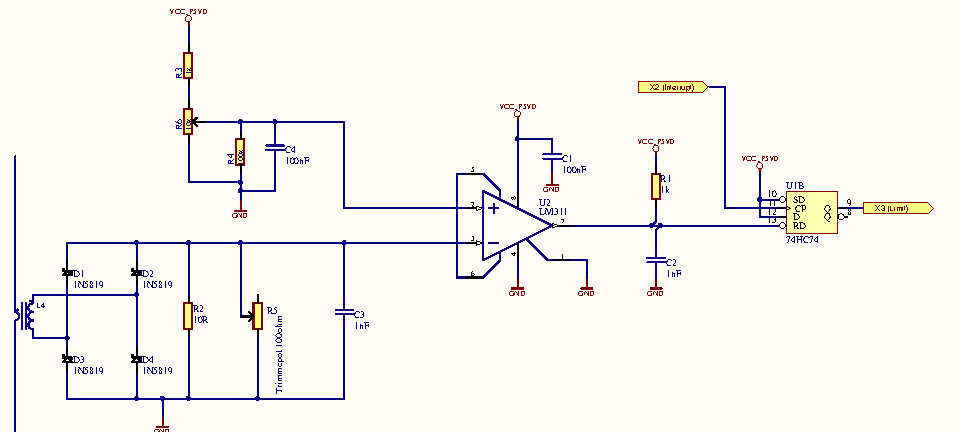
\includegraphics[width=\textwidth]{Skjema/TK513_Limiter.pdf}
    \caption{Limiter}
    \label{fig:limiter}
\end{figure}

The feedback signal is retrieved from the primary resonant circuit via the feedback transformer L4. The diodes D1-D4 is a full bridge rectifier, schottky diodes are used for low propagation delay. The rectifier is loaded with R2 and C3, R2 and C3 also functions as a noise filter with a cut off frequency $f_c$ given by \cref{eq:fc}.

\begin{equation} \label{eq:fc}
    f_c = \frac{1}{2 \pi R_2 C_3}
\end{equation}

The cut off frequency $f_c$ decides how much noise is allowed through to the comparator and thus how often the spark is shut down early unintentionally due to noise. The spark being shut down unintentionally generates noise on the acoustic signal.

The rectified signal is fed into a comparator, the other input of the comparator is connected to a variable voltage controlled by a potentiometer. R3 is to set the highest level the variable voltage can be set to. R4 is to pull the input of the comparator low in the case that the potentiometer is disconnected.

The relation between the (peak) current in the primary resonance circuit and the (peak) voltage on the input of the comparator is given by \cref{eq:limittrans}.

\begin{equation} \label{eq:limittrans}
    \frac{U_{X9'}}{I_{X6}} = \frac{n_1}{n_2} \cdot \frac{R_2}{\sqrt{1+(2 \pi 2 f R_2 C_3)^2}}
\end{equation}

Where $\frac{n_1}{n_2}$ is the winding ratio of the feedback transformer, $I_{X6}$ is the current running in the primary resonance circuit, $f$ is the fundamental frequency of $I_{X6}$ (half the frequency of the signal on the input of the comparator because of the full bridge rectifier). Given $n_1 = 1$, $n_2 = 100$, $R_2 = 10\Omega$, $C_3 = 1$nF, f = 110kHz, we get $\frac{U_{X9'}}{I_{X6}} = 0,1$ Volts per Ampere.

If the voltage of $X9'$ is higher than the voltage set by the potentiometer $X10$ the output of the comparator goes low and resets the latch. The data input of the latch is connected to VCC, on the next positive flank of the interrupt signal $X2$ the data will be clocked to the output and the output will go high.

$R_5$ is to give the possibility to tune the resistance of $R_2$ by removing $R_2$ from the PCB and mounting $R_5$ instead, $R_5$ then replaces $R_2$ in the calculations above.

$R_2$ decides the range of current that can be sensed and compared to the preset level. This is critical to the maximum amplitude attainable on the output and the range of amplitudes attainable. And thus affects the volume and dynamic range of the acoustic signal.

The output of the latch $X3$ is connected to the interrupter, as explained in \cref{sec:interrupter}. A low signal stops the output of the interrupter. A high signal allows the interrupt signal $X2$ to control the output.


\begin{figure}
    \centering
    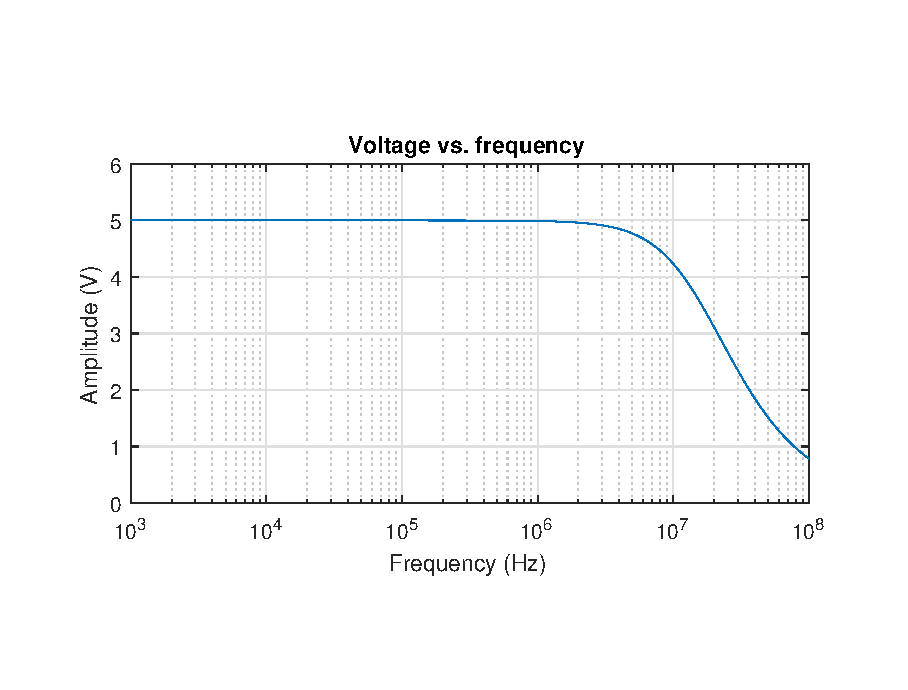
\includegraphics[trim={0cm 1.2cm 0cm 2cm},clip,width=0.8\textwidth]{img/LimiterTransfer.eps}
    \caption{$I_1$=50A}
    \label{fig:limitertransfer}
\end{figure}


%%%%%% Stikkord
%The output from the rectifiers is then again loaded down with 100 ohms.  This 100 ohms is to keep the impedance at the comparator (U6) input low, making it somewhat noise immune.  This technique works very well, and without the 100 ohm resistor in place, I find the circuit will falsely trigger on noise.  C15 provides extra noise filtering.


\newpage
\section{Power Amplifier}
\label{sec:pa}

The purpose of the power amplifier is to amplify the signal coming from the interrupter $X5$ and drive the resonant circuit with a high voltage VCC\_HVDC (\cref{sec:psu}). The power amplifier is shown in \cref{fig:tk531}, note that the feedback transformer L4, as well as the secondary resonant circuit L2 and C2 is not shown for simplicity. The feedback transformer L3 is included in the figure.

The power amplifier is a full bridge inverter using Isolated Gate Bipolar Transistors (IGBTs), IGBTs are chosen over MOSFETs due to IGBTs having lower forward voltage drop at higher voltages and currents. The IGBTs are Q1 - Q4.The 1N4744A diodes (15V Zener) is there to clamp the gate voltage to protect the gate of the IGBT from over voltage. The 10 Ohm resistors is to protect from overcurrent. The 1V5KE400A schottky diodes are to protect the IGBTs from reverse voltage transients. The 15ETX06 diodes are there to recycle the leftover energy into the bus capacitors in the power supply when we have stopped switching, as IGBTs does not conduct reverse current. L3 is the current sense feedback transformer, L1 and C1 is the primary resonant circuit. T1 and T2 are gate drive transformers. The supply voltage VCC\_HVDC is 160VDC.

\subsubsection{Gate drive transformers}
T1 and T2 are gate drive transformers, the purpose of which is to isolate the low voltages in the interrupter from the higher voltages in the power amplifier, as well as to switch the phase for half of $X5$ the signal driving the transistors.

%%%%%%% Stikkord
%the anti-parallel diodes in the IGBT recycles the leftover energy into the main bus capacitors as the current rings down.

\begin{figure}[H]
    \centering
    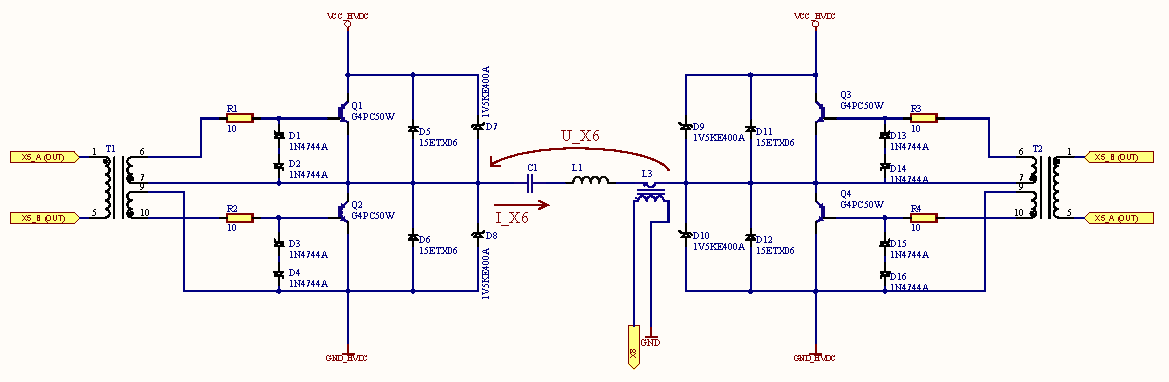
\includegraphics[width=0.9\textheight,angle=-90]{Skjema/TK531_Utgangstrinn_r.pdf}
    \caption{Power Amplifier}
    \label{fig:tk531}
\end{figure}

\newpage
\section{Coil rig}
\label{sec:resonant}

The coil rig steps up the voltage from VCC\_HVDC to a voltage high enough to create electric arcs. The coil rig consists of two parts; the primary resonant circuit; $R_1$, $C_1$, $L1$, and the secondary resonant circuit; $L_2$, $R_2$, $C_2$, $G_1$. The resonant circuit is shown in \cref{fig:spolerigg1}. The transfer function for the coil rig will be derived in \cref{sec:coilrigmath}.

\begin{figure}[H]
    \centering
    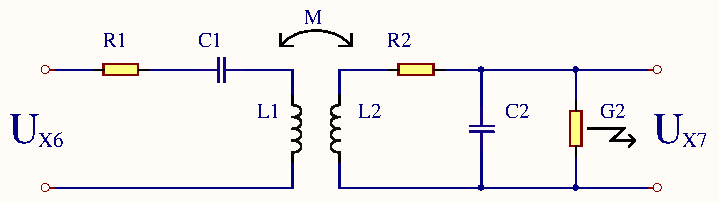
\includegraphics[width=\textwidth]{Skjema/Spolerigg1_r.pdf}
    \caption{Resonant circuit}
    \label{fig:spolerigg1}
\end{figure}

The input signal to the resonant circuit $X6$ is the square wave output from the power amplifier. When the interrupter first applies a voltage to the primary resonant circuit through the power amplifier the circuit responds with its step response on the output $U_{X7}$ and current $I_1$ (shown in \cref{fig:step} and \cref{fig:fb_step}), this is a damped sinusoidal and with a frequency equal to the resonant frequency. When the interrupter detects that the current in the primary resonant circuit $I_1$ passes zero the polarity switches, as explained in \cref{sec:interrupter}, and we get a new step response added to the already existing one. This continues for several cycles. This current is inductively coupled into the secondary resonant circuit, and when the voltage reaches a high enough level an electric discharge happens from the top load of the secondary resonant circuit, this drains energy from the secondary circuit, but the electric discharge continues to grow for a couple of cycles. The wave forms of the signals will be explained in \cref{sec:math}.

The values and the physical shapes of the components in the resonant circuit are important to the operation of the tesla coil. The values of the components will be discussed in \cref{sec:math}. A photo of a coil rig is shown in \cref{fig:foto:coilrig}.

\begin{figure}
    \centering
    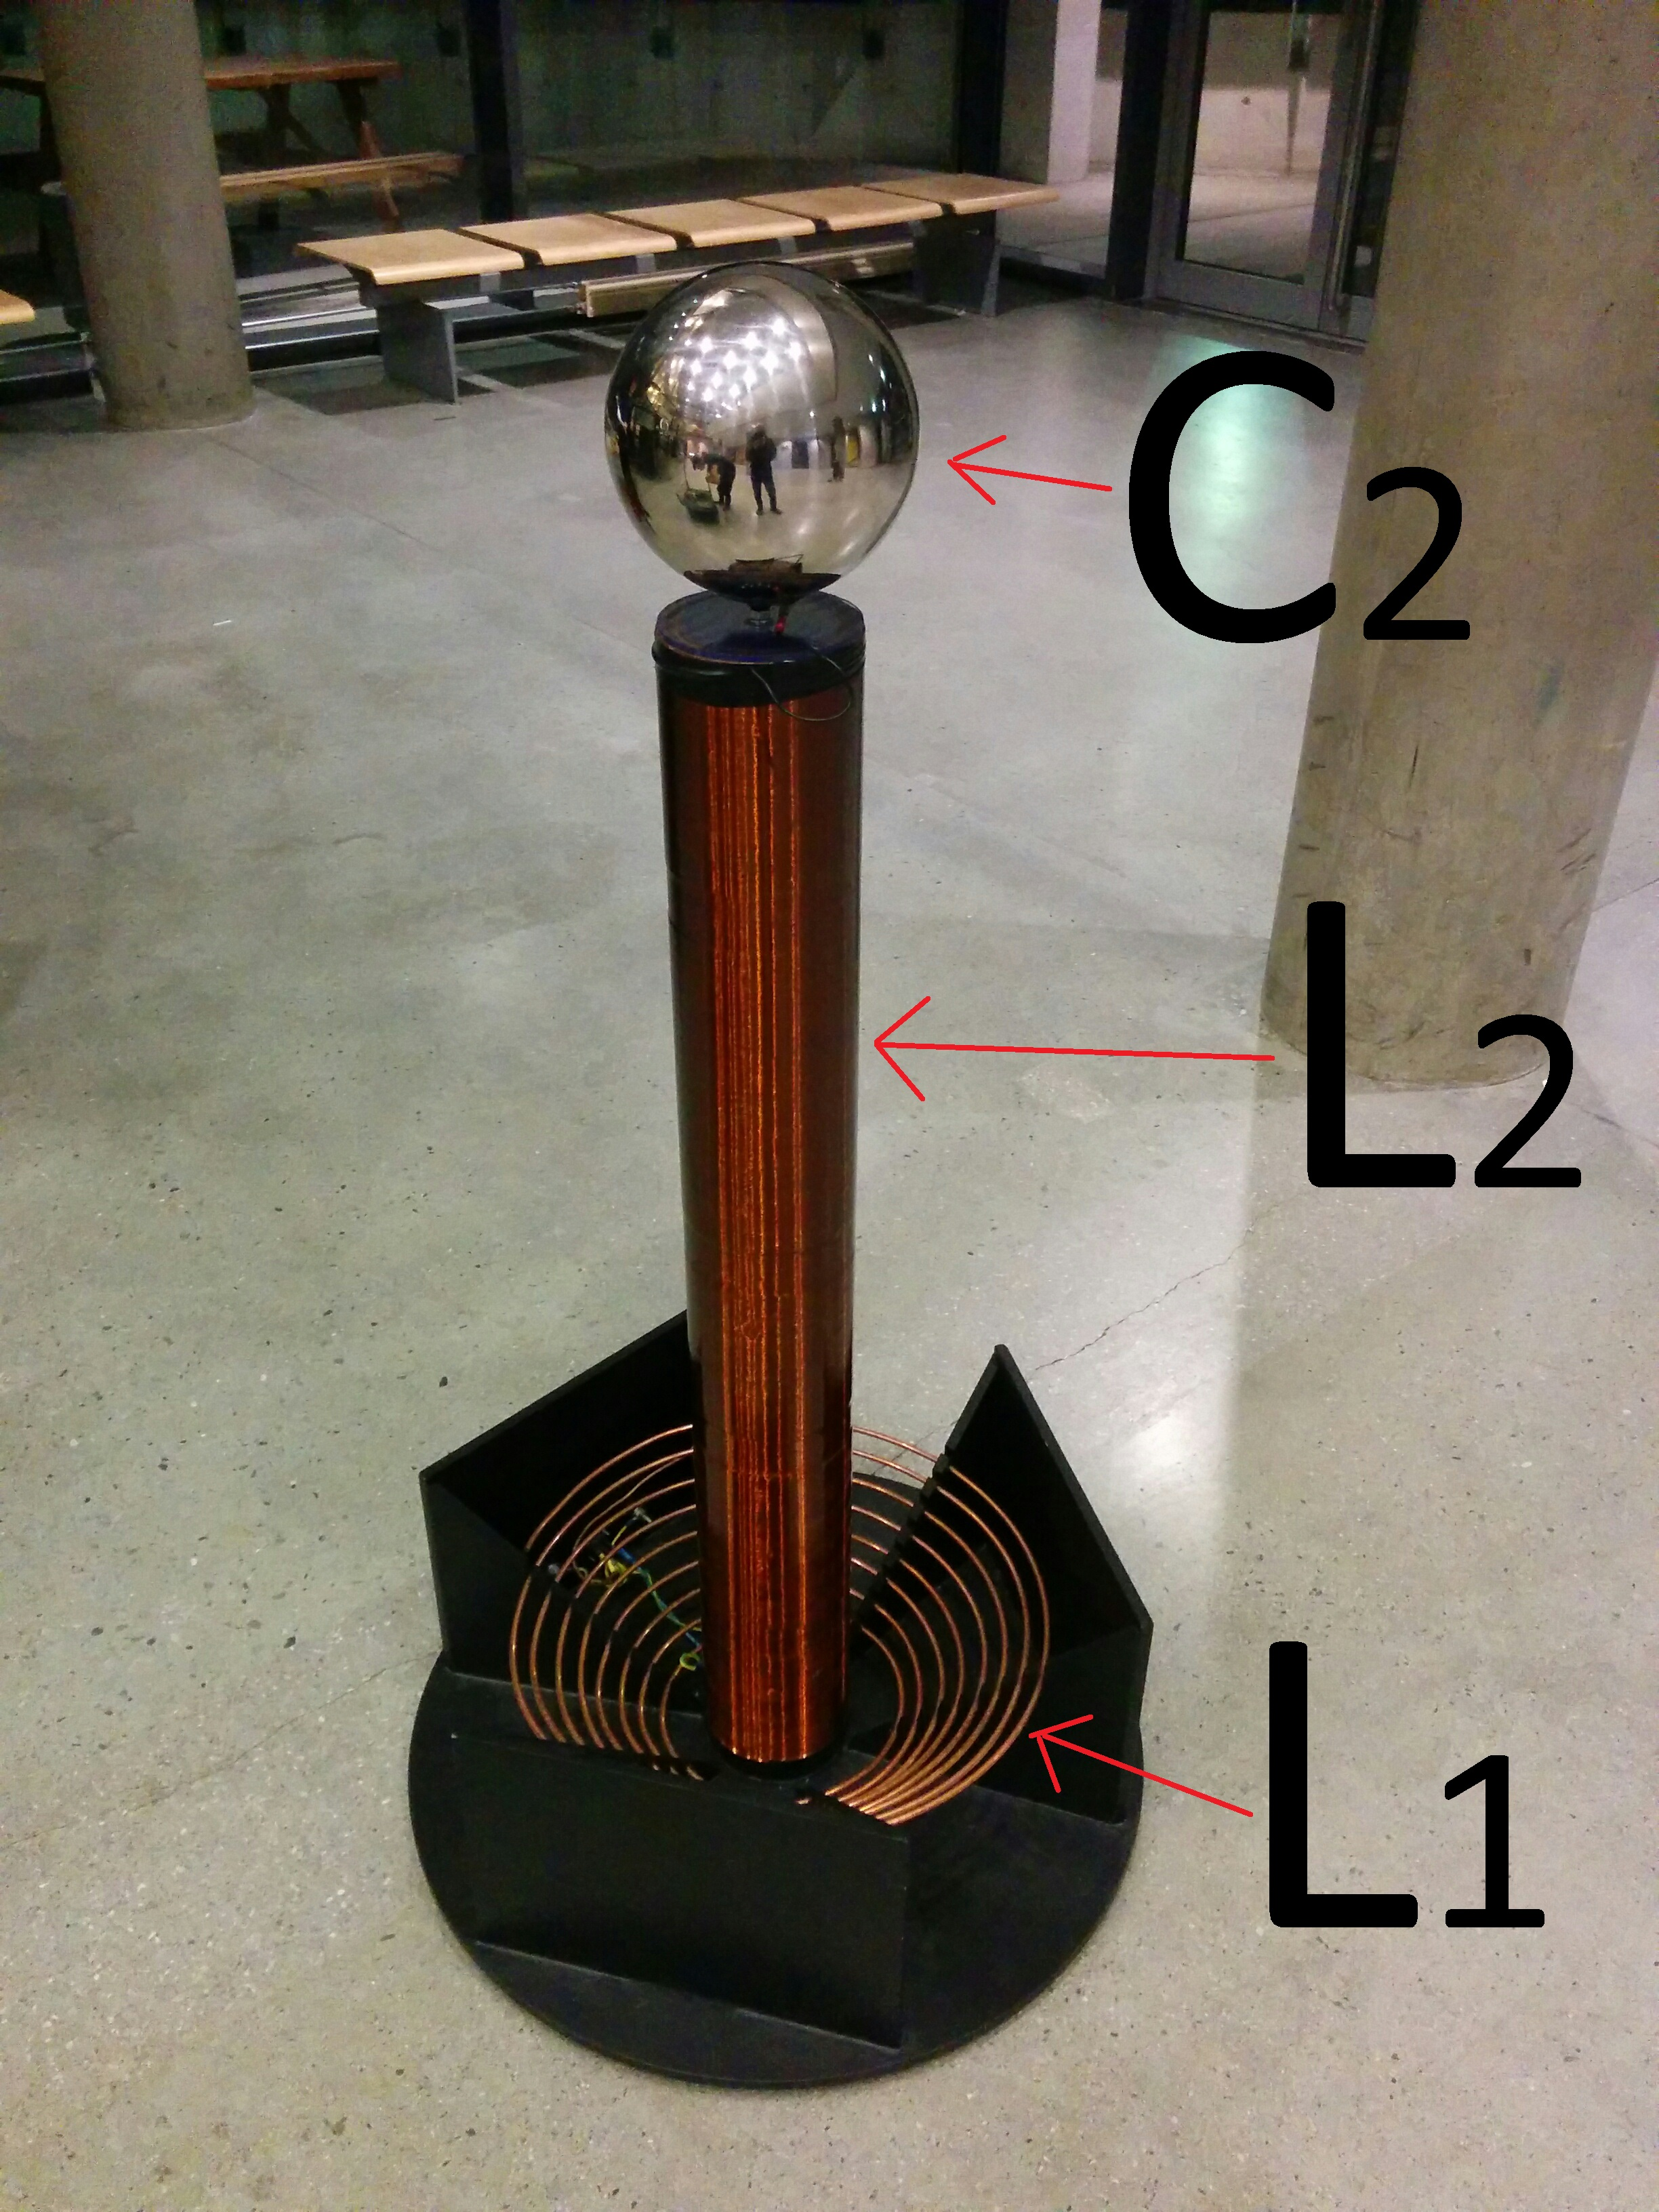
\includegraphics[width=\textwidth]{img/foto/IMG_20170201_172204.jpg}
    \caption{Image of a coil rig}
    \label{fig:foto:coilrig}
\end{figure}

$L_1$ is the primary coil, and will have few turns and large area. It is important that $L_1$ is constructed such that $k$ is $~0.2$ and so that we wont get any arcing from $L_1$ to $L_2$. This can be achieved by using a conical coil or a flat spiral coil (in \cref{fig:foto:coilrig} a conical coil is shown). The inductance of $L_1$ can be calculated from \cref{eq:l1_1} and \cref{fig:coil_l2} if a conical coil is used.

\begin{figure}
\centering
    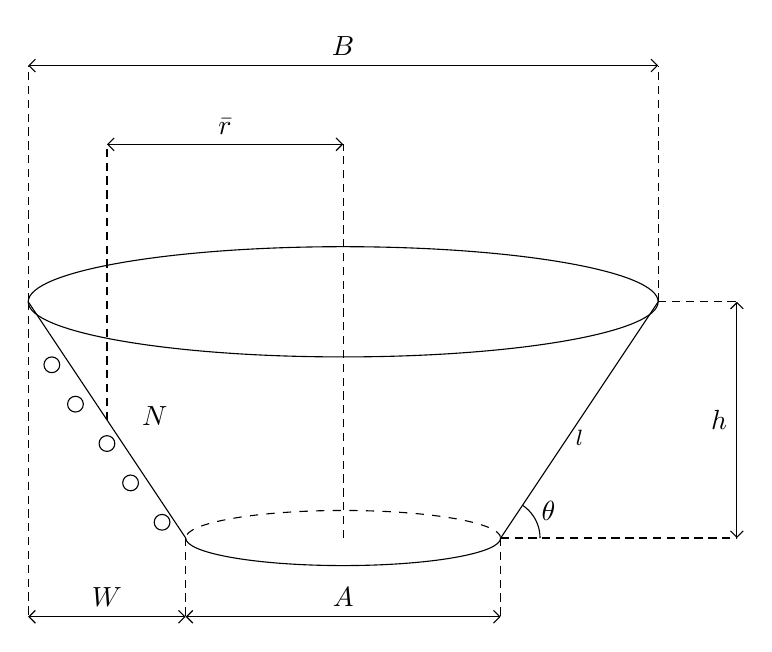
\begin{tikzpicture}[every edge/.style = {draw, Straight Barb-Straight Barb}]
        \begin{scope}
         \clip (-2,0) rectangle (2,1cm);
         \draw[dashed] (0,0) circle(2cm and 0.35cm);
        \end{scope}
        \begin{scope}
         \clip (-2,0) rectangle (2,-1cm);
         \draw (0,0) circle(2cm and 0.35cm);
        \end{scope}
        \draw (0,3) circle(4cm and 0.7cm);
        \draw (-2,0) -- (-4,3);
        \draw (2,0) -- node[below,font=\footnotesize] {$l$}coordinate[pos=0.1] (bb) (4,3);
        %%%%%
        \draw[densely dashed] (2,0) -- (5,0);
        \draw[densely dashed] (4,3) -- (5,3);
        \draw   (5,0) edge ["$h$"] (5,3);
        %%%%%
        \draw[densely dashed] (-4,3) -- (-4,-1);
        \draw[densely dashed] (-2,0) -- (-2,-1);
        \draw[densely dashed] (2,0) -- (2,-1);
        \draw (-2,-1) edge ["$A$"] (2,-1);
        \draw (-4,-1) edge ["$W$"] (-2,-1);
        %%%%%
        \draw[densely dashed] (-4,3) -- (-4,6);
        \draw[densely dashed] (4,3) -- (4,6);
        \draw (-4,6) edge ["$B$"] (4,6);
        %%%%%
        \draw[densely dashed] (-3,1.5) -- (-3,5);
        \draw[densely dashed] (0,0) -- (0,5);
        \draw (-3,5) edge ["$\bar{r}$"] (0,5);
        %%%%%
        \begin{scope}
        \path[clip] (5,0) -- (2,0) -- (4,3);
        \draw (2,0) circle (5mm);
        \node at ($(2,0)+(30:7mm)$) {$\theta$};
        \end{scope}
        \draw (-2.3,0.2) circle (1mm);
        \draw (-2.7,0.7) circle (1mm);
        \draw (-3.0,1.2) circle (1mm);
        \draw (-3.4,1.7) circle (1mm);
        \draw (-3.7,2.2) circle (1mm);
        \node at ($(-3,1.2)+(30:7mm)$) {$N$};
    \end{tikzpicture}
    \caption{Conical coil}
    \label{fig:coil_l2}
\end{figure}


\begin{equation} \label{eq:l1_1}
    L_1 = \sqrt{(L_{1V}\cdot \sin (\theta))^2 + (L_{1H}\cdot \cos (\theta))^2}
\end{equation}

\begin{equation} \label{eq:l1_2}
    L_{1V} = \frac{R^2 N^2}{9 \bar{r} + 10 h}, L_{1H} = \frac{R^2 N^2}{8 \bar{r} + 11 h}
\end{equation}

\begin{equation} \label{eq:l1_3}
    \bar{r} = \frac{A}{2} + \frac{W}{2}
\end{equation}

\begin{equation} \label{eq:l1_4}
    \sin (\theta) = \frac{h}{l}, \cos (\theta) = \frac{W}{l}
\end{equation}

\begin{equation} \label{eq:l1_5}
    l = \sqrt{W^2 + h^2}
\end{equation}

\begin{equation} \label{eq:l1_6}
    W = \frac{B - A}{2}
\end{equation}

% Harold A. Wheeler, "Simple Inductance Formulas for Radio Coils," Proceedings of the I.R.E., October 1928, pp. 1398-1400

$h$ is height of cone, $B$ diameter top of cone, $A$ diameter base of cone, $N$ number of turns, $\bar{r}$ is effective with of coil $l$ is length of coil, $\theta$ is angle of coil, $L_{1V}$ is the vertical component of the inductance, $L_{1H}$ is the horizontal part of the inductance. This equation comes from the empirical wheeler equations \citep{wheeler}.

$L_2$ is the secondary coil and will have many turns and small area. This has the form of a solenoid with a single layer of windings. The inductance of $L_2$ can be found with \cref{eq:l2}.

\begin{equation} \label{eq:l2}
    L_2 = \frac{{\mu}_0 N^2 \pi {r}^2}{l}
\end{equation}

Where ${\mu}_0$ is permeability for vacuum, $N$ is the number of turns, and $l$ is the length of the coil. This equation comes from the long solenoid approximation.

$C_1$ is an ordinary capacitor, the type of capacitor should be chosen to withstand the voltages and current required without degrading. And should have as low resistance as possible.

$C_2$ is the place where we want the electric discharge to happen, and thus $C_2$ must withstand the voltages and currents required without degrading. This is achieved by using the self capacitance of a single conductor as opposed to the more common mutual capacitance of two paralell plates. $C_2$ is placed at the top of $L_2$ and is also known as the top load, the top load can be any shape that does not have sharp corners. The most common shapes are spherical or toroidal. The self capacitance of a spherical top load $C_2$ is given by \cref{eq:c2}.

\begin{equation} \label{eq:c2}
    C_2 = 4 \pi {\epsilon}_0 r_{c}
\end{equation}

Where ${\epsilon}_0$ is the permittivity of vacuum, and $r_c$ is the radius of the sphere. This equation is derived from the capacitance of an spherical paralell plate capacitor where the radius of the outer sphere goes toward infinity.

%%%%%%%%%%%%% Stikkord
% Løs kobling mellom primær og sekundær for å ikke laste primærkretsen for mye.
% Må tune primær til samme frekvens som sekundær
% Sekundær bestemmer frekvensen.
% Q verdi?
%$C_1$ is a bank of capacitors with high voltage and current rating and low equivalent series resistance (ESR). $L_1$ is an inductor with high cross section area and few turns (in the magnitude of 5 turns). $L_2$ is an inductor with low cross section area and a high number of turns (in the magnitude of 4000 turns). $C_2$ consists of a sphere or toroid for one plate, and the grounded (safety ground) surroundings. Ground is connected through the safety ground in the electrical socket used to power the DRSSTC. $L_3$ and $L_4$ are current sensing transformers used for feedback.

\section{Power supply}
\label{sec:psu}
The power supply for the driver is, as for most electronic systems, critical for the quality of operation. This implementation uses three different power supplies for VCC\_P5V0, VCC\_P18V, and VCC\_HVDC. Wich are 5,0V DC, 18V DC, and 160V DC respectively. VCC\_P5V0 supplies the logic circuits, and should supply enough power for this, as well as not introducing noise to the signals in the logic circuits. VCC\_P18V supplies power to the transistor drivers in the interrupter, and has the same requirements as VCC\_P5V0. VCC\_HVDC supplies the power amplifier, and should be able to supply large peak currents with low resistance and delay, as seen from the simulation of the current drawn by the primary resonant circuit in \cref{fig:fblinsim} in \cref{sec:mod_fb}. How this can be achieved is assumed well understood and documented in the field of electronics and will not be discussed any further.

\section{Shielding}
\label{sec:shielding}
The electric discharge produced by a tesla coil generates a large dynamic electromagnetic field. This will induce currents in any conductor close to the tesla coil. This must be taken into account when doing pcb layout and designing the chassis for the tesla coil driver. How this can be achieved is assumed well understood and documented in the field of electronics and electrodynamics and will not be discussed any further.

\section{Optical channel}
\label{sec:optical}

As mentioned in \cref{sec:shielding} there is electromagnetic noise present when the tesla coil is used and a robust channel is needed for signal $X2$ because this signal is transmitted from the pulse shaper to the tesla coil driver, wich as mentioned in \cref{sec:pulseshaper} are physically located in different chassis some distance apart. For this plastic optical fibre is chosen. To further increase the robustness the signal $X2$ is modulated. The robustness and possible noise introduced in this channel is not discussed further as it can be treated as an isolated problem and is assumed well understood and documented in the field of electronics. A diagram of the optical channel is shown in \cref{fig:opticalchannel}.

\begin{figure}[H]
    \centering
    \tikzstyle{int}=[draw, fill=yellow!20, minimum size=2em]
    \tikzstyle{init} = [pin edge={to-,thin,black}]
    \begin{tikzpicture}[node distance=2.5cm,auto,>=latex']
        \node [int, pin={[init]above:$CW$}] (a) {tx};
        \node (b) [left of=a,node distance=2cm, coordinate] {a};
        \node [int] (c) [right of=a] {rx};
        \node [int] (d) [left of=a] {Pulse shaper};
        \node [int] (e) [right of=c] {Interrupter};
        \node [coordinate] (end) [right of=c, node distance=2cm]{};
        \path[->] (d) edge node {$X2$} (a);
        \path[->] (a) edge node {$PWM$} (c);
        \draw[->] (c) edge node {$X2$} (e) ;
    \end{tikzpicture}
    \caption{Diagram of optical channel}
    \label{fig:opticalchannel}
\end{figure}

Where CW is the carrier wave used to modulate the signal $X2$, PWM is the modulated signal $X2$. The blocks tx and rx are the optical transmitter and reciever.
%Inngående beskrivelse av signaler i kretsene
%\section{Signals in the DRSSTC}
A description of the different signals in the DRSSTC

\subsection{Triggering signal (X2)}
\label{triggering_signal}
The triggering signal $X2$ is two level and contains two pieces of information from $X1$, the frequency $f$ (tone) and the volume (intensity). The frequency is given by the time $T$ between the positive flanks of the signal $f=\frac{1}{T}$. This is the base harmonic of the acoustic tone heard at the output of the system. The volume is given by the duty cycle of the pulses (the relationship between the pulse being high and the total period $T$ of the pulse. \Cref{fig:tones} shows different tones, and \cref{fig:volumes} shows different volumes.

\begin{figure}[!ht]
    \centering
    \begin{tikztimingtable}
        X2 & 2L 1H 7L 1H 7L 1H 7L 1H 7L\\
        X2 & 2L 1H 5L 1H 5L 1H 5L 1H 5L 1H 5L 1H 1L\\
    \end{tikztimingtable}
    \caption{Different tones}
    \label{fig:tones}
\end{figure}{}

\begin{figure}[!ht]
    \centering
    \begin{tikztimingtable}
        X2 & 2L 1H 7L 1H 7L 1H 7L 1H 7L\\
        X2 & 2L 3H 5L 3H 5L 3H 5L 3H 5L\\
    \end{tikztimingtable}
    \caption{Different volumes}
    \label{fig:volumes}
\end{figure}{}

\subsection{Feedback signal (X8)}
The feedback signal X8 and X9, are coupled with a feedback transformer to the primary resonant circuit. The feedback transformers are hand wound 100 turns around a ferrite toroid wich the wire in the resonant circuit is fed trough. If this transformer is loaded with a transistor we will get a voltage over the transistor dependent on and in phase with the current running in the primary resonance circuit. The current running 

\subsection{Primary resonant circuit signal (X6)}

\subsection{Secondary resonant circuit signal (X7)}
%Matematisk beskrivelse av så mye som mulig av kretsen(e)
\chapter{Mathematical model}
\label{sec:math}


\section{Transfer function for coil rig}

The schematic shown in \cref{fig:spolerigg11} is the schematic for the coil rig.

\begin{figure}[h!]
    \centering
    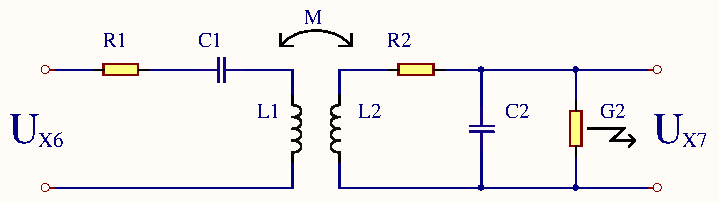
\includegraphics[width=\textwidth]{Skjema/Spolerigg1_r.pdf}
    \caption{Caption}
    \label{fig:spolerigg11}
\end{figure}

R1 is the resistance in the primary circuit (mainly the cable from the driver to the coil rig), R2 is the resistance in the secondary circuit (mainly the resistance in L2). C1 is the primary capacitor, L1 is the primary coil, L2 is the secondary coil, and C2 is the secondary capacitance (or top load). G1 is the electrical arc modelled as a conductance, see \cref{eq:g1} for the model of G1, this model is a combination of Cassie \citep{cassie} and Mayr \citep{mayr} models for electrical arcs presented in \citep{575670}. $U_{X6}$ is the voltage output from the driver to the primary resonant circuit, $U_{X7}$ is the voltage output from the secondary resonant circuit (the voltage driving the electrical arc).

This schematic can be simplified by introducing the mutual inductance M as a component as shown in \cref{fig:spolerigg2}, and then further simplified by representing the branches of the circuit as impedances as shown in \cref{fig:spolerigg3}.

\begin{figure}[h!]
    \centering
    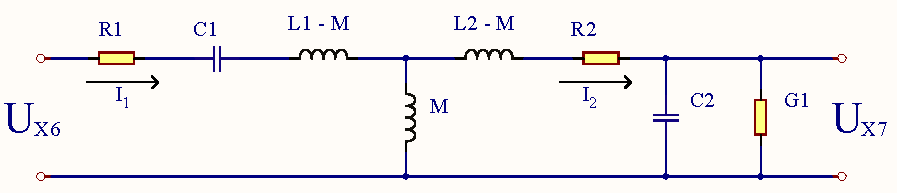
\includegraphics[width=\textwidth]{Skjema/Spolerigg2_r.pdf}
    \caption{Caption}
    \label{fig:spolerigg2}
\end{figure}

\begin{figure}[h!]
    \centering
    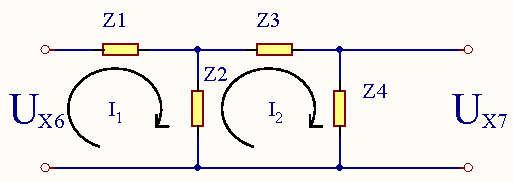
\includegraphics[width=\textwidth]{Skjema/Spolerigg3_r.pdf}
    \caption{Caption}
    \label{fig:spolerigg3}
\end{figure}

Using the mesh current method we get \cref{eq:1} and \cref{eq:2}.

\begin{equation} \label{eq:1}
    U_{X6} - I_1 Z_1 - (I_1 - I_2) Z_2 = 0
\end{equation}

\begin{equation} \label{eq:2}
    (I_2 - I_1) Z_2 - I_2 Z_3 - I_2 Z_4 = 0
\end{equation}

We then solve these two equations for $I_1$. Set \cref{eq:1_2} equal to \cref{eq:2_2}, solve for $\frac{U_{X7}}{U_{X6}}$ and substitute in \cref{eq:3}.

\begin{equation} \label{eq:3}
    U_{X7} = I_2 Z_4
\end{equation}

\begin{equation} \label{eq:1_2}
    I_1 = \frac{U_{X6} + I_2 Z_2}{Z_1 + Z_2}
\end{equation}'

\begin{equation} \label{eq:2_2}
    I_1 = \frac{(Z_2 - Z_3 - Z_4) I_2}{Z_2}
\end{equation}

We then have the transfer function $H(s)$ for the coil rig \cref{eq:4}.

\begin{equation} \label{eq:4}
    \frac{U_{X7}}{U_{X6}} = H(s) = \frac{Z_2 \cdot Z_4}{Z_1 \cdot (Z_2 - Z_3 - Z_4) - Z_2 \cdot (Z_3 + Z_4))}
\end{equation}

where

\begin{equation} \label{eq:4_1}
    Z_1 = R_1 + \frac{1}{s C_1} + s L_1 - s M,
\end{equation}

\begin{equation} \label{eq:4_2}
    Z_2 = s M,
\end{equation}

\begin{equation} \label{eq:4_3}
    Z_3 = s L_2 - s M + R_2,
\end{equation}

\begin{equation} \label{eq:4_4}
    Z_4 = \frac{1}{s C_2} + \frac{1}{G_1},
\end{equation}

\begin{equation} \label{eq:4_5}
    M = k \sqrt{L_1 L_2}.
\end{equation}

%\begin{equation}
%    H(s) = \frac{s M (\frac{1}{s C_2} + \frac{1}{G_1})}{(R_1 + \frac{1}{s C_1} + s L_1 - s M) \cdot (s M - (s L_2 - s M + R_2) - (\frac{1}{s C_2} + \frac{1}{G_1})) - s M \cdot ((s L_2 - s M + R_2) + (\frac{1}{s C_2} + \frac{1}{G_1})))}
%\end{equation}

% (Z2*Z4)/(Z1*(Z2-Z3-Z4)-Z2*(Z3+Z4)), Z1=(R1+1/(s*C1)+s*L1-s*M), Z2=(s*M, Z3=(s*L2)-(s*M)+R2), Z4=(1/(s*C2))+(1/G1))
However to be able to analyze this transfer function we have to order it into standard form. Meaning isolating $s$,$s^2$,$s^3$ etc. and expanding the factors. This leads to \cref{eq:5}.

%\begin{equation}
%    H(s) = \frac{s^2 M C_1}{s^4(2 M L_1 C_2 C_1 - L_1 L_2 C_2 C_1) + s^3(2 M R_1 C_2 C_1 - L_2 R_1 C_2 C_1 + 2 M L_1 G_1 C_1 - L_1 R_2 C_2 C_1) + s^2(2 M R_1 G_1 C_1 - R_1 R_2 C_2 C_1 + 2 M C_2 - C_2 L_2 - L_1 R_2 G_1 C_1 - L_1 C_1 + 2 M C_1) + s(2 M G_1 - R_1 R_2 G_1 C_1 - R_1 C_1 - L_2 G_1) - R_2 G_1- 1}
%\end{equation}

\begin{equation} \label{eq:5}
    H(s) = \frac{s^3 f + s^2 g}{s^4 a + s^3 b + s^2 c + s d + e}
\end{equation}

where

\begin{equation} \label{eq:5_1}
    a = (C_1 C_2 G_1 L_1 L_2)-2 (C_1 C_2 G_1 L_1 M)+(C_1 C_2 G_1 M^2),
\end{equation}

\begin{equation} \label{eq:5_2}
    b = (C_1 C_2 G_1 L_1 R_2)+(C_1 C_2 G_1 L_2 R_1)-2 (C_1 C_2 G_1 M R_1)+(C_1 C_2 L_1),
\end{equation}

\begin{equation} \label{eq:5_3}
    c = (C_1 C_2 G_1 R_1 R_2)+(C_1 C_2 R_1)+(C_1 G_1 L_1)+(C_2 G_1 L_2)-2 (C_2 G_1 M),
\end{equation}

\begin{equation} \label{eq:5_4}
    d = (C_1 G_1 R_1)+(C_2 G_1 R_2)+C_2,
\end{equation}

\begin{equation} \label{eq:5_5}
    e = G_1,
\end{equation}

\begin{equation} \label{eq:5_6}
    f = C_1 C_2 M,
\end{equation}
and
\begin{equation} \label{eq:5_7}
    g = C_1 G_1 M.
\end{equation}

Orders of magnitude for the parameters in the transfer function is shown in \cref{tab:mod_params} these sizes are rounded approximate sizes for a DRSSTC.

\begin{table}[]
    \centering
    \begin{tabular}{c|c|c|c}
         & Comment &  &\\ \hline
        C1 & Primary load capacitor                 & $10^{-7}$ & F \\
        C2 & Secondary load capacitor (top load)    & $10^{-11}$& F \\
        L1 & Primary coil                           & $10^{-5}$ & H \\
        L2 & Secondary coil                         & $10^{-1}$ & H \\
        M  & Mutual inductance                      & $10^{-6}$ & H \\
        R1 & Primary circuit ohmic resistance       & $10^{1}$  & $\Omega$ \\
        R2 & Secondary circuit ohmic resistance     & $10^{2}$  & $\Omega$ \\
        G1 & Conductance of elecrical arc           & $10^{-6}$  & $\Omega$ \\
        k  & Coupling factor                        & $10^{-1}$ & 
    \end{tabular}
    \caption{Model parameter sizes}
    \label{tab:mod_params}
\end{table}

\todo{Forklare hvorfor disse størrelsene}

Shown in \cref{fig:bode} is the bode plot of the transfer function $H(j\omega)$ \cref{eq:5} of the resonant circuit with the orders of magnitude in \cref{tab:mod_params}.

\begin{figure}[H]
    \centering
    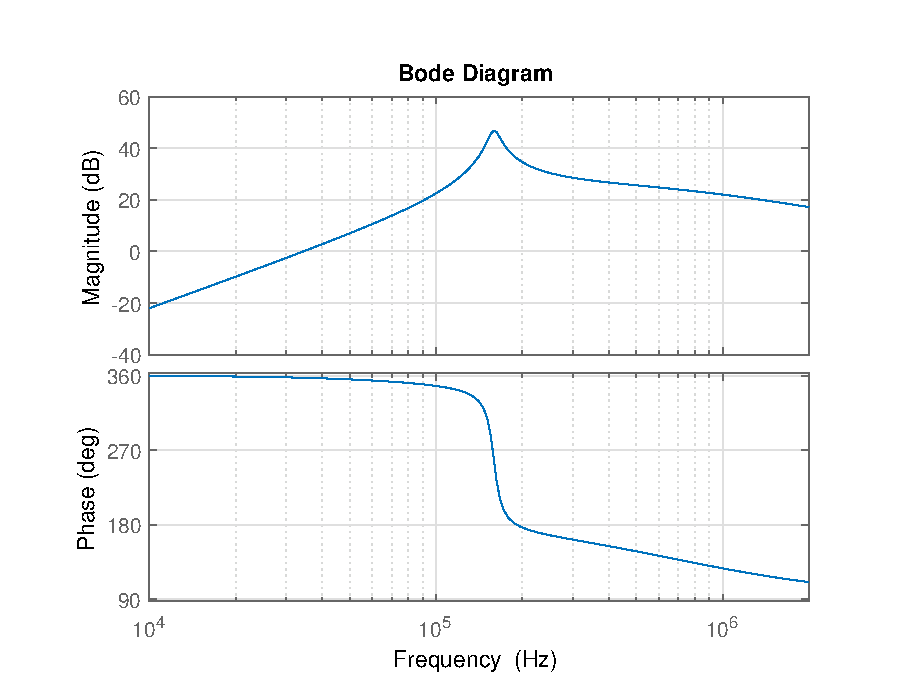
\includegraphics[width=\textwidth]{img/CoilRigBode.eps}
    \caption{Bode plot of $H(j\omega)$}
    \label{fig:bode}
\end{figure}

Here we see that the frequency response takes the form of a resonant circuit with a resonant frequency $f_0$ of 157kHz, which is close to the frequency one would expect with the orders of magnitude given in \cref{tab:mod_params} and the equation for resonance frequency \cref{eq:f0} of 160kHz. The magnitude at resonance is 36,7dB and then flattens at a magnitude 26dB at frequencies higher than resonance.

\begin{equation} \label{eq:f0}
    f_0 = \frac{1}{2 \pi \sqrt{L_1 C_1}}
\end{equation}

\todo{Skriv om å variere parametre}
\todo{Varier G1 fra 1e-5 til 1e-6}

In \cref{fig:step}, we see the step and impulse responses of the transfer function $H(j\omega)$ for the resonant circuit.

\begin{figure}[H]
    \centering
    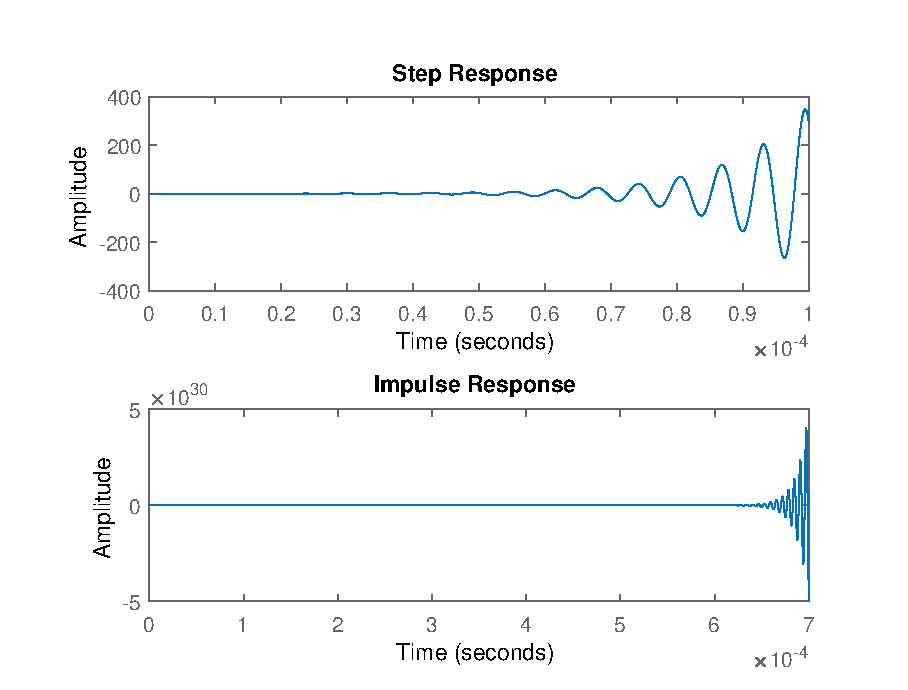
\includegraphics[width=\textwidth]{img/CoilRigResponse.eps}
    \caption{Step and impulse response for $H(j\omega)$}
    \label{fig:step}
\end{figure}

Here we see that we have a damped sinusiodal response with a frequency $f_s$ of 156kHz witch is the same frequency as the resonance frequency $f_0$ of the frequency response. This response attenuates within a few cycles.

\Cref{fig:polezero} shows the poles and zeros of the transfer function $H(j\omega)$ of the resonant circuit.

\begin{figure}[H]
    \centering
    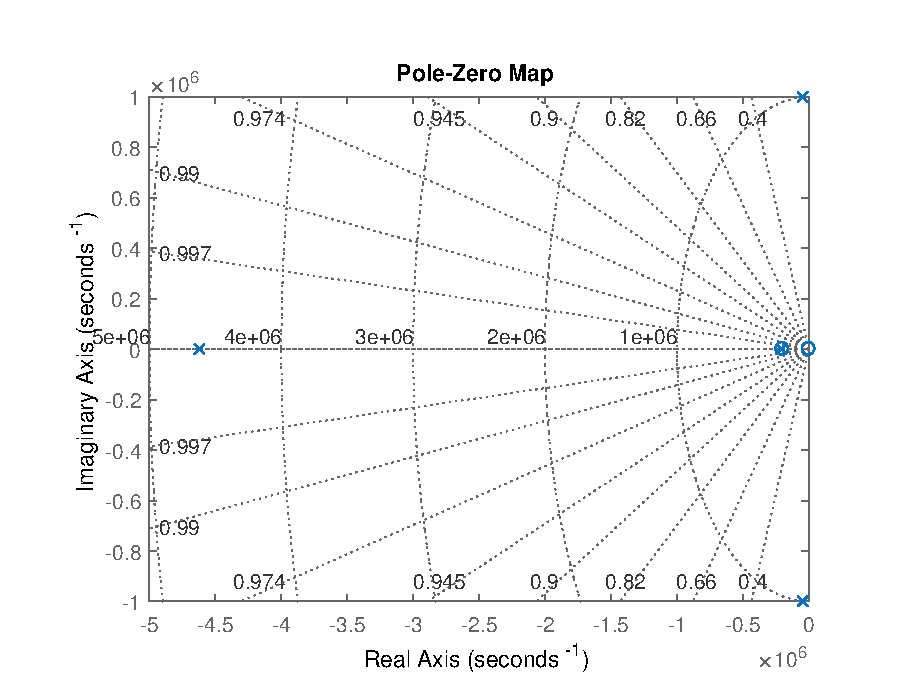
\includegraphics[width=\textwidth]{img/CoilRigPoleZeroPlot.eps}
    \caption{PoleZeroPlot for $H(j\omega)$}
    \label{fig:polezero}
\end{figure}

\Cref{tab:coilrigpoles} shows the numerical values of the poles and zeros of the transfer function $H(j\omega)$ of the resonant circuit.

\begin{table}[h]
    \centering
    \begin{tabular}{c|c}
        Poles & Zeros \\
        $(-1,4 + 9,6i)\cdot 10^{5} s^{-1}$ & $0$ \\
        $(-1,4 - 9,6i)\cdot 10^{5} s^{-1}$ & $0$ \\
        $(-2,1 + 0i)\cdot 10^{5} s^{-1}$ & $-2\cdot 10^{5} s^{-1}$ \\
    \end{tabular}
    \caption{Poles and zeros for $H(j\omega)$}
    \label{tab:coilrigpoles}
\end{table}

Here we observe a pole pair in the left half plane, a single real pole in the left half plane. As well as three zeros, one in the left half plane and two in origo.

\Cref{fig:crlinsim} shows the result of a linear simulation of the transfer function of the resonant circuit with a 160V peak square wave input signal with amplitude 1 and frequency 159kHz.

\begin{figure}[H]
    \centering
    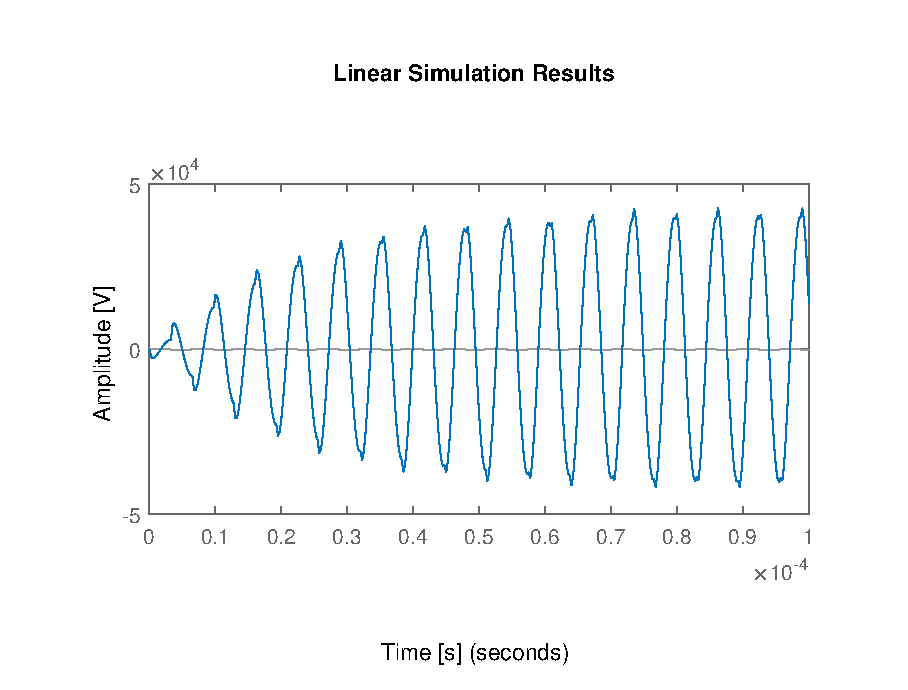
\includegraphics[width=\textwidth]{img/CoilRigSimulation.eps}
    \caption{Linear simulation of transfer function with square wave with $f=f_0$ as input}
    \label{fig:crlinsim}
\end{figure}

We see here that the output signal X6 starts with a quarter period of the step response shown in \cref{fig:step}, and then when the voltage peaks, meaning when the differential of the voltage is zero, a new step response with opposite phase is added to the output signal. This makes the output signal grow rapidly for three cycles to 160kV, before flattening out at 170kV.

\Cref{fig:crlinsim10T} shows the same simulation as \cref{fig:crlinsim}, but here the input signal is set to zero after 10 periods.

\begin{figure}
    \centering
    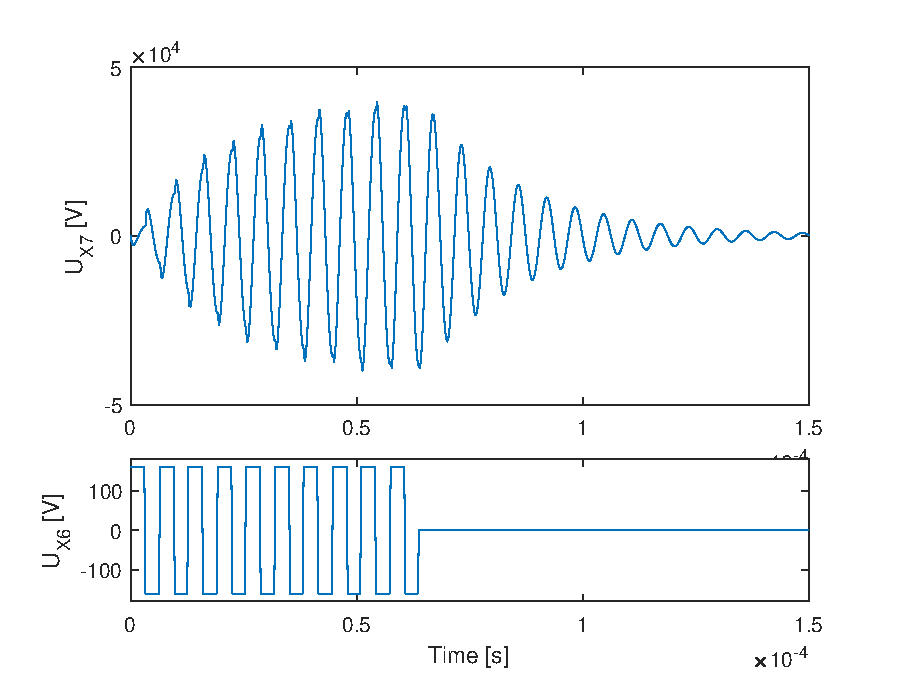
\includegraphics[width=\textwidth]{img/Linsim_10T.eps}
    \caption{Linear simulation of transfer function with square wave with 10 periods at $f=f_0$ as input}
    \label{fig:crlinsim10T}
\end{figure}

Here we see that the voltage continues to resonate after the input is set to zero, but attenuates exponentially.

\newpage
\section{Transfer function for feedback}
\label{sec:mod_fb}
If we use \cref{eq:1} and \cref{eq:2} and solve for $\frac{I_1}{U_{X6}}$ we get the transfer function for the feedback signal shown in \cref{eq:fb_1} to \cref{eq:fb_q}. Where $Z_1$ to $Z_4$ are the same impedances as given in \cref{eq:4}.

\begin{equation} \label{eq:fb_1}
\frac{I_1}{U_{X6}} = H_{FB}(s) = \frac{Z_2-Z_3-Z_4}{(Z_1+Z_2)(Z_2-Z_3-Z_4)-Z_2^2}
\end{equation}

\begin{equation} \label{eq:fb_2}
    H_{FB}(s) = \frac{s^3 h + s^2 k + s l}{s^4 m + s^3 n + s^2 o + s p + q}
\end{equation}

Where

\begin{equation}
    h = 2(C_1 C_2 G_1 M) - (C_1 C_2 G_1 L_2)
\end{equation}

\begin{equation}
    k = -(C_1 C_2 G_1 R_2) - (C_1 C_2)
\end{equation}

\begin{equation}
    l = -C_1 G_1
\end{equation}

\begin{equation}
    m = (C_1 C_2 G_1 L_1 L_2)-2(C_1 C_2 G_1 L_1 M)
\end{equation}

\begin{equation} \label{eq:fb_n}
    n = (C_1 C_2 G_1 L_1 R_2) + (C_1 C_2 L_1) + (C_1 C_2 G_1 R_1 L_2) - 2(C_1 C_2 G_1 R_1 M)
\end{equation}

\begin{equation} \label{eq:fb_o}
    o = (C_1 G_1 L_1) + (C_1 C_2 R_1) + (C_2 G_1 L_2) -2(C_2 G_1 M)
\end{equation}

\begin{equation} \label{eq:fb_p}
    p = (C_1 G_1 R_1) + (C_2 G_1 R_2) + C_2
\end{equation}

\begin{equation} \label{eq:fb_q}
    q = G_1
\end{equation}

\Cref{fig:fb_bode} Shows the bode plot for the transfer function $H_{FB}(j\omega)$ for the feedback signals X8 and X9 (both are identical).

\begin{figure}[H]
    \centering
    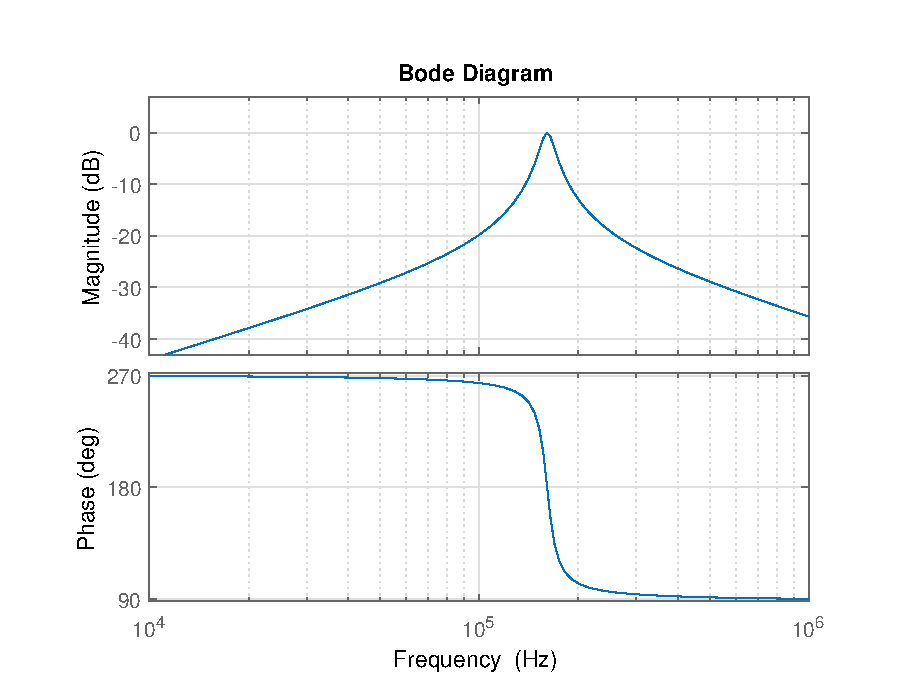
\includegraphics[width=\textwidth]{img/FeedBackBode.eps}
    \caption{Bode plot of the transfer function for the feedback signals $H_{FB}(j\omega)$}
    \label{fig:fb_bode}
\end{figure}

Here we see a much sharper peak at the resonant frequency than in the bode plot for the resonant circuit $H(j\omega)$. We also see that the response does not flatten at frequencies higher than the resonance frequency. The resonant frequency $f_0$ is 160kHz and the magnitude is 0dB at resonance.


\Cref{fig:fb_step} shows the step and impulse response of the feedback transfer function $H_{FB}(j\omega)$.

\begin{figure}[H]
    \centering
    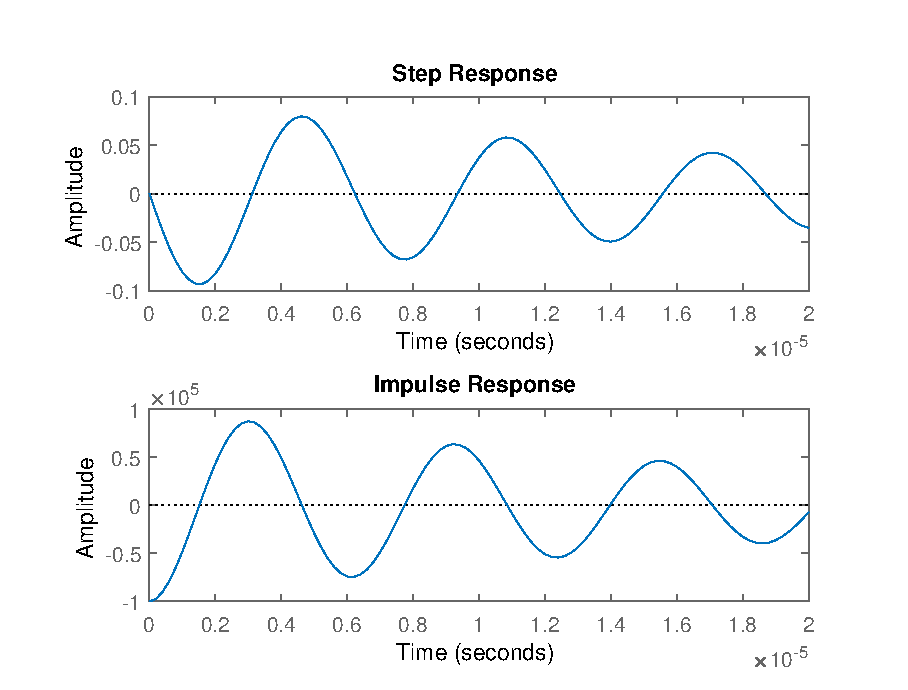
\includegraphics[width=\textwidth]{img/FeedBackResponse.eps}
    \caption{Step and impulse response of transfer function for the feedback current}
    \label{fig:fb_step}
\end{figure}

Here we see a damped sinusoiodal response with a frequency $f_s$ of 167kHz witch is slightly higher than the resonant frequency $f_0$ of 160kHz. The step response of the feedback signal attenuates slower than the step response of the resonant circuit.

\Cref{fig:fbpolezero} shows the pole and zero plot for the transfer function for the feedback signals $H_{FB}(j\omega)$.

\begin{figure}[H]
    \centering
    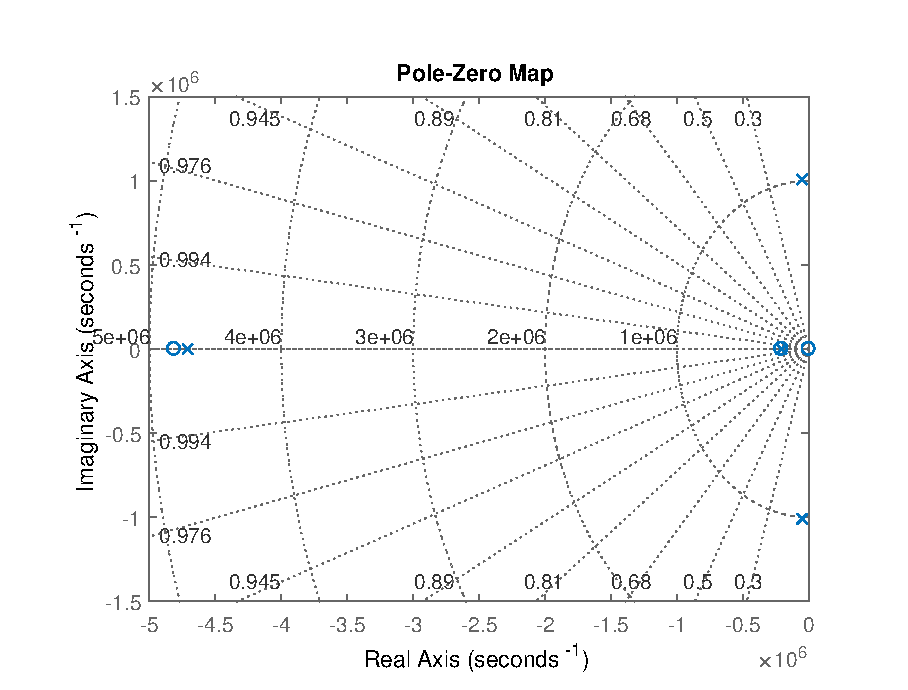
\includegraphics[width=\textwidth]{img/FeedBackPoleZeroPlot.eps}
    \caption{PoleZeroPlot for $H_{FB}(j\omega)$}
    \label{fig:fbpolezero}
\end{figure}

\Cref{tab:fbcoilrigpoles} shows the numerical values of the poles and zeros of the transfer function for the feedback signals $H_{FB}(j\omega)$.

\begin{table}[h]
    \centering
    \begin{tabular}{c|c}
        Poles & Zeros \\
        $(-47 + 0i)\cdot 10^{5} s^{-1}$ & \\
        $(-0,5 + 10i)\cdot 10^{5} s^{-1}$ & $0$ \\
        $(-0,5 - 10i)\cdot 10^{5} s^{-1}$ & $-48\cdot 10^{5} s^{-1}$ \\
        $(-2,1 + 0i)\cdot 10^{5} s^{-1}$ & $-2,1\cdot 10^{5} s^{-1}$ \\
    \end{tabular}
    \caption{Poles and zeros for $H_{FB}(j\omega)$}
    \label{tab:fbcoilrigpoles}
\end{table}

Here we observe a pole pair in the left half plane, two real poles in the left half plane. As well as three zeros, two in the left half plane and one in origo.

\Cref{fig:fblinsim} shows the result of a linear simulation of the transfer function of the feedback signal with a 160V peak square wave input signal with amplitude 1 and frequency 159kHz.

\begin{figure}[H]
    \centering
    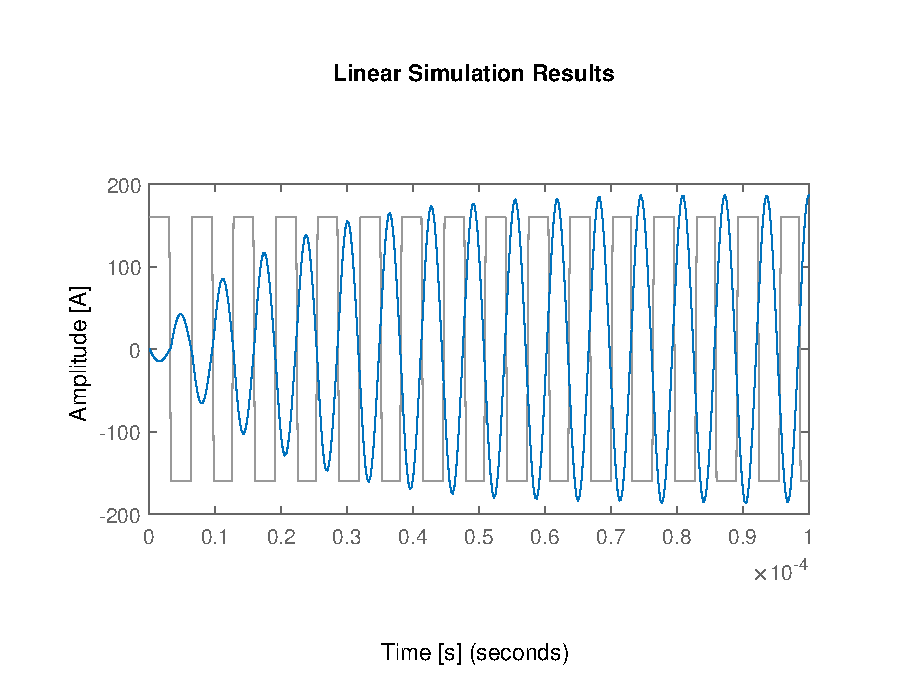
\includegraphics[width=\textwidth]{img/FeedBackSimulation.eps}
    \caption{Linear simulation of transfer function with square wave with $f=f_0$ as input}
    \label{fig:fblinsim}
\end{figure}

Here we see a sinusoidal current that grows rapidly for 9 cycles to 182A then stabilizes at 186A. We also see that the input signal switches when the current is zero, though after some cycles the input signal drifts out of sync with the current.

\newpage
\section{Magnitude analysis}
By taking the magnitudes for each variable listed in \cref{tab:mod_params} and inserting them into the different terms in the transfer function $H(s)$ (\cref{eq:4}) we can see witch terms influence the result and witch terms are insignificant. In \cref{tab:termsh} the values of each of the terms making up the main terms in \cref{eq:4}, are listed after inserting the magninudes in \cref{tab:mod_params}. e, f, and g are not listed since they only have a single term each.

\begin{table}[H]
    \centering
    \begin{tabular}{c|c|c}
        a & $(C_1 C_2 G_1 L_1 L_2)$   & $2 \cdot 10^{-29}$ \\
          & $2 (C_1 C_2 G_1 L_1 M)$   & $8 \cdot 10^{-32}$ \\
          & $(C_1 C_2 G_1 M^2)$       & $8 \cdot 10^{-31}$ \\
        \hline
        b & $(C_1 C_2 G_1 L_1 R_2)$   & $2 \cdot 10^{-26}$ \\
          & $(C_1 C_2 G_1 L_2 R_1)$   & $2 \cdot 10^{-23}$ \\
          & $2 (C_1 C_2 G_1 M R_1)$   & $8 \cdot 10^{-26}$ \\
          & $(C_1 C_2 L_1)$           & $1 \cdot 10^{-23}$ \\
        \hline
        c & $(C_1 C_2 G_1 R_1 R_2)$   & $2 \cdot 10^{-20}$ \\
          & $(C_1 C_2 R_1)$           & $1 \cdot 10^{-17}$ \\
          & $(C_1 G_1 L_1)$           & $2 \cdot 10^{-17}$ \\
          & $(C_2 G_1 L_2)$           & $2 \cdot 10^{-17}$ \\
          & $2 (C_2 G_1 M)$           & $8 \cdot 10^{-20}$ \\
        \hline
        d & $(C_1 G_1 R_1)$           & $2 \cdot 10^{-11}$ \\
          & $(C_2 G_1 R_2)$           & $2 \cdot 10^{-14}$ \\
          & $C_2$                     & $1 \cdot 10^{-11}$ \\
    \end{tabular}
    \caption{Magnitudes of parameters in H(s)}
    \label{tab:termsh}
\end{table}

From \cref{tab:termsh} we see that the first term of $a$ is the largest, and the second and third terms are two and one orders smaller. Thus they are not significant and can be removed without reducing accuracy significantly. Further the first and third terms of $b$ are three orders smaller than the second and fourth terms and can be removed with the same reasoning. The second and fourth terms of $b$ are of the same magnitude and is thus equally significant. Two terms can be removed from $c$ and one term from $d$. e, f, and g only contains one term each and can not be simplified. This gives the simplified main parameters shown in \cref{eq:ab_simp} and \cref{eq:cd_simp}.

\begin{equation} \label{eq:ab_simp}
    a' = (C_1 C_2 G_1 L_1 L_2), b' = [(C_1 C_2 G_1 L_2 R_1)+(C_1 C_2 L_1)],
\end{equation}
\begin{equation} \label{eq:cd_simp}
    c' = [(C_1 C_2 R_1)+(C_1 G_1 L_1)+(C_2 G_1 L_2)], d' = [(C_1 G_1 R_1) + C_2]
\end{equation}

Inserting the magnitudes from \cref{tab:mod_params} in $H(s)$ both before and after simplifying gives the same result when rounded to one significant digit as shown in \cref{tab:beforeafter}.

\begin{table}[h!]
    \centering
    \begin{tabular}{c|c|c}
          & Before             & After \\ \hline
        a & $2 \cdot 10^{-29}$ & $2 \cdot 10^{-29}$ \\
        b & $3 \cdot 10^{-23}$ & $3 \cdot 10^{-23}$ \\
        c & $5 \cdot 10^{-17}$ & $5 \cdot 10^{-17}$ \\
        d & $3 \cdot 10^{-11}$ & $3 \cdot 10^{-11}$ \\
        e & $2 \cdot 10^{-05}$ & $2 \cdot 10^{-05}$ \\
        f & $2 \cdot 10^{-22}$ & $2 \cdot 10^{-22}$ \\
        g & $4 \cdot 10^{-16}$ & $4 \cdot 10^{-16}$ \\
    \end{tabular}
    \caption{Terms in H(s) before and after magnitude analysis with one significant digit}
    \label{tab:beforeafter}
\end{table}

\todo{a,b,c,d,e,f,og g er alle signifikante. Hvordan bevise?}

\section{Streamer}
\label{sec:arc}

When the electric discharge from the top load of the resonant circuit forms long threads or filaments in the air this is called a streamer discharge \citep{streamer}. When a streamer discharge happens this affects the resonant circuit, this influence is proposed modeled as a varying conductance. A model for this conductance is found from an article \citep{575670} combining two classical models for electric discharge. This model is shown in \cref{eq:g1},

\begin{equation} \label{eq:g1}
    G_1 = G_{min} + [ 1 - \exp(-\frac{i_{G1}^2}{I_0^2})] \frac{U_{X7} i_{G1}}{E_0^2} + [\exp(-\frac{i_{G1}^2}{I_0^2})] \frac{i_{G1}^2}{P_0} - \theta \frac{d G_1}{dt}
\end{equation}

where

\begin{equation}
    \theta = \theta_0 + \theta_1 exp(-\alpha |i|)
\end{equation}

and the parameters in this model are shown in \cref{tab:g1params}.

\begin{table}[h]
    \centering
    \begin{tabular}{c|c|c|c}
         & Comment &  &\\ \hline
        $G_{min}$ & Least possible conductance &  &\\
        $\theta$  & Streamer dampening factor &  &\\
        $I_o$     & Limit between large and small current &  &\\
        $E_0$     & Constant, steady state streamer voltage &  &\\
        $P_0$     & Constant power loss from streamer &  & \\
        $i_{G1}$  & Current flowing in streamer      &  & \\
        $U_{X7}$     & Voltage over streamer            &  &
    \end{tabular}
    \caption{Parameters for model for $G_1$}
    \label{tab:g1params}
\end{table}

$G_{min}$ is the least possible conductance from the top load $C_2$ to ground. This conductance is present before any streamers form as well as after streamers have formed.

\todo{Corona?}

\subsection{Streamer capacitance}
It is also proposed, based on the general consensus in the hobby community \citep{streamercapacitance}, that the streamer increases the capacitance of the top load $C_2$.

\begin{equation}
    C_2' = C_2 + C_s = C_2 + l C_u
\end{equation}

Where $C_s$ is the capacitance introduced by the streamer. $l$ is the length of the streamer in meters, $C_u$ is the capacitance of the streamer per meter. This is an approximation, the actual capacitance of the streamer can be calculated from the definition of capacitance and becomes a complicated equation that also dependts on the ration between length and width of the streamer \citep{thinstraight}. Two values for the capacitance per meter used in the hobby community are 25pF \citep{conner}, and 5pF \citep{scantesla}.

\newpage
\section{Varying parameters}

\Cref{fig:bode_r1} shows the bode plot of the transfer function for the resonant circuit $H(j\omega)$ with 5 different values for $R_1$, $0\Omega$, $1\Omega$, $5\Omega$, $10\Omega$, and $100\Omega$.

\begin{figure}[H]
    \centering
    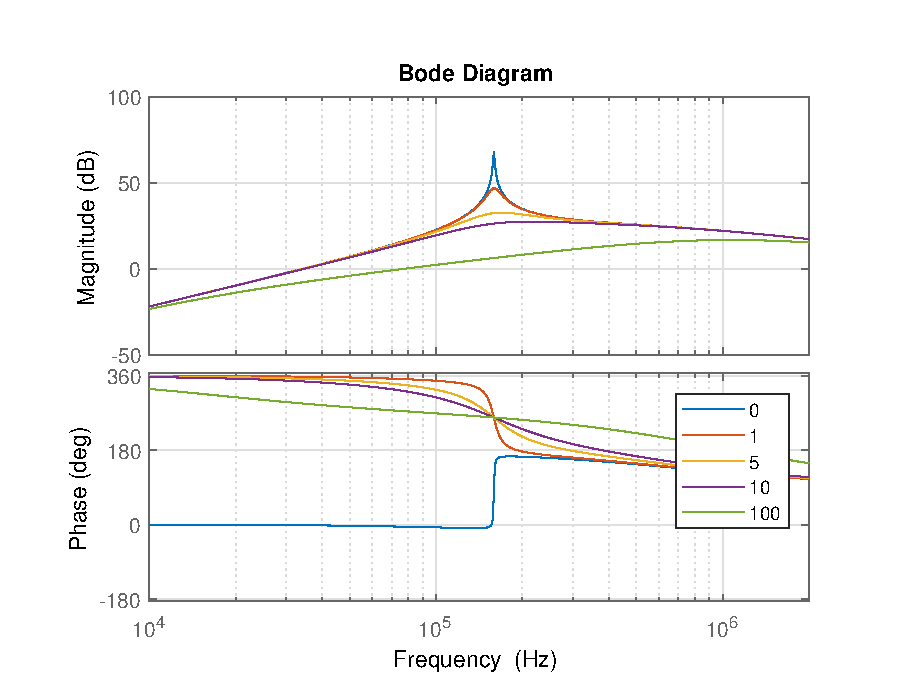
\includegraphics[width=\textwidth]{img/CoilRigBode_R1.eps}
    \caption{Bode plot of $H(j\omega)$ varying R1}
    \label{fig:bode_r1}
\end{figure}

Here we see that a lower resistance $R_1$ gives a sharper peak, and higher magnitude on the output.

\newpage
\Cref{fig:fbbode_r1} shows the bode plot of the transfer function for the current in the primary resonant circuit $H_{FB}(j\omega)$ with 5 different values for $R_1$, $0\Omega$, $1\Omega$, $5\Omega$, $10\Omega$, and $100\Omega$.
\begin{figure}[H]
    \centering
    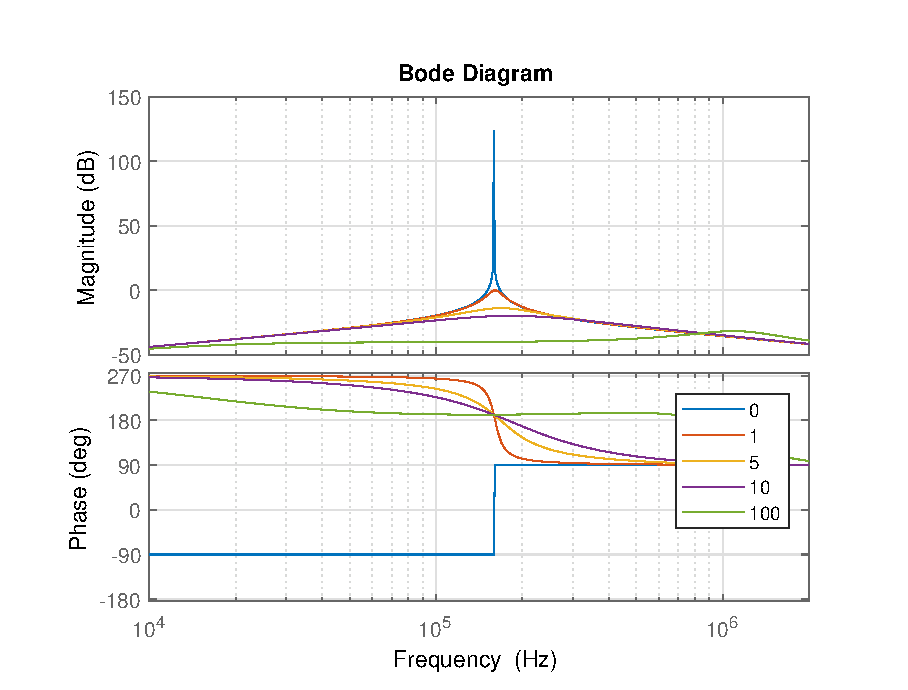
\includegraphics[width=\textwidth]{img/FeedBackBode_R1.eps}
    \caption{Bode plot of $H_{FB}(j\omega)$ varying R1}
    \label{fig:fbbode_r1}
\end{figure}

Here we see the same trend as in \cref{fig:bode_r1}, a lower resistance $R_1$ gives a sharper peak, and higher magnitude on the output. From this we can conclude that $R_1$ should be as low as possible. This is consistent with design recommendations in the hobby community, and the known formula for Q value for a single resonant circuit.

%%%%%%%%%%%%%%%%%%%%%%%%%%%%%%%%%%%%%%%%%%%%%%%%%%%%%%%%%%%%%%%%%%%%%%%%%%%%%%%%%%%%%%%%%%%%%%%%%%%%
\newpage
\Cref{fig:bode_r2} shows the bode plot of the transfer function for the resonant circuit $H(j\omega)$ with 5 different values for $R_2$, $0\Omega$, $1k\Omega$, $10k\Omega$, $100k\Omega$, and $1M\Omega$.

\begin{figure}[H]
    \centering
    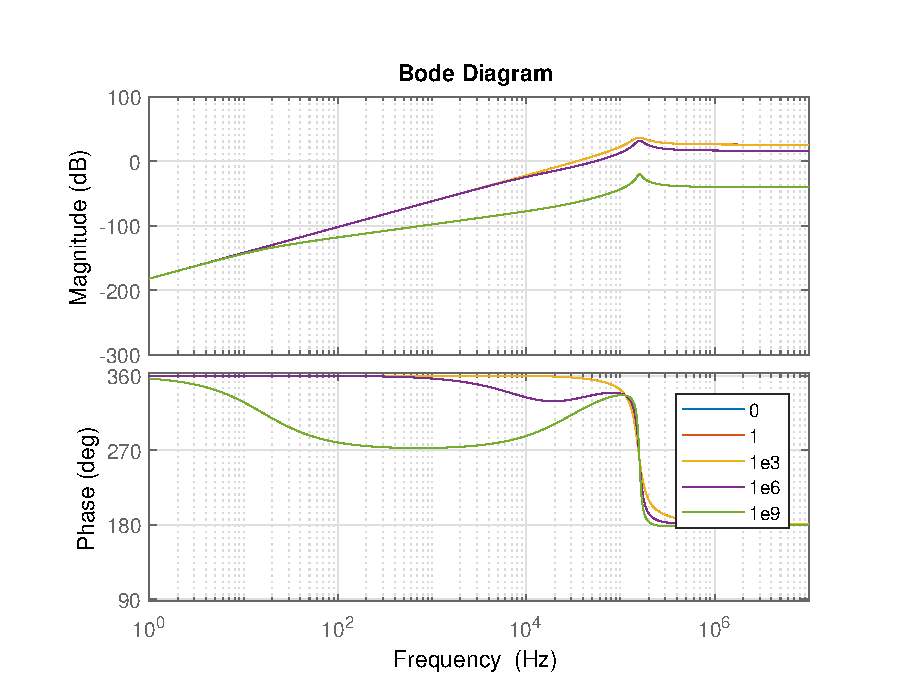
\includegraphics[width=\textwidth]{img/CoilRigBode_R2.eps}
    \caption{Bode plot of $H(j\omega)$ varying R2}
    \label{fig:bode_r2}
\end{figure}

Here we see that a lower resistance $R_2$ gives a higher magnitude on the output, but does not affect the sharpness of the peak.

\Cref{fig:fbbode_r2} shows the bode plot of the transfer function for the current in the primary resonant circuit $H_{FB}(j\omega)$ with 5 different values for $R_2$, $0\Omega$, $1\Omega$, $10\Omega$, $100\Omega$, and $1k\Omega$.
\begin{figure}[H]
    \centering
    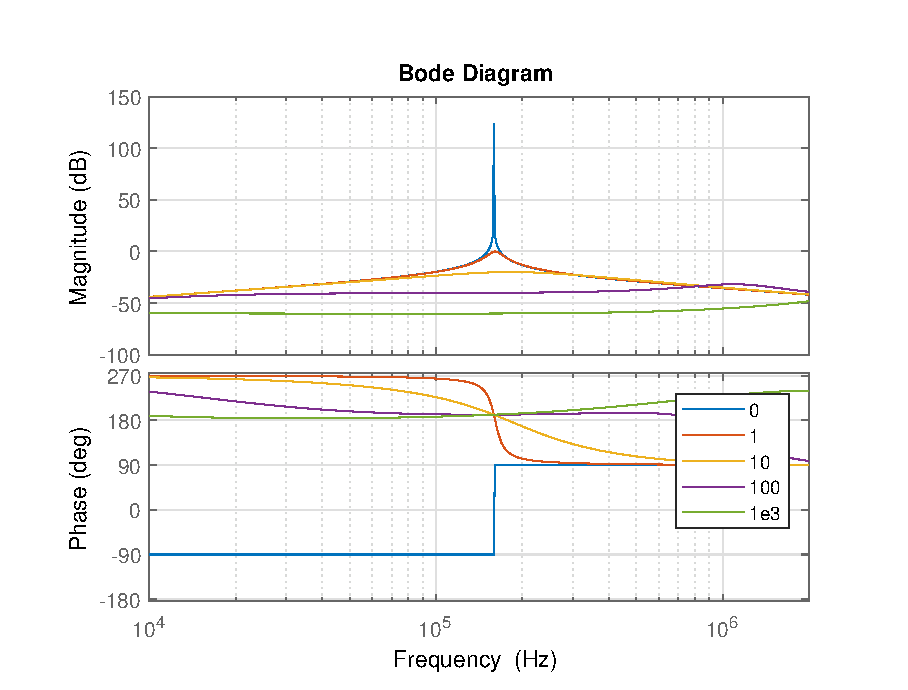
\includegraphics[width=\textwidth]{img/FeedBackBode_R2.eps}
    \caption{Bode plot of $H_{FB}(j\omega)$ varying R2}
    \label{fig:fbbode_r2}
\end{figure}

Here we see that a lower resistance $R_2$ gives a higher magnitude, and a sharper peak. From this we can conclude that $R_2$ should be as low as possible. This is consistent with design recommendations in the hobby community, and the known formula for Q value for a single resonant circuit.

%%%%%%%%%%%%%%%%%%%%%%%%%%%%%%%%%%%%%%%%%%%%%%%%%%%%%%%%%%%%%%%%%%%%%%%%%%%%%%%%%%%%%%%%%%%%%%%%%%%%
\newpage
\Cref{fig:bode_g1} shows the bode plot of the transfer function for the resonant circuit $H(j\omega)$ with 5 different values for $G_1$, $1e12{\Omega}^{-1}$, $1e3{\Omega}^{-1}$, $1e-6{\Omega}^{-1}$, $1e-12{\Omega}^{-1}$, and $0{\Omega}^{-1}$.

\begin{figure}[H]
    \centering
    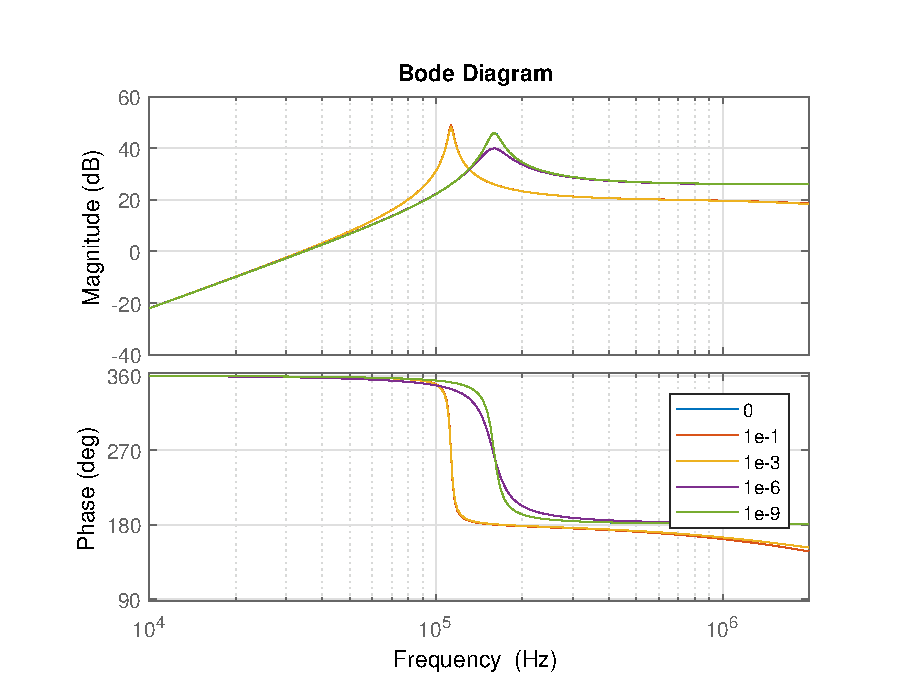
\includegraphics[width=\textwidth]{img/CoilRigBode_G1.eps}
    \caption{Bode plot of $H(j\omega)$ varying G1}
    \label{fig:bode_g1}
\end{figure}

Here we see that although we have a large range of values for $G_1$ the plots group in two, and there only seems to be a difference if $G_1$ is larger or smaller than 1. The top group of plots are a result of values larger than 1, and the lower group are a result of values smaller than 1. We cannot draw any significant conclusions from this.

\Cref{fig:fbbode_g1} shows the bode plot of the transfer function for the current in the primary resonant circuit $H_{FB}(j\omega)$ with 5 different values for $G_1$, $1e-3{\Omega}^{-1}$, $1e-4{\Omega}^{-1}$, $1e-4{\Omega}^{-1}$, $1e-5{\Omega}^{-1}$, and $0{\Omega}^{-1}$.
\begin{figure}[H]
    \centering
    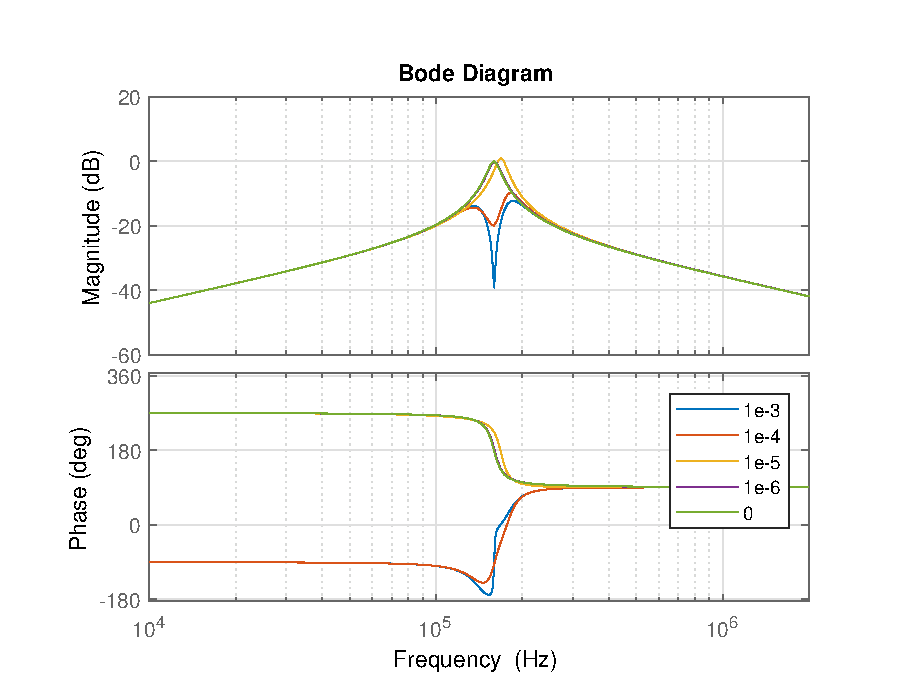
\includegraphics[width=\textwidth]{img/FeedBackBode_G1.eps}
    \caption{Bode plot of $H_{FB}(j\omega)$ varying G1}
    \label{fig:fbbode_g1}
\end{figure}

Here we see that when $G_1$ becomes larger than $~1e-5{\Omega}^{-1}$ we get a dip where the resonance peak was. This indicates we are unable to get any feedback signal. Thus $G_1$ should be smaller than $~1e-5{\Omega}^{-1}$, this is hard to control. This also implies that a streamer from the top load will affect the feedback signal, and with a too big streamer load the system with primary current feedback will be unable to function.

%%%%%%%%%%%%%%%%%%%%%%%%%%%%%%%%%%%%%%%%%%%%%%%%%%%%%%%%%%%%%%%%%%%%%%%%%%%%%%%%%%%%%%%%%%%%%%%%%%%%
\newpage
\Cref{fig:bode_k} shows the bode plot of the transfer function for the resonant circuit $H(j\omega)$ with 5 different values for $k$, 1.0, 0.5, 0.2, 0.1, and 0.001.

\begin{figure}[H]
    \centering
    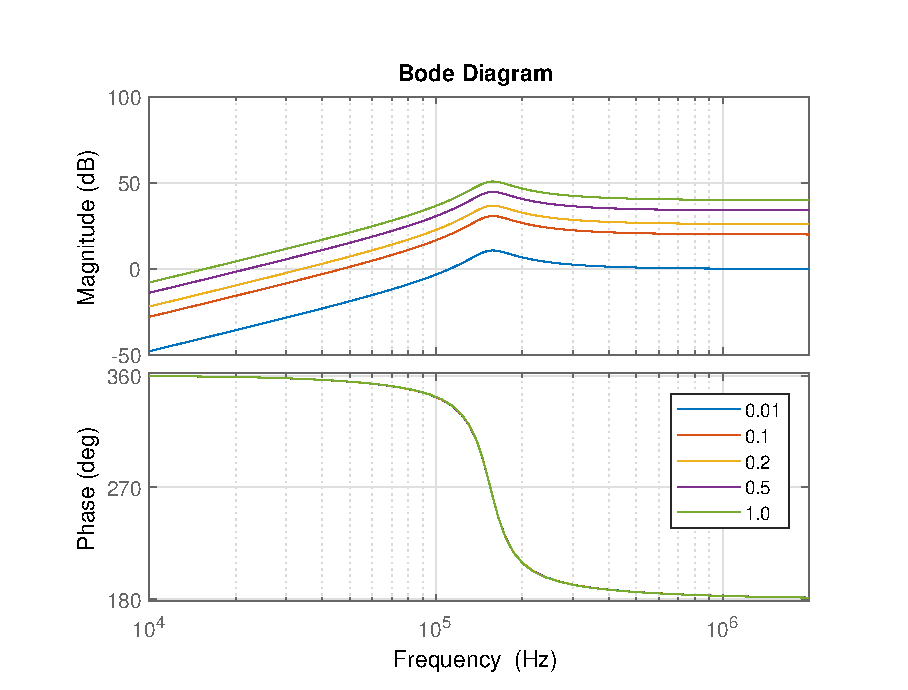
\includegraphics[width=\textwidth]{img/CoilRigBode_k.eps}
    \caption{Bode plot of $H(j\omega)$ varying k}
    \label{fig:bode_k}
\end{figure}

From this we see that the closer $k$ is to 1, the larger the magnitude, the sharpness and location of the peak does not seem to be affected.

\Cref{fig:fbbode_k} shows the bode plot of the transfer function for the current in the primary resonant circuit $H_{FB}(j\omega)$ with 5 different values for $k$, 1.0, 0.5, 0.2, 0.1, and 0.001.
\begin{figure}[H]
    \centering
    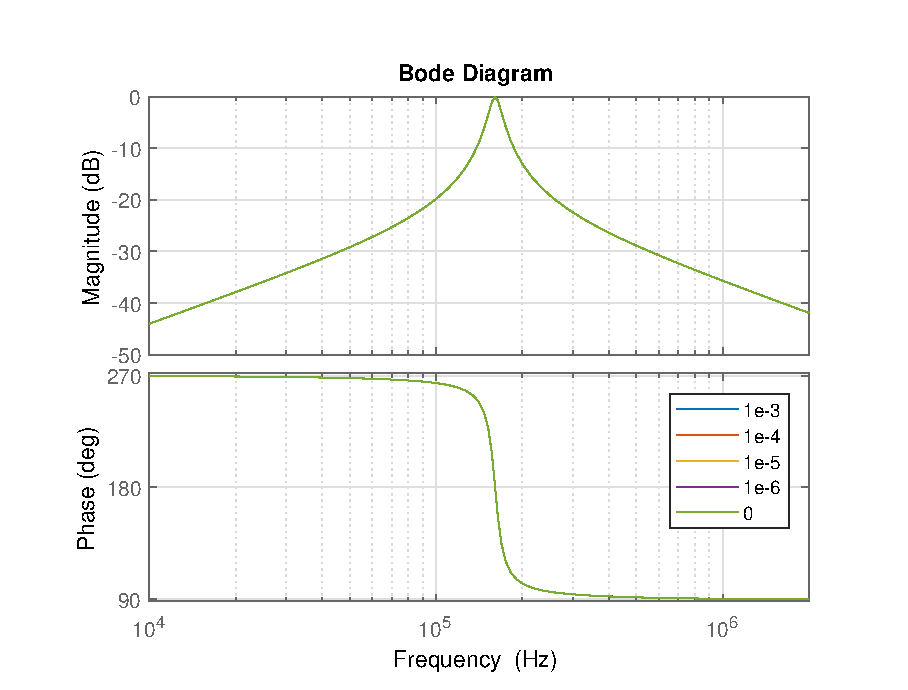
\includegraphics[width=\textwidth]{img/FeedBackBode_k.eps}
    \caption{Bode plot of $H_{FB}(j\omega)$ varying k}
    \label{fig:fbbode_k}
\end{figure}

Here we see no effect of varying $k$. From this it may seem that a $k$ of 1 is the best. But we know from the hobby community that a $k$ above to 0.2 causes significant risk of arcing between the primary and secondary coils \citep{scantesla} \citep{loneoceans} \citep{conner} \citep{easternvoltage} \citep{terrel} \citep{chunkyboy86}.

%%%%%%%%%%%%%%%%%%%%%%%%%%%%%%%%%%%%%%%%%%%%%%%%%%%%%%%%%%%%%%%%%%%%%%%%%%%%%%%%%%%%%%%%%%%%%%%%%%%%
\newpage
\Cref{fig:bode_c1} shows the bode plot of the transfer function for the resonant circuit $H(j\omega)$ with 5 different values for $C_1$, $0.1C_1$, $0.8C_1$, $1.0C_1$, $1.2C_1$, $10C_1$. Where $C_1 = 1 \cdot 10^{-7}$F.

\begin{figure}[H]
    \centering
    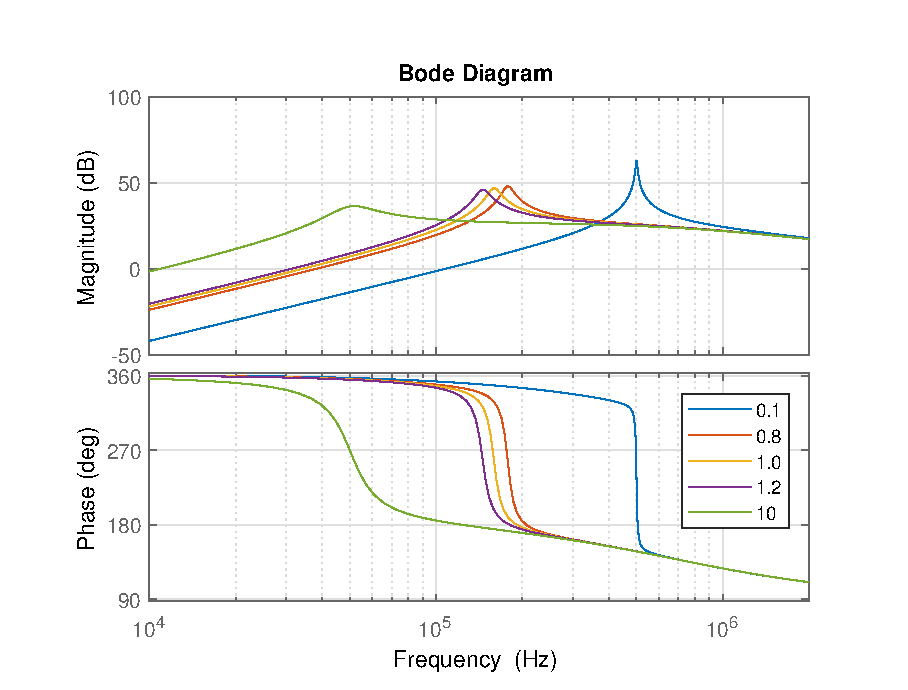
\includegraphics[width=\textwidth]{img/CoilRigBode_C1.eps}
    \caption{Bode plot of $H(j\omega)$ varying C1}
    \label{fig:bode_c1}
\end{figure}

From this we see that the resonance peak changes according to the change in $C_1$ as expected from the formula for resonance in a single resonance circuit. The magnitude seems to be a function of the resonance frequency, and it seems a larger magnitude may be obtained by reducing the value of $C_1$. This does not match with the hobby community recommendation of the two resonance frequencies needing to be the same.

\Cref{fig:fbbode_c1} shows the bode plot of the transfer function for the current in the primary resonant circuit $H_{FB}(j\omega)$ with 5 different values for $C_1$, $0.1C_1$, $0.8C_1$, $1.0C_1$, $1.2C_1$, $10C_1$. Where $C_1 = 1 \cdot 10^{-7}$F.
\begin{figure}[H]
    \centering
    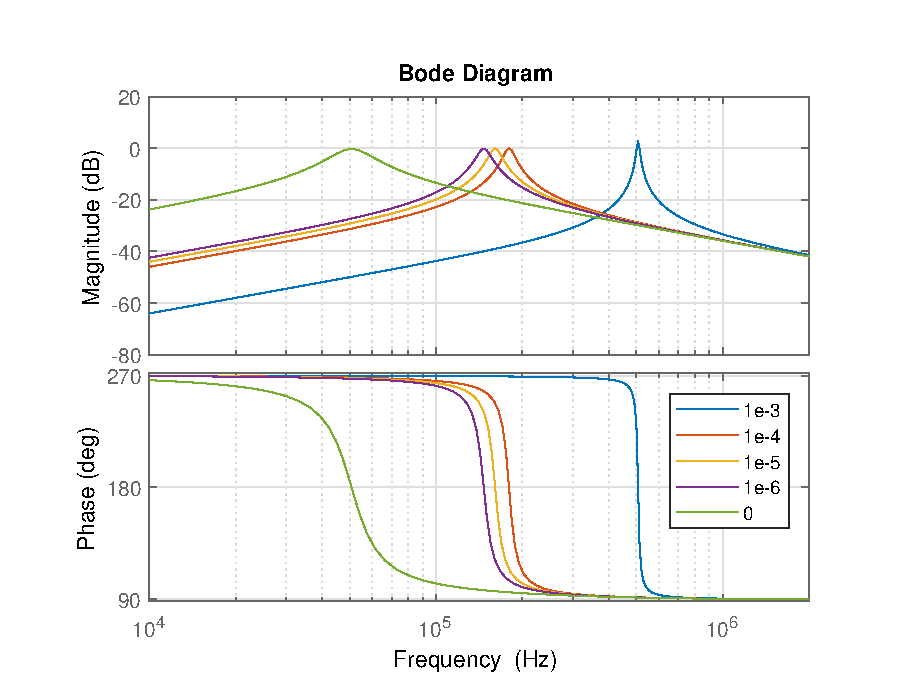
\includegraphics[width=\textwidth]{img/FeedBackBode_C1.eps}
    \caption{Bode plot of $H_{FB}(j\omega)$ varying C1}
    \label{fig:fbbode_c1}
\end{figure}

From this we see that the resonance peak changes according to the change in $C_1$ as expected from the formula for resonance in a single resonance circuit. The magnitude seems to stay the same.

%%%%%%%%%%%%%%%%%%%%%%%%%%%%%%%%%%%%%%%%%%%%%%%%%%%%%%%%%%%%%%%%%%%%%%%%%%%%%%%%%%%%%%%%%%%%%%%%%%%%
\newpage
\Cref{fig:bode_c2} shows the bode plot of the transfer function for the resonant circuit $H(j\omega)$ with 5 different values for $C_2$; $0.01C_2$, $0.1C_2$, $1.0C_2$, $10C_2$, $100C_2$. Where $C_2 = 1 \cdot 10^{-11}$F.

\begin{figure}[H]
    \centering
    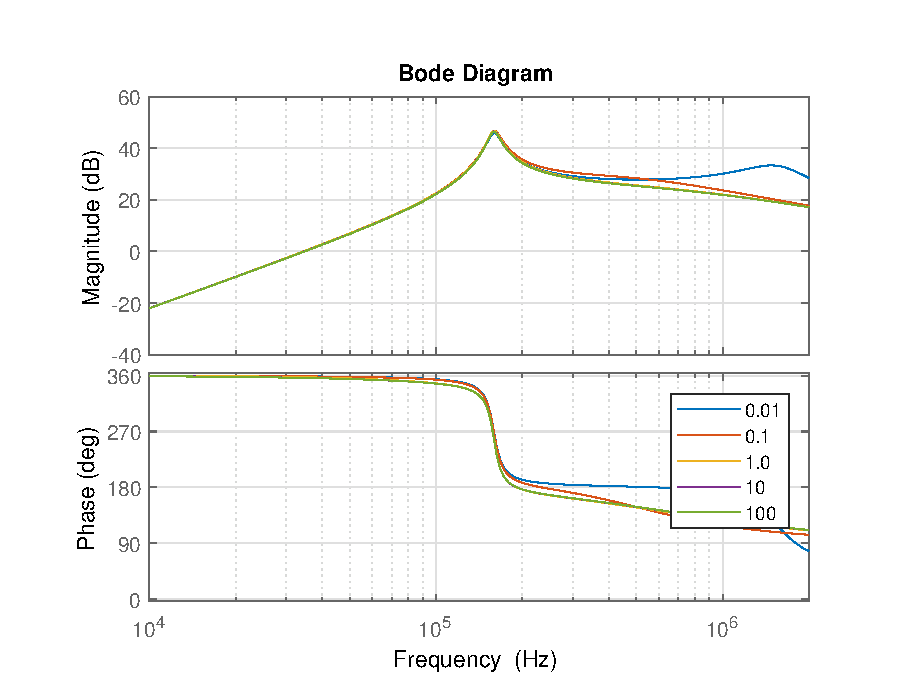
\includegraphics[width=\textwidth]{img/CoilRigBode_C2.eps}
    \caption{Bode plot of $H(j\omega)$ varying C2}
    \label{fig:bode_c2}
\end{figure}

Here we see very little change when varying $C_2$, we see a new peak forming when reducing $C_2$ to $0.001 C_2$.

\Cref{fig:fbbode_c2} shows the bode plot of the transfer function for the current in the primary resonant circuit $H_{FB}(j\omega)$ with 5 different values for $C_2$; $0.01C_2$, $0.1C_2$, $1.0C_2$, $10C_2$, $100C_2$. Where $C_2 = 1 \cdot 10^{-11}$F.
\begin{figure}[H]
    \centering
    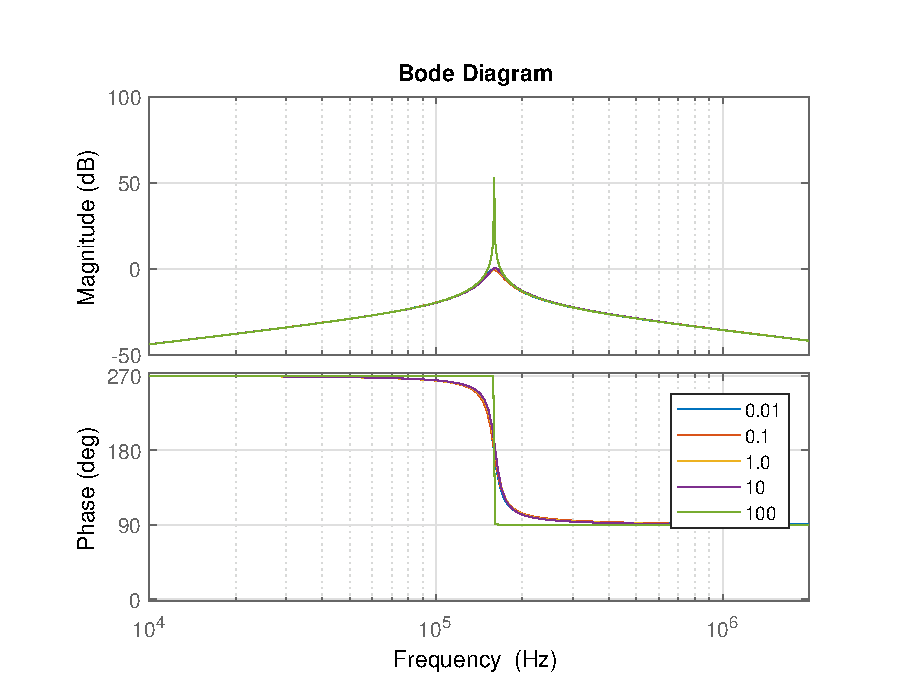
\includegraphics[width=\textwidth]{img/FeedBackBode_C2.eps}
    \caption{Bode plot of $H_{FB}(j\omega)$ varying C2}
    \label{fig:fbbode_c2}
\end{figure}

Here we see very little change when varying $C_2$. It may seem that varying $C_2$ has little effect. This does not match with the hobby community recommendation of the two resonance frequencies needing to be the same.

%%%%%%%%%%%%%%%%%%%%%%%%%%%%%%%%%%%%%%%%%%%%%%%%%%%%%%%%%%%%%%%%%%%%%%%%%%%%%%%%%%%%%%%%%%%%%%%%%%%%
\newpage
\Cref{fig:bode_l1} shows the bode plot of the transfer function for the resonant circuit $H(j\omega)$ with 5 different values for $L_1$; $0.1 L_1$, $0.8 L_1$, $1.0 L_1$, $1.2 L_1$, $10 L_1$, where $L_1 = 1 \cdot 10^{-5}$H.

\begin{figure}[H]
    \centering
    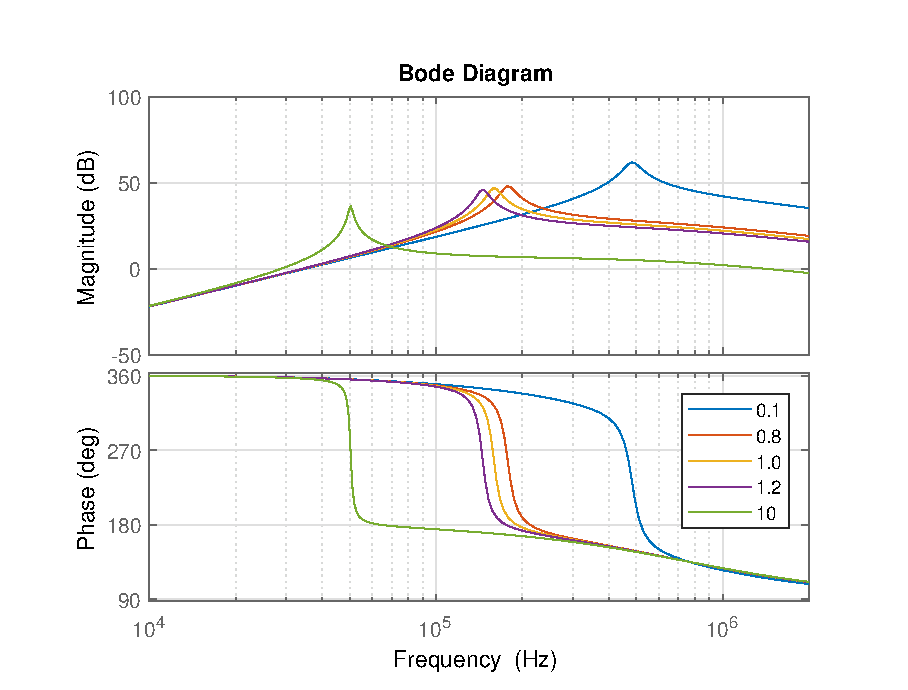
\includegraphics[width=\textwidth]{img/CoilRigBode_L1.eps}
    \caption{Bode plot of $H(j\omega)$ varying L1}
    \label{fig:bode_l1}
\end{figure}

From this we see that the resonance peak changes according to the change in $L_1$ as expected from the formula for resonance in a single resonance circuit. The magnitude seems to be a function of the resonance frequency, and it seems a larger magnitude may be obtained by reducing the value of $L_1$. This does not match with the hobby community recommendation of the two resonance frequencies needing to be the same.

\Cref{fig:fbbode_l1} shows the bode plot of the transfer function for the current in the primary resonant circuit $H_{FB}(j\omega)$ with 5 different values for $L_1$; $0.1 L_1$, $0.8 L_1$, $1.0 L_1$, $1.2 L_1$, $10 L_1$, where $L_1 = 1 \cdot 10^{-5}$H.
\begin{figure}[H]
    \centering
    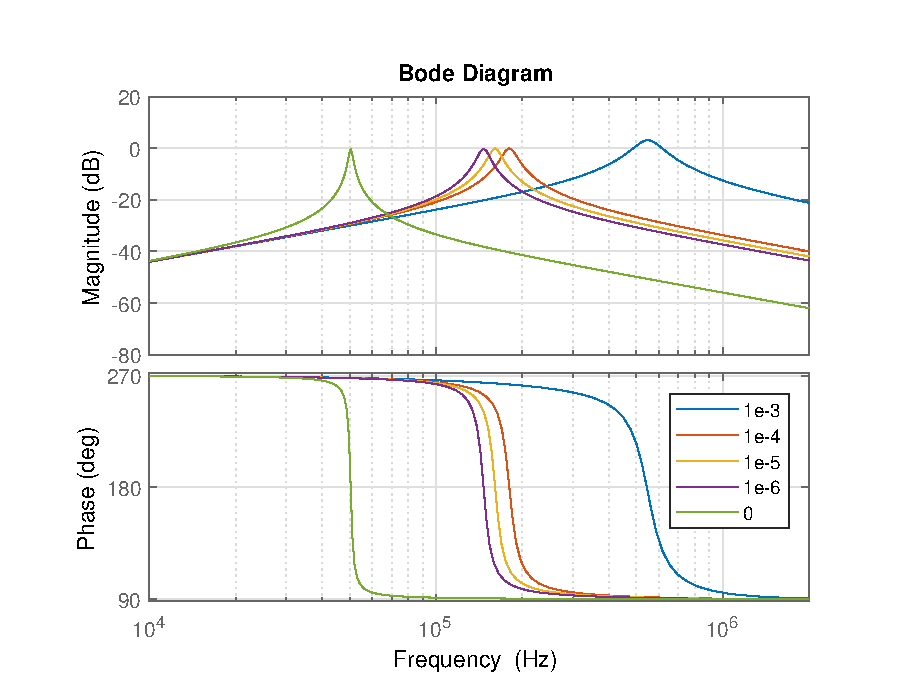
\includegraphics[width=\textwidth]{img/FeedBackBode_L1.eps}
    \caption{Bode plot of $H_{FB}(j\omega)$ varying L1}
    \label{fig:fbbode_l1}
\end{figure}

From this we see that the resonance peak changes according to the change in $L_1$ as expected from the formula for resonance in a single resonance circuit. The magnitude seems to stay the same.

%%%%%%%%%%%%%%%%%%%%%%%%%%%%%%%%%%%%%%%%%%%%%%%%%%%%%%%%%%%%%%%%%%%%%%%%%%%%%%%%%%%%%%%%%%%%%%%%%%%%
\newpage
\Cref{fig:bode_l2} shows the bode plot of the transfer function for the resonant circuit $H(j\omega)$ with 5 different values for $L_2$; $0.01 L_2$, $0.8 L_2$, $1.0 L_2$, $1.2 L_2$, $100 L_2$, where $L_2 = 1 \cdot 10^{-1}$H.

\begin{figure}[H]
    \centering
    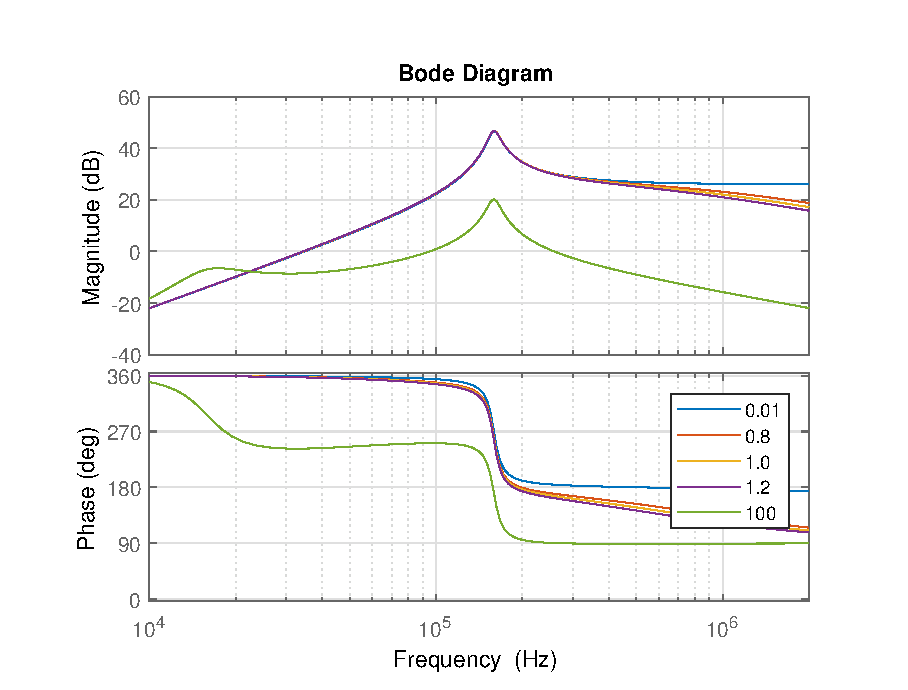
\includegraphics[width=\textwidth]{img/CoilRigBode_L2.eps}
    \caption{Bode plot of $H(j\omega)$ varying L2}
    \label{fig:bode_l2}
\end{figure}

Here we see little in resonance peak location or magnitude, apart from $100 L_2$ where the magnitude is drastically reduced.

\Cref{fig:fbbode_l2} shows the bode plot of the transfer function for the current in the primary resonant circuit $H_{FB}(j\omega)$ with 5 different values for $L_2$; $0.01 L_2$, $0.8 L_2$, $1.0 L_2$, $1.2 L_2$, $100 L_2$, where $L_2 = 1 \cdot 10^{-1}$H.
\begin{figure}[H]
    \centering
    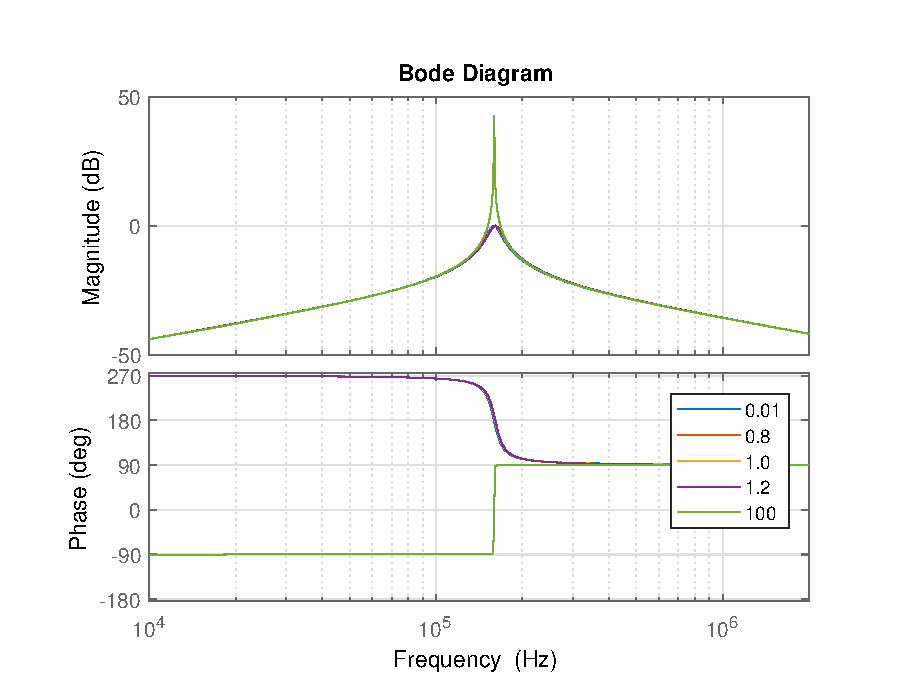
\includegraphics[width=\textwidth]{img/FeedBackBode_L2.eps}
    \caption{Bode plot of $H_{FB}(j\omega)$ varying L2}
    \label{fig:fbbode_l2}
\end{figure}
Here we see little in resonance peak location or magnitude, apart from $100 L_2$ where the magnitude is drastically increased. It may seem that varying $L_2$ has little effect. This does not match with the hobby community recommendation of the two resonance frequencies needing to be the same.

%Målebeskrivelse
\chapter{Methodology}

\section{Acoustic measurements}

The acoustic measurements of the tesla coil were performed in the high voltage laboratory at the department of electrical power engineering at ntnu. This was the only location fitting after health and safety considerations were made. This room is not designed for acoustic measurements, and has significant ambient noise and reflections.

The coil rig were placed in the room with a grounding electrode consisting an orb and spike with identical design as the topload placed a distance of ~40cm away. The driver was placed 3 meters away connected with a 3m long cable. The signal generator, pulse shaper, and recording equipment was placed adjacent to the driver.

The recording was performed by the department of acoustics at ntnu.

Since the room was not meant for acoustic measurements the impulse response of the room was measured. This measurement was also performed by the department of acoustics at ntnu. This was done by placing a speaker approximately in the center of the room, and a microphone were the microphone was to be placed during recordings. Then a sweep was played on the speaker, and recorded.

The recordings of single tones was performed by setting the signal generator to the wanted input frequency and then the output sound was recorded.

The recordings of musical audio files was performed by playing the file from a computer and then recording the output sound.

The sweep was recorded by playing a sweep from a different computer, and then recording, When playing the sweep we discovered that the computer playing back the sweep (and recording) was affected by the electromagnetic field generated by the tesla coil, and the playback was thus choppy. It was later discovered that all recordings done were choppy.

%Department of acoustics

%Impulse response of room measured first

%Recording is lagging, affected by electromagnetic field

%Recording of different (single) tones

%Recording of musical audio files

%Recording of sweep
%Måleresultater
%\chapter{Results}
%What are the measurement/model results

\chapter{Measurements}
To confirm that the signals X1-X9 have the alleged behaviour measurements have been done on a physically implemented DRSSTC, with the component values shown in the schematics in this thesis. The DRSSTC the measurements are done on is the one constructed by Omega Verksted \citep{prosjektoppgave} \citep{githubtesla}.


\section{Voltage measurements}
The voltage measurements of the tesla coil were performed in the high voltage laboratory at the department of electrical power engineering at NTNU.

\Cref{fig:m_x1-x2} shows the signal X1 into the pulse shaper and the resulting signal X2 on the output of the pulse shaper. The interrupter and power amplifier is not connected.

\begin{figure}[H]
    \centering
    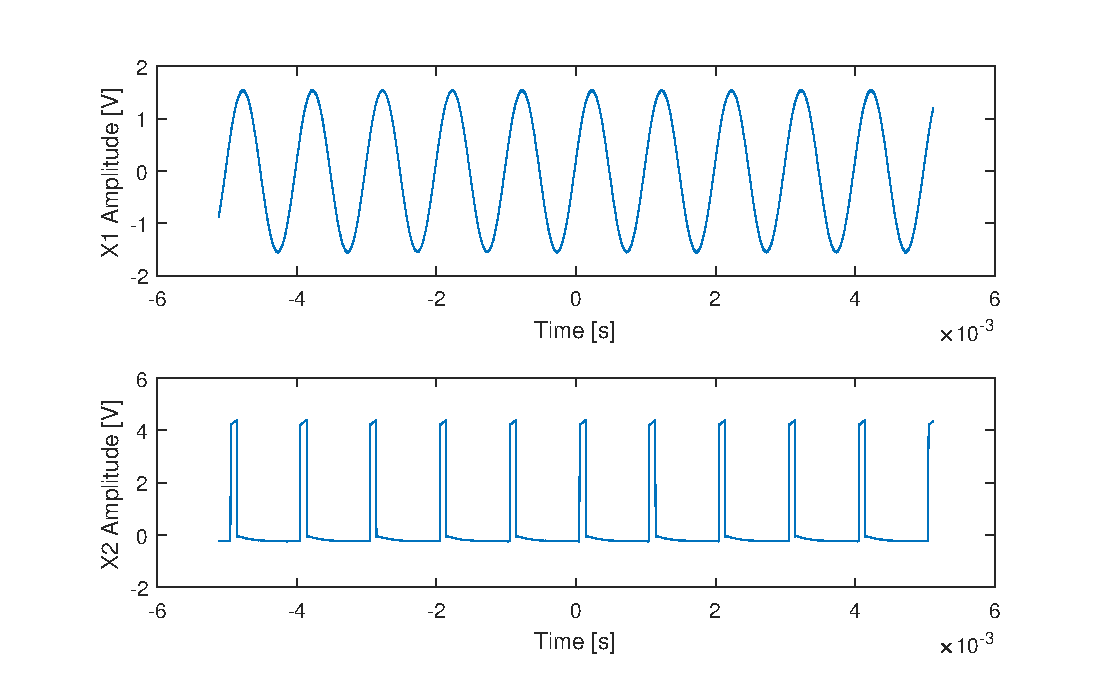
\includegraphics[trim={1cm 0cm 1cm 0cm},clip,width=\textwidth]{img/X1-X2.eps}
    \caption{X1 X2}
    \label{fig:m_x1-x2}
\end{figure}

Here we see that the sinusoidal signal X1 with zero DC component is transformed into a two level signal X2 between 0V and 5V. We also see that it has a constant duty cycle.

\Cref{fig:m_x1-x2-x4-x8} shows the same signals X1 and X2 as in \cref{fig:m_x1-x2} but also shows the output of the interrupter X4 as well as the feedback signal X8. Note that X2 is measured after the optical channel.

\begin{figure}[H]
    \centering
    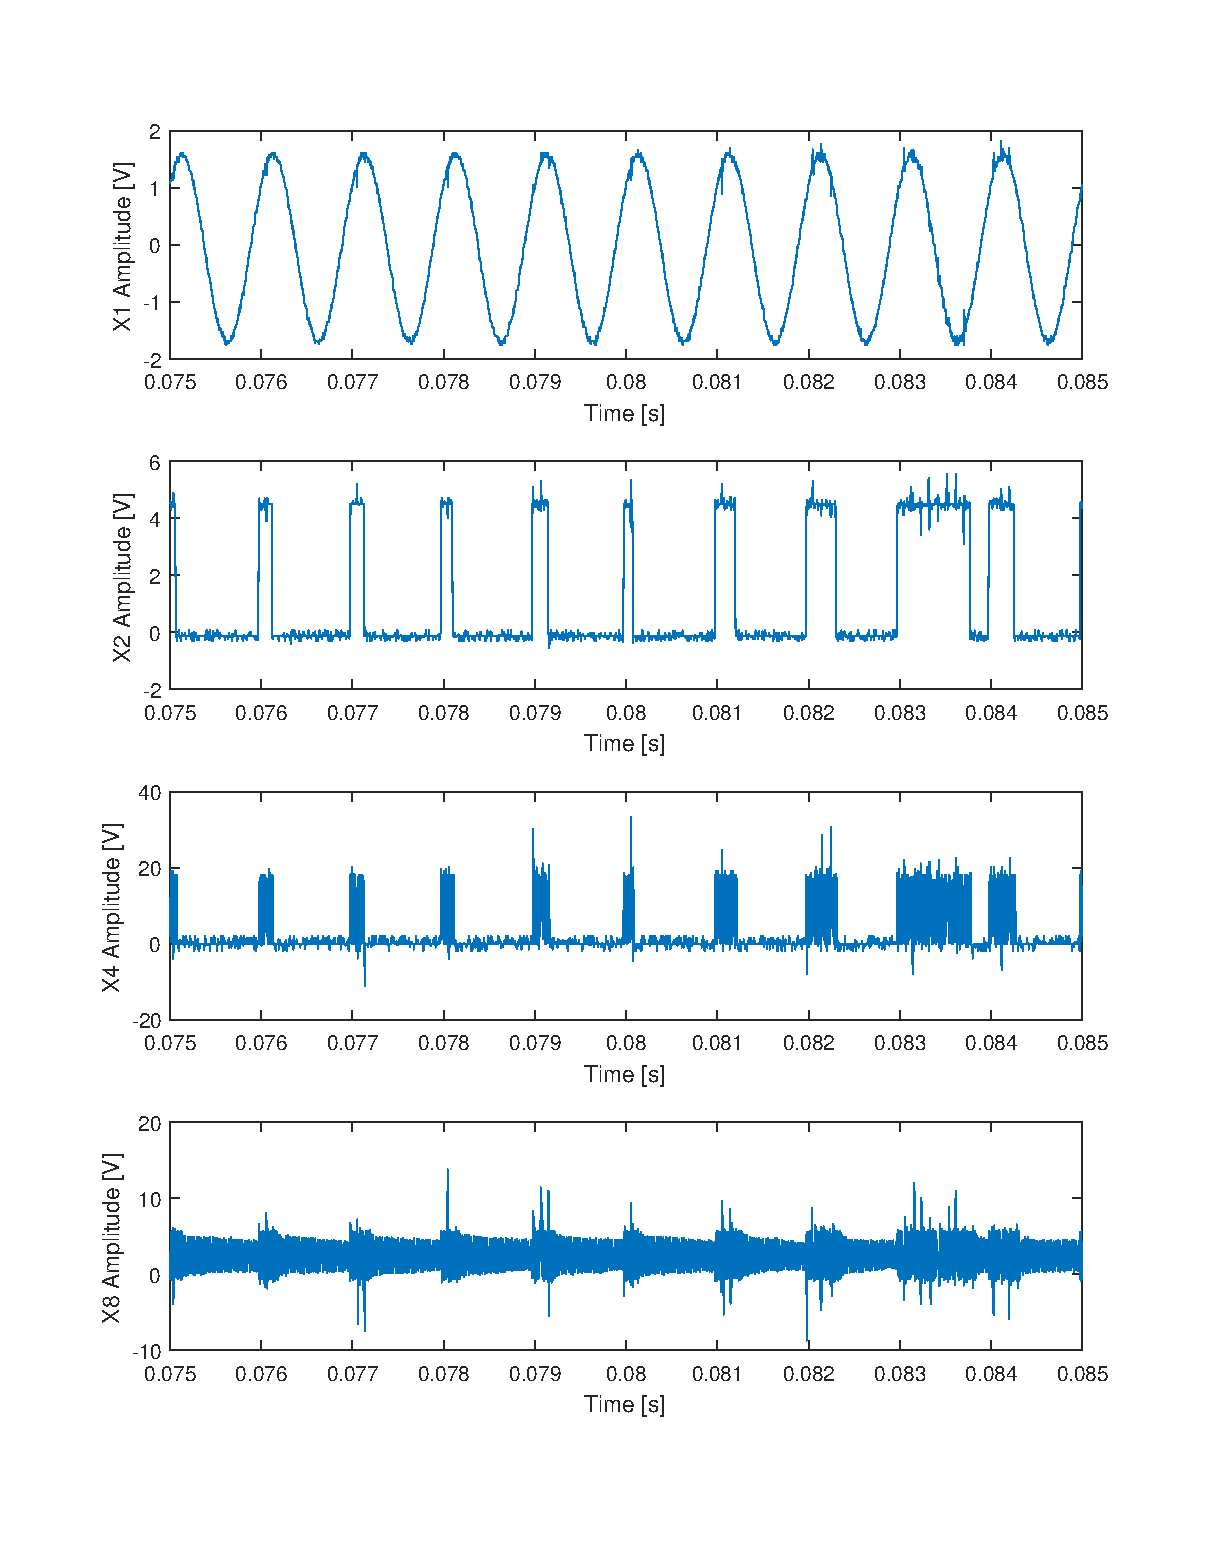
\includegraphics[trim={1cm 0cm 1cm 0cm},clip,width=\textwidth]{img/X1-X2-X4-X8.eps}
    \caption{X1 X2 X4 X8}
    \label{fig:m_x1-x2-x4-x8}
\end{figure}

First it is worth noting that we have more noise in \cref{fig:m_x1-x2-x4-x8} than in \cref{fig:m_x1-x2} because the interrupter, power amplifier, and resonant circuit are connected and turned on. We see that this electromagnetic noise affects how well X2 is generated, and the duty cycle is no longer constant. This is a source of noise on the output acoustic signal. The envelope of X4 follows X2 as expected. The envelope of X8 follows X2 as well as it having a ring down.

\Cref{fig:m_x6} shows the voltage on the output of the power amplifier $U_{X6}$.

\begin{figure}[H]
    \centering
    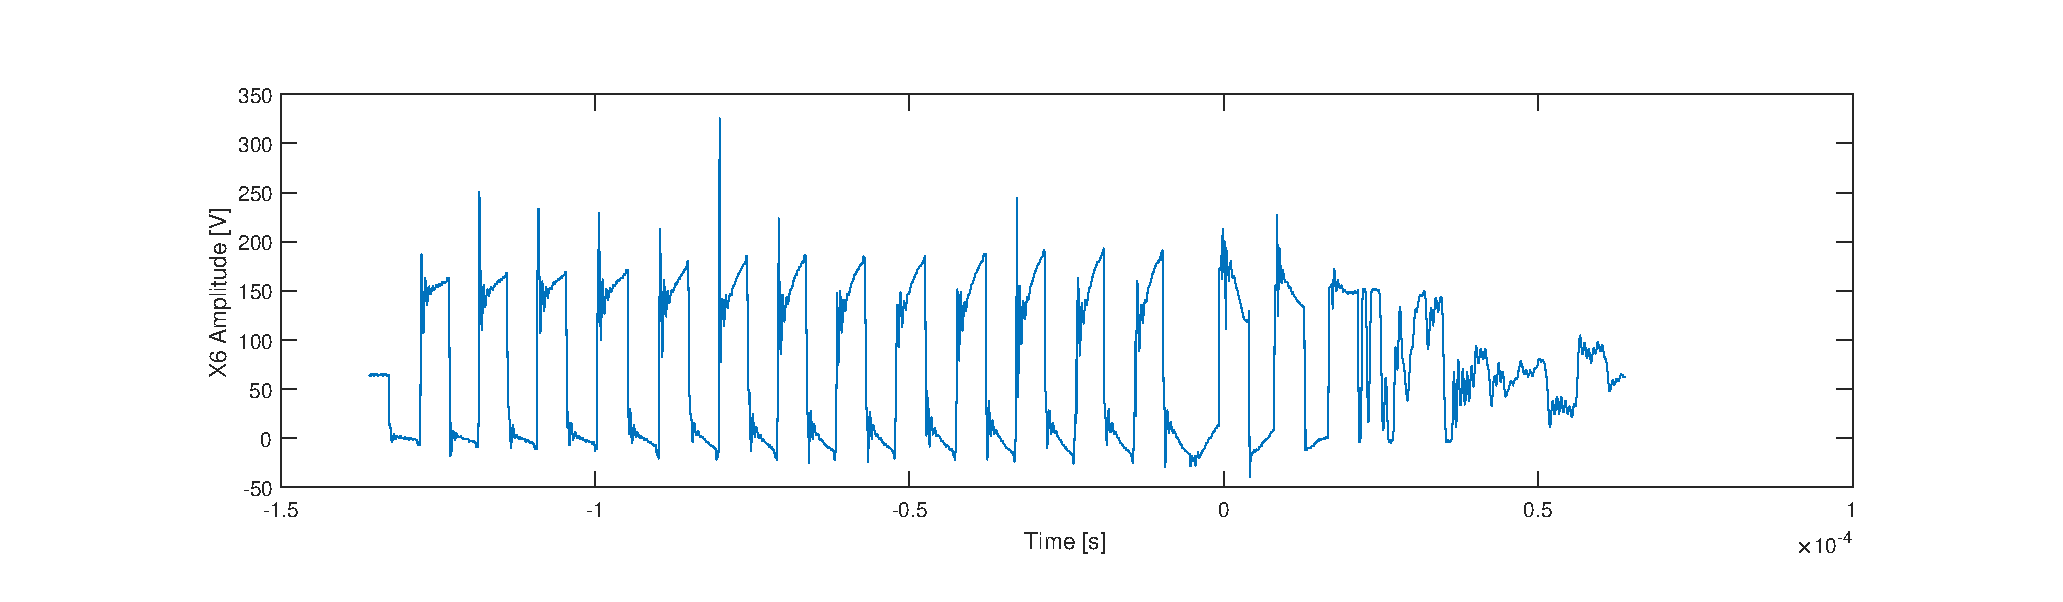
\includegraphics[trim={3.2cm 0cm 3.2cm 0cm},clip,width=\textwidth]{img/X6singlepulse.eps}
    \caption{X6}
    \label{fig:m_x6}
\end{figure}

Here we see a positive square wave with 50\% duty cycle and amplitude from 0V to 160V, and a duration of 13 cycles before being turned off. After this wave train we see the ring down of the voltage on the resonant circuit.

\newpage
\section{Acoustic measurements}

The acoustic measurements of the tesla coil were performed in the high voltage laboratory at the department of electrical power engineering at NTNU. This was the only location fitting after health and safety considerations were made. This room is not designed for acoustic measurements, and has significant ambient noise and reflections.

The coil rig were placed in the room with a grounding electrode consisting an orb and spike with identical design as the topload placed a distance of ~40cm away. The driver was placed 3 meters away connected with a 3m long cable. The signal generator, pulse shaper, and recording equipment was placed adjacent to the driver.

The recording was performed by the department of acoustics at ntnu.

Since the room was not meant for acoustic measurements the impulse response of the room was measured. This measurement was also performed by the department of acoustics at ntnu. This was done by placing a speaker approximately in the center of the room, and a microphone were the microphone was to be placed during recordings. Then a sweep was played on the speaker, and recorded.

The recordings of single tones was performed by setting the signal generator to the wanted input frequency and then the output sound was recorded.

The recordings of musical audio files was performed by playing the file from a computer and then recording the output sound.

The sweep was recorded by playing a sweep from a different computer, and then recording, When playing the sweep we discovered that the computer playing back the sweep (and recording) was affected by the electromagnetic field generated by the tesla coil, and the playback was thus choppy. It was later discovered that all recordings done were choppy.

The acoustic measurements done but not discussed here is attached in \cref{sec:appdx:akustisk}

%Department of acoustics

%Impulse response of room measured first

%Recording is lagging, affected by electromagnetic field

%Recording of different (single) tones

%Recording of musical audio files

%Recording of sweep

\Cref{fig:period_1k} shows a periodogram of the recorded audio signal with a 1kHz input on X2. The amplitude is the energy of the signal and the x-axis shows the frequency.
\begin{figure}[H]
    \centering
    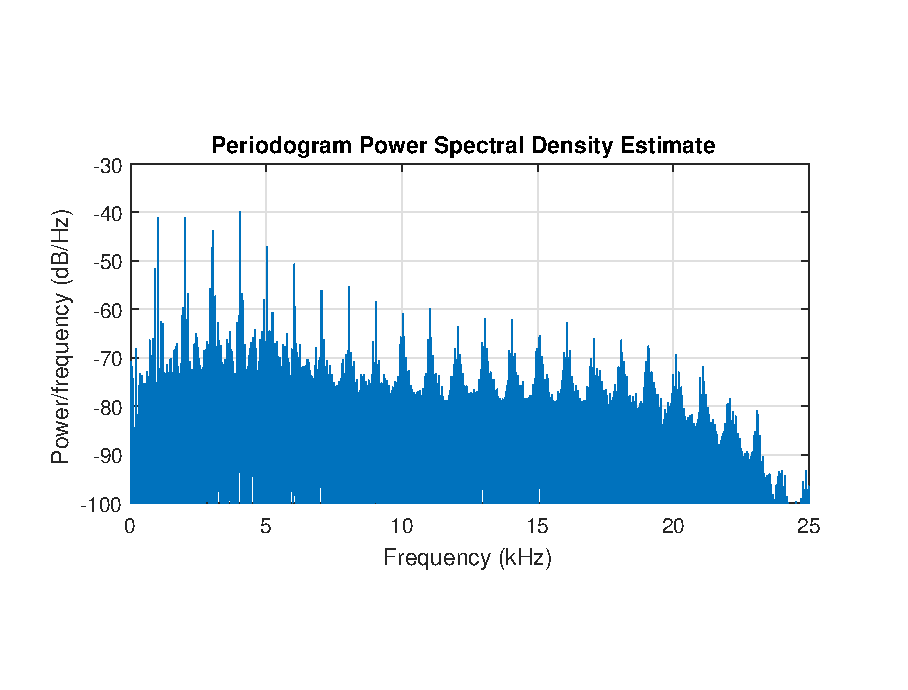
\includegraphics[trim={0cm 1.6cm 0cm 2cm},clip,width=\textwidth]{img/Periodogram_1khz-09.eps}
    \caption{Periodogram of 1kHz recorded tone}
    \label{fig:period_1k}
\end{figure}

Here we see the base frequency 1kHz and harmonics spaced 1kHz apart all the way through the range of human hearing. We see that the lowest three harmonics together with the base frequency are dominant, then the energy of the harmonics start to decrease. This implies the waveform rises sharply and has a short duration, which is consistent with a series of electrical discharges. The amplitudes of the harmonics are shown in \cref{tab:1k_amps}.

\Cref{fig:recorded_1k} shows the waveform of the recorded audio signal with a 1kHz input on X2.

\begin{figure}[H]
    \centering
    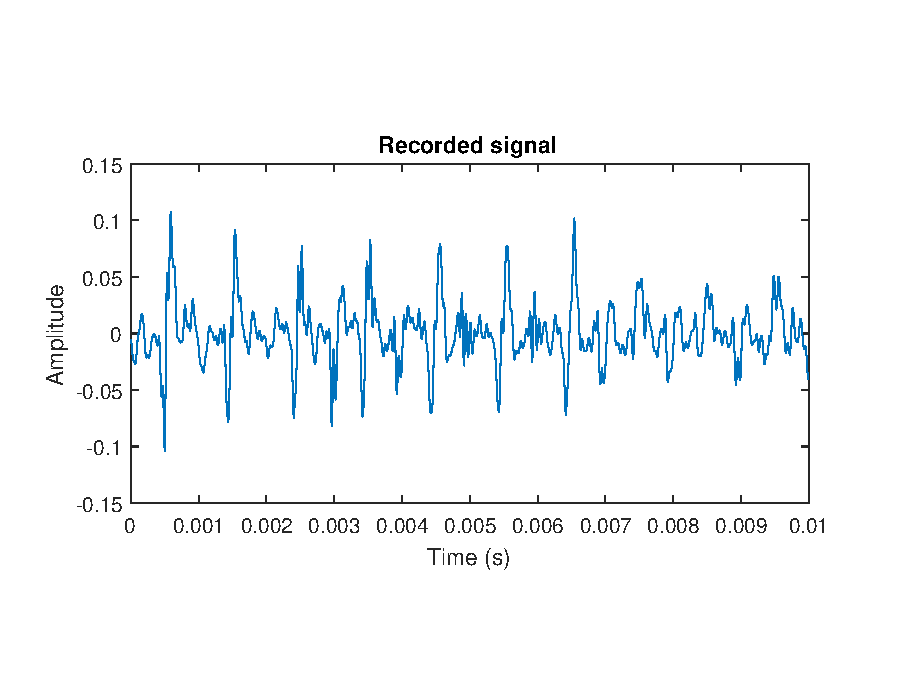
\includegraphics[trim={0cm 1.6cm 0cm 2cm},clip,width=\textwidth]{img/Recorded_1khz-09.eps}
    \caption{Time domain plot of 1kHz recorded tone}
    \label{fig:recorded_1k}
\end{figure}

Here we see a dominant series of pulses with frequency 1kHz, we also see that it has several higher harmonics. Which is consistent with \cref{fig:period_1k}. The signal also appears to be noisy.

%\begin{table}[]
%    \centering
%    \begin{tabular}{c|c|c|c|c|c|c|c|c|c|c|c|c|c|c|c|c|c|c|c|c|c|c}
%        Frequency (Hz)      & 1k  & 2k  & 3k  & 4k  & 5k  & 6k  & 7k  & 8k  & 9k  & 10k & 11k & 12k & 13k & 14k & 15k & 16k & 17k & 18k & 19k & 20k & 21k & 22k \\
%        Amplitude (dB/Hz)   & -41 & -41 & -44 & -40 & -47 & -51 & -55 & -55 & -58 & -60 & -60 & -64 & -62 & -62 & -65 & -62 & -66 & -66 & -67 & -70 & -72 & -80 \\
%    \end{tabular}
%    \caption{Caption}
%    \label{tab:my_label}
%\end{table}

\begin{table}[h]
    \centering
    \begin{tabular}{c|c}
        Frequency (Hz) & Amplitude (dB/Hz) \\
        1k  & -41 \\
        2k  & -41 \\
        3k  & -44 \\
        4k  & -40 \\
        5k  & -47 \\
        6k  & -51 \\
        7k  & -55 \\
        8k  & -55 \\
        9k  & -58 \\
        10k & -60 \\
        11k & -60 \\
        12k & -64 \\
        13k & -62 \\
        14k & -62 \\
        15k & -65 \\
        16k & -62 \\
        17k & -66 \\
        18k & -66 \\
        19k & -67 \\
        20k & -70 \\
        21k & -72 \\
        22k & -80
    \end{tabular}
    \caption{Amplitudes of the harmonics}
    \label{tab:1k_amps}
\end{table}

\Cref{fig:rectones} shows the recorded signal compared to a signal generated in matlab with the amplitudes read from the periodogram of the recorded signal and shown in \cref{tab:1k_amps}.

\begin{figure}[H]
    \centering
    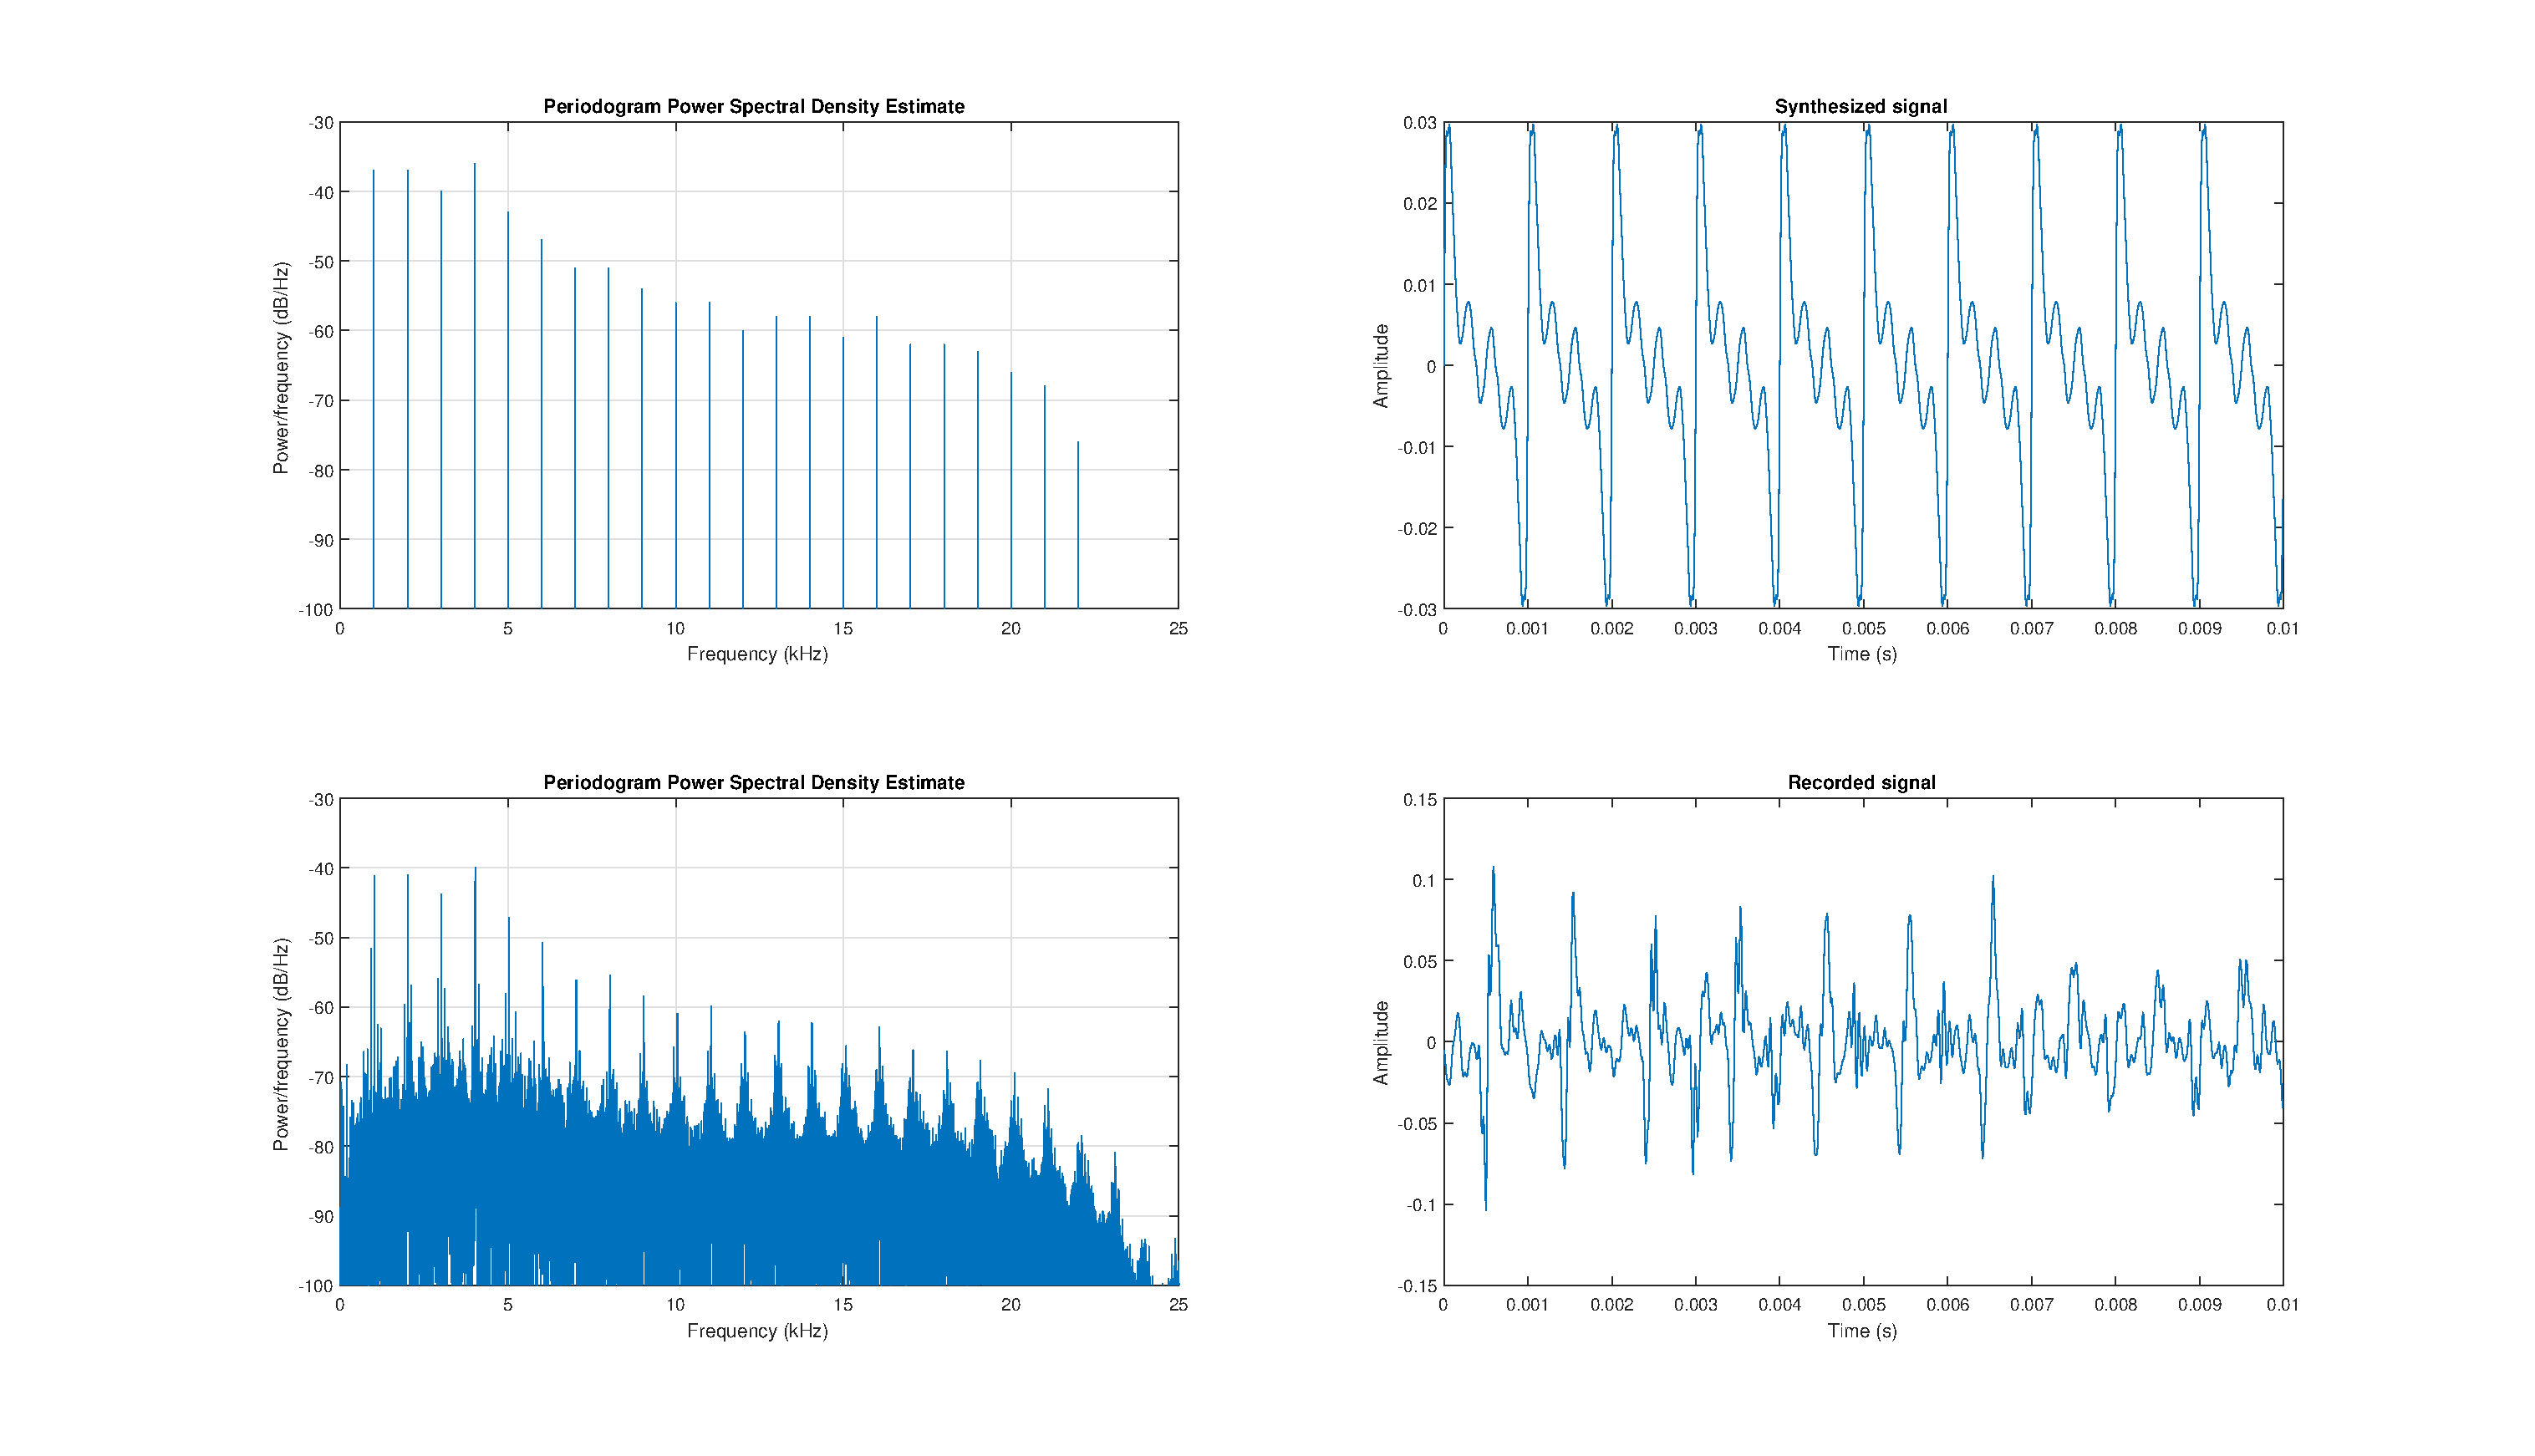
\includegraphics[trim={4cm 1.6cm 4cm 1.6cm},clip,width=\textwidth]{img/tones.eps}
    \caption{Comparison of recorded tone and synthesized tone}
    \label{fig:rectones}
\end{figure}

From this figure we see that the reconstructed signal matches well with the exception of the reconstructed signal not having any frequency components other than the harmonics.
%Diskusjon
%\chapter{Discussion}
How does the theory and practice fit together, is this acceptable? good enough? Unless done in results

%\begin{table}[]
%    \centering
%    \begin{tabular}{c|c|c}
%        Parameter   & Description           & Influence \\
%        1           & Input pulse length    & Spark length/Volume\\
%        2           & Reset network filter  & \\
%        3 ($f_c$)   & Limiter feedback filter limit frequency & \\
%        4           & Limiter current sense range  & \\
%        5           & Interrupter feedback Phase lead & \\
%    \end{tabular}
%    \caption{Parameters}
%    \label{tab:my_label}
%\end{table}
%\todo{Hvor skal dette?}

\section{Trigger pulse length}
The input pulse length is the time the triggering signal X2 is active (high) for each period. See \cref{triggering_signal} for a description of the triggering signal X2. The longer the triggering signal is active the more cycles are driven into the resonant circuit as explained in \cref{sec:interrupter}. When more cycles are driven into the resonant circuit the voltage on the output rises exponentially as seen in \cref{fig:linsim}, with higher voltage on the output a longer streamer (spark) can be produced as explained in \cref{sec:arc}. The relation between the input pulse length and the output streamer length is \todo{Find the relation}.
\todo{Relate to volume}

\section{Interrupter feedback voltage level}
\todo{Needs to be strong enough}

\section{Interrupter feedback phase lead}
The interrupter feedback phase lead is the phase lead introduced to the feedback voltage in the interrupter with relation to the current as described in \cref{sec:phaselead}. This gives a negative delay to compensate for the delay in the feedback loop from the current flowing in the primary circuit to the transistors driving the primary circuit. As we want to switch the transistors driving the primary circuit when the current flowing through them is as low as possible to give as low power dissipates in the transistors as possible and to be completely in phase with the step response which is ongoing in the resonant circuit to amplify the response as much as possible. 
\todo{Add plot proving in phase is better}
\todo{Calculate how much better}

\section{Reset network filter}
The reset network filter for the latch in the interrupter is explained in \cref{sec:reset_net}, this filter has no effect on spark length or tone quality as long as the feedback circuitry and synchronous shutdown works properly. But if the synchronous shutdown does not work properly. This filter should prevent or reduce noise from the interrupter not shutting down properly between each pulse on the input signal X2. This can also reduce the spark length if the spark is prevented from unintentionally continue longer than intended.
\todo{Doesen't affect spark length, tone quality?}

\section{Limiter feedback filter limit frequency}
The limiter feedback filter is explained in \cref{sec:limiter}, and its limit frequency decides how much noise is allowed through to the comparator and thus how often the spark is shut down early unintentionally due to noise. The spark being shut down unintentionally generates noise on the acoustic signal.
\todo{Affects noise on tone}
\todo{What kind of noise}

\section{Limiter feedback current sense range}
The limiter feedback is explained in \cref{sec:limiter} and the range of current that can be sensed and compared to the preset level is critical to the maximum spark length attainable and the range of spark lengths attainable. And thus affects the volume and dynamic range of the acoustic signal.
\todo{Affects volume range}

\section{Resistance in resonant circuit}
The resistance in the resonant circuit which is described in \cref{sec:resonant} affects the spark length. The resistance decides the Q value of the resonant circuit, and thus how much gain we get at resonance, and how distinct the resonance is.
\todo{Affects spark length}
\todo{Insert or reference plots}

\section{}

%Konklusjon
\chapter{Conclusion}
A implementation of a DRSSTC has been analyzed and described. The intended function of components have been presented and substantiated with mathematics. The component values or parameters that need to be adapted to the resonant frequency are; the delay in the latch reset network $t_r$ given by $R_3$ and $C_2$ in the interrupter, the phase lead time $t_d$ given by $L_1$ and $R_2$ in the interrupter, and the corner frequency of the noise filter $f_c$ given by $R_2$ and $C_3$ in the limiter. $t_r$ affects the acoustic signal if the synchronous shutdown in the interrupter does not function correctly. $t_d$ affects the heat generated in the power amplifier, and the amplitude on the output. $f_c$ can affect noise on the acoustic signal.

The component values or parameters that need to be adapted to the current flowing in the primary resonant circuit $I_1$ are; $|Z_L|$ given by $L_1$ and $R_2$ in the interrupter, $R_2$ in the limiter, and the number of turns $n$ on $L_3$ and $L_4$ in the primary resonant circuit. $|Z_L|$ affects. $R_2$ affects the range of amplitude attainable on the output. $n$ affects the selection of $|Z_L|$ and $R_2$.

In the resonant circuit we have proven that the ohmic resistances $R_1$ and $R_2$ in both the primary and secondary circuit should be as small as possible to give a high as possible amplitude on the output, the conductance of the streamer $G_1$ does not seem to affect the resonant frequency (detuning) or the amplitude on the output, but does affect the current in the primary resonant circuit. And will affect the feedback signals $X8$ and $X9$. The coupling coefficient $k$ only affects the amplitude on the output, as long as no arcing happens between the primary and secondary coils $L_1$ and $L_2$. According to the transfer functions $H(s)$ and $H_{FB}(s)$ varying $C_1$, $L_1$, $C_2$, or $L_2$ does not give the same results as expected from the common assumptions in the hobby community. Here no other conclusions can be drawn other that this may be a topic for further research.

The electrical measurements done on the physical implementation further substantiates the mode of operation of the driver. The acoustic measurements substantiates that a acoustic signal can be generated with the circuits presented here, and may be used for further research on the streamer and any alternative or related ways of generating an acoustic signal with a tesla coil. This report may also give an operator insight into what input signals $X1$ are suitable for this implementation of driver.


% Resonansfrekvens
%TK514 R3,C2 -> T
%TK514 L1, R2 -> t_d
%TK513 R2, C3 -> f_c

% Strøm
%TK514 L1, R2 -> |Z_L| feedbackspenning
%TK513 R2 -> feedbackspenning
% n1/n2 -> feedbackspenning


% Resonanskrets

%Videre arbeid
\section{Further work}
What should be done next.

%Inngående beskrivelse, analyse og dokumentasjon av en DRSSTC implementasjon.

%Introduksjon
%Beskrivelse av Tesla Coil / DRSSTC
%Tidligere arbeid
%Teori?
%Beskrivelse av arkitektur (Blokkoppbygning)
%Inngående beskrivelse av kretsene (inkludert designvalg)
%Inngående beskrivelse av signaler i kretsene
%Matematisk beskrivelse av så mye som mulig av kretsen(e)
%Målebeskrivelse
%Måleresultater
%Diskusjon
%Konklusjon
%Videre arbeid


\newpage
\bibliographystyle{plain}
\bibliography{ref}

%<<byman
%% Configuration of the header strings for the Appendices
%\renewcommand{\chaptermark}[1]{%
%  \markboth{\MakeUppercase{\appendixname\ \thechapter}}%
%  {\MakeUppercase{#1}}
%}
%\fancyhead[RE,LO]{}
%
%\appendix
%byman>>
%\include{FFF-APPDX} 



\end{document}
